\chapter{Revisão Bibliográfica}\label{referencial_teorico}
Neste capítulo, alguns conceitos fundamentais da pesquisa bibliográfica realizada serão explanados com o intuito de atingir os objetivos descritos na seção \ref{objetivos} e o entendimento da solução proposta neste trabalho. Serão abordados modelos de políticas, como as de controle de acesso e conflitos entre as mesmas. Temas como mineração de dados, aprendizagem de máquina, algoritmos de classificação, hiperparâmetros, técnicas de aprendizado de máquina como  as \textbf{RNA's} --\textit{Redes Neurais Artificiais} e as \textbf{SVM} --- \textit{Support Vector Machines} também serão descritos e suas definições teóricas serão discutidas. Ao final, serão descritos alguns trabalhos relacionados ao tema desta proposta de dissertação.

\section{Segurança de dados computacionais} \label{seguranca_informacao}
Para \citeonline[p. 264]{wang_conflicts_2010}, ``O controle de acesso e a segurança da informação estão intimamente relacionados'' e as informações e os dados disponíveis sofreram um aumento frenético nas últimas décadas, fato que gerou uma crescente preocupação com o correto tratamento destes dados e, principalmente com questões de \textit{segurança} relacionadas à \textit{proteção} destas informações que seguem, a cada ano sendo coletadas e acumuladas em ritmo vertiginoso \cite{alecrim2019, machado2014, lima_fraud_2012, fayyad1996, santos_segurancnos_2007}. 

Considerando, por exemplo, o ambiente corporativo, cf. \citeonline[p.1]{fontes_politicas}, a ``informação é um recurso essencial para toda organização, independentemente do seu porte e do seu segmento de atuação no mercado''. 

%Professora pediu para tirar - ficou melhor mesmo
%E o mesmo autor afirma que: 
%\begin{citacao}
%	É utilizando a informação que processos organizacionais funcionam, as pessoas podem %realizar suas atividades profissionais, a geração de conhecimento acontece e o %compartilhamento desse conhecimento é realizado. \cite[p.1]{fontes_politicas}
%\end{citacao}

Neste contexto, tanto a obtenção da informação é um processo importante quanto o são as formas de armazenamento e proteção, além, claro, o fato de que a análise e interpretação destes dados e informações tornam-se atividades essenciais para a manutenção de negócios e o próprio desenvolvimento da sociedade. \cite{Boscarioli2017} \cite{marciano_segurancda_nodate}.

A informação, como observa-se, é um recurso crítico para qualquer instituição exigindo, portanto, \textit{a adoção de políticas de segurança} adequadas que visem a sua proteção, salvaguarda e manutenção para que este ativo, tão significativo, mantenha seu valor, sua abrangência e importância dentro do cenário das organizações, governos e usuários comuns \cite{marciano_segurancda_nodate}. 

Isto porque assim como a quantidade de dados e informações cresce rapidamente, aumentam também, a cada ano, \textit{as ameaças} aos ativos de informação variando desde fraudes informáticas e sabotagens até vandalismo ou espionagem \cite{casaca_porque_2013}.

%PROFESSORA PEDIU PARA TIRAR - sofri tanto para fazer essa parte!
%Inicialmente, os sistemas de informação e aplicações eram basicamente militares e não ligados em redes, logo, os problemas de segurança se limitavam ao acesso físico aos equipamentos. Os problemas começaram a surgir com a necessidade do compartilhamento do processamento de informações e de recursos entre várias categorias de usuários, com diferentes níveis de acesso, o que levou ao desenvolvimento dos sistemas operacionais de tempo compartilhado (\textit{time-sharing}). O foco era, prioritariamente, garantir a segurança já que recursos como terminais de acesso, dispositivos de armazenamento, impressoras, programas e sistemas eram compartilhados e poderiam gerar problemas de segurança \cite{benz_universidade_nodate}. Assim, originou-se o problema clássico da segurança: ``omo fazer com que usuários autorizados possam ter acesso a determinadas informações, ao mesmo tempo em que os usuários não autorizados não possam acessá-las?'' \cite{nist_guttman_introduction_1995}

%Destarte, foi criado, em 1967, nos EUA, com a contribuição de órgãos governamentais como o Departamento de Defesa e a CIA um documento chamado ``\textit{Security Control for Computer System:Report of Defense Science Board}'' que marcou o início do processo oficial de criação de um conjunto \textit{de regras} para a segurança de computadores. Outras ações se seguiram ao redor do mundo. Em outra atitude, o Departamento de Defesa norte-americano formulou um plano que daria origem ao \textit{``The Orange Book''}, o documento que contém um conjunto abrangente de regras de segurança. Embora hoje seja considerado ultrapassado, teve grande importância e foi base para diversas iniciativas relativas à segurança da informação. \cite{goncalves_nbr_2013}

Nos primórdios da computação o mundo ainda não estava totalmente interconectado por redes de computadores, em especial, pela Internet que trouxe, além de inúmeros benefícios, diversos outros problemas de segurança da informação e representou um desafio novo à proteção dos dados das organizações, governos e usuários domésticos \cite{fontes_politicas}. 

Assim, para \citeonline{mukkamala_intrusion_2002}, observa-se que que a segurança da informação é uma questão de preocupação global séria. Pois, a complexidade, acessibilidade e capilaridade da Internet serviram para aumentar as ameças à segurança dos sistemas de informação.

\citeonline[p. 2]{fontes_politicas} afirma que, por exemplo, informações que antes estavam persistidas em relatórios e poderiam ser protegidas fisicamente em gavetas ou armários hoje podem ficar disponíveis na Internet e acessíveis no mundo todo. Mínimas falhas ou ações criminosas podem disponibilizar informações sigilosas ou privadas ou bloquear o acesso a informações críticas para a realização do objetivos da organização, como alguns ataques cibernéticos o fazem.

Portanto, para \citeonline{casaca_porque_2013}, estes ativos de informação \textit{devem ser protegidos} de ameaças através de estratégias e \textit{políticas de segurança  da  informação},  feitas com  base  em  modelos  e  métricas bem  conhecidas e previamente definidas, permitindo  às  organizações  melhorar  seu processo de segurança da informação.

%De acordo com \cite{benz_universidade_nodate}, as maiores ameaças à segurança da informação são, assim:
%\begin{citacao}
	%ataques deliberados a software; falhas técnicas ou erros de software; ato humano de falha ou erro; atos deliberados de espionagem ou transgressão; atos deliberados de sabotagem ou vandalismo; falhas técnicas ou erros de hardware; atos deliberados de furto/roubo; forças da natureza; comprometimento de propriedade intelectual; problemas de qualidade em provedores de serviços; obsolescência tecnológica; e atos deliberados de extorsão de informações.
%\end{citacao}
%
%Diante destas ameaças, sejam elas previsíveis ou extemporâneas, insere-se toda a área da segurança da informação que para cada tipo de ameaça tem diversas opções de soluções para diferentes tipos de organizações. \cite{doherty_information_2005} 
%
%Segundo \citeonline[p. 2]{fontes_politicas}:
%
%\begin{citacao}
%	O que diferencia o uso da informação entre as organizações é a necessidade de disponibilidade, a exigência de integridade e o rigor em relação ao sigilo que cada organização precisa para a sua informação.
%\end{quote}
%
%E continua, declarando que:
%\begin{quote}
%		O grau de disponibilidade, integridade e confidencialidade (sigilo) protegerá a informação para que a organização operacionalize os seus negócios e atenda aos seus objetivos. \cite[p. 2]{fontes_politicas}
%\end{quote}

Assim, cf. \citeonline{doherty_information_2005}, como as informações são um ativo corporativo crítico que se tornou cada vez mais vulnerável a ataques de vírus, hackers, criminosos e erros humanos, as organizações precisam priorizar a segurança de seus sistemas para garantir que seus ativos de informação mantenham sua precisão, confidencialidade e disponibilidade. 

Uma das muitas formas de prover essas características, confidencialidade, confiabilidade é usando políticas de controle de acesso que garantem, mediante o estabelecimento de diretrizes, especificações e normas, a proteção e disponibilidade das informações dos sistemas. \cite{bellettini_role_2001} \cite{ueda_tese_2012}.

%Na mesma linha, \citeonline[p. 4]{fontes_politicas}, afirma que ``as organizações precisam implantar um processo de segurança da informação, e este processo deve ser considerado um ativo da organização, como tantos outros''.

%Para \citeonline{doherty_information_2005}, um mecanismo cada vez mais importante para proteger as informações corporativas e, ao fazer isso, reduzir a ocorrência de violações de segurança, é a formulação e aplicação de uma \textit{política} formal de segurança da informação nas organizações. [grifo do autor]

%\section{Políticas em sistemas de segurança computacionais} \label{politicas_sistemas_seguranca}

%Para proteger os sistemas de informação dos níveis crescentes de ameaças cibernéticas, as organizações são praticamente obrigadas a instituir programas (e controles) de segurança. Neste contexto, as \textit{políticas de segurança da informação} são uma base imprescindível dos programas de segurança organizacional \cite{knapp_information_2009} \cite{simon_administrative_1997}.

%\citeonline[p. 402]{hone_information_2002} consideram que ``o mais importante desses controles [e programas de segurança] é a política de segurança da informação''. E \citeonline{whitman_information_2001}, afirmam que o desenvolvimento de uma política de segurança da informação é o primeiro passo para preparar uma organização contra ataques de fontes internas e externas.

%Para \citeonline{straub_effective_1990}, a política de segurança da informação trata da integridade, disponibilidade e confidencialidade dos dados eletrônicos mantidos e transmitidos entre os sistemas de informação e é a condição prévia para a implementação de outros obstáculos eficazes.

%Uma política é uma regra geral que foi estabelecida em uma organização para limitar a circunspecção dos subordinados a ela. \citeonline{simon_administrative_1997}. Pode também ser entendida como regras que governam as escolhas no comportamento de um sistema \cite{sloman_security_2002} \cite{moffett_policy_1994}.

%No domínio dos sistemas de informação, a política foi definida em um contexto de planejamento e controle para estabelecer limites de comportamento aceitável, conflitos de decisão e padrões \cite{davis_management_1984}. 

%As políticas são especialmente relevantes para a segurança dos sistemas de informação, pois fornecem as bases para um programa geral de segurança e criam uma plataforma para implementar práticas seguras em uma organização \cite{von_solms_policies_2004}. 

%Em todos os trabalhos citados nesta \autoref{politicas_sistemas_seguranca} seus autores referem-se às políticas de segurança de \textit{alto nível}, em âmbito \textit{regulatório} e \textit{completo} \cite{monteiro_adocao_2017}.

\section{Controle de acesso}\label{sec:controle_acesso}
Para \citeonline{knapp_information_2009}, o objetivo de uma política é fornecer orientação gerencial e suporte à segurança da informação de acordo com os requisitos de negócios, as leis e regulamentos relevantes em determinada organização ou instituição. A política de segurança em um sistema computacional garante, portanto, a proteção de suas informações. Dentre as diversas tecnologias utilizadas para assegurar essas propriedades, temos, por exemplo, o controle de acesso \cite{sarkis:artigo:2016}

Para  \citeonline{wang_conflicts_2010}, o controle de acesso é o mecanismo central para atingir os requisitos de segurança em  sistemas  de  informação. Dessa forma,  trata-se  de  uma  tecnologia indispensável para quem faz uso de qualquer tipo de sistema, podendo basear-se ou coexistir com outros serviços de segurança \cite{sandhu:1996}.

Nas palavras de \citeonline[p. 264]{wang_conflicts_2010}:
\begin{citacao}
Especificamente, o controle de acesso pode ser usado para obter confidencialidade, integridade e privacidade de dados, garantindo que cada acesso a um sistema de informação e seus recursos sejam controlados de acordo com um conjunto de políticas predefinidas	
\end{citacao}

\citeonline[p. 8]{kropiwiec_policy_nodate} afirma que ``para entender o que é e como funcionam os mecanismos de controle de acesso de um sistema [...], faz-se necessário classificar os elementos do sistema em três grupos.'' Que são, segundo este autor, o conjunto de \textit{sujeitos}, de \textit{objetos} e o de \textit{ações}.

De acordo com \citeonline[p. 8]{kropiwiec_policy_nodate}, o \textit{conjunto de sujeitos} ``englobam qualquer elemento que pode realizar ações sobre objetos, e é composto por usuários, processos e o próprio sistema''. Já o \textit{conjunto de objetos} ``englobam os elementos sobre os quais podem ser realizadas ações''. E, por sua vez, o \textit{conjunto de ações} ``compreende a lista de ações que podem ser realizadas sobre cada um dos objetos do sistema''. Como, por exemplo, ler, escrever, apagar, abrir conexão, enviar mensagem, encerrar conexão entre muitas outras ações relativas a cada sistema em particular.

Os mecanismos de controle de acesso, portanto, verificam todas as requisições de dados e recursos administrados pelos sistemas definindo, assim, as circunstâncias nas quais as requisições de acesso são permitidas ou negadas \cite{sandhu:1996}. 

Desta forma, tanto as informações quanto os ativos do sistema mantém um nível adequado de segurança, conservam o sigilo e estabelecem importantes providências quanto ao acesso a informações, recursos confidenciais ou protegidos \cite{wang_conflicts_2010}.

Com o controle de acesso o usuário fica limitado apenas a execução de operações e ações no sistema que lhe foram previamente concedidas. Ao requerer acesso ao conteúdo de informações ou permissão de uso de recursos estes só serão outorgados a quem possui o direito de acesso aos mesmos \cite{ferraiolo_proposed_2001}.

Os modelos de controle de acesso fornecem um conjunto de regras e mecanismos para o funcionamento seguro dos sistemas, sendo responsáveis pela definição de políticas específicas de controle de acesso. Para \citeonline{monteiro_adocao_2017}, as políticas são diretrizes de \textit{alto nível} que determinam como os acessos são controlados e decisões de acessos são estabelecidas \cite{di_vimercati_policies_2005} \cite{sarkis2017} \cite{lopes_adopcao_2012}.

Para \citeonline[p. 264]{wang_conflicts_2010},
\begin{citacao}
	Os modelos de controle de acesso fornecem representações formais dos sistemas de controle de acesso. As políticas de controle de acesso são requisitos de segurança que descrevem como o acesso é gerenciado, quais informações podem ser acessadas por quem e sob quais condições essas informações podem ser acessadas
\end{citacao}

E conclui, ``os modelos de controle de acesso fornecem maneiras de pensar sobre as políticas que eles mantém e comprovam as propriedades de segurança do sistema''. \cite[p. 264]{wang_conflicts_2010},

Embora não seja o escopo deste trabalho é importante salientar que existem vários modelos, na literatura, de controle de acesso. Entre os principais, pode-se citar, o controle de acesso discricionário (\textit{Discretionary Acces Control} - DAC); o controle de acesso mandatório (\textit{Mandatory Access Control} - MAC); o controle e acesso baseado em papéis (\textit{Role-Based Access Control} - RBAC) e o controle de acesso baseado em relacionamentos (\textit{Relationship-Based Access Control} - ReBAC). Há também os mais recentes, ABAC (Attribute-based Access Control) e o baseado em funções de atributo, RABAC (Role and Attribute-based Access Control).

O modelo de políticas adotado neste trabalho está fundamentado exatamente como o proposto por \citeonline{sarkis2017} e \cite{sarkis:artigo:2016}. Este modelo está, também, baseado nos propostos pelos autores \citeonline{cuppens_high_2007}, além do trabalho de \citeonline{elrakaiby_formal_2012}, bem como no artigo de \citeonline{kalam_organization_2003} por dois motivos:
\begin{itemize}
	\item Este modelo ser suficientemente genérico, conforme demonstrado no texto de \cite{sarkar_2017};
	\item Este específico modelo abarcar, de forma conveniente e coerente, características importantes dos padrões RBAC e ReBAC.
\end{itemize}

A respeito do ABAC e do RABAC indica-se o artigo de \citeonline{qi_di_li_formal_2018}. Sobre o DAC e o MAC, sugere-se os trabalhos de \citeonline{sandhu:1996} e \citeonline{di_vimercati_policies_2005}. Sobre RBAC, recomenda-se \citeonline{ferraiolo_proposed_2001} e \citeonline{sandhu:1996}. Sobre o ReBAC aconselha-se seguir o trabalho de \citeonline{bui_efficient_2019} e \citeonline{fong_relationship-based_2011}.

\subsection{Políticas de Controle de acesso}\label{controle_acesso}

Uma política de controle de acesso tem como objetivo definir ou limitar o comportamento atual ou futuro de \textit{sujeitos} e \textit{objetos} para garantir que as suas \textit{ações} estejam alinhadas com os objetivos da empresa de acordo com o escopo de acesso de cada sujeito ou grupo de sujeitos, com as permissões, proibições ou obrigações que estes tenham sobre os objetos e quais dados ou recursos lhe são concedidos \cite{dunlop_dynamic_2002}\cite{sarkis2017}.

As políticas de controle de acesso convencionais, inicialmente foram chamadas de \textit{autorizações} e tinham a seguinte forma: \verb|{sujeito, objeto, ação}|. Estas \textit{autorizações} especificavam quais operações os \textit{sujeitos} podiam executar sobre os \textit{objetos} no contexto de um sistema \cite{di_vimercati_policies_2005} \cite{sarkis2017}.

Com o desenvolvimento dos sistemas e das políticas, estas últimas passaram a ser direcionadas, principalmente, na especificação e administração de requisitos de controle de acesso expressos na forma de \textit{proibições}, \textit{permissões }e, posteriormente de \textit{obrigações} que são as composições principais na aplicação destas políticas \cite{sarkar_2017}.

Hoje, cf. \citeonline{Ferraiolo_Kuhn-92}, ``As decisões de controle de acesso geralmente são determinadas pelas funções que os usuários individuais desempenham como parte de uma organização. Isso inclui a especificação de funções, responsabilidades e qualificações''.

\subsection{Modelos de políticas}\label{modelo_politicas}
Os autores \citeonline{moffett_policy_1994} afirmam que um modelo de política deve ter os seguintes atributos fundamentais: \verb|{modalidade, sujeito, objeto e ação}|. A particularidade da política compreende estabelecer uma \textit{autorização}, uma \textit{permissão} ou \textit{proibição}. 

Para \citeonline{moffett_policy_1994}, o \textit{sujeito }da política é a quem ela é orientada. O \textit{objeto} define o conjunto de objetos no qual a política está focada. A \textit{ação} é estabelecida como procedimentos que podem ser efetuados em \textit{objetos} no sistema. Outros trabalhos da literatura também consideram estes atributos apresentados aqui, com as mesmas conotações, para a definição de uma política, como o trabalho de  \citeonline{sarkis2017}.

Outros modelos de políticas, cada um com as suas particularidades, são descritos em \citeonline{lupu_conflicts_1999}, também em \citeonline{sloman_security_2002} e \citeonline{koch_conflict_2002} além de \citeonline{bui_efficient_2019} e \citeonline{dunlop_dynamic_2002}, mas não serão utilizados neste trabalho conforme já explicitado na \autoref{sec:controle_acesso}.

\subsection{Modelo de Política utilizado}\label{modelo_politica_utilizada}
De acordo com \citeonline[p. 36]{sarkis2017}:
\begin{citacao}
	Definir uma política de controle de acesso não é uma tarefa simples, principalmente porque algumas vezes é necessário representar formalmente políticas complexas, tais como as que tem origem em práticas de leis e regulamentos organizacionais.
\end{citacao} 
Desta forma, a definição da política deve combinar todos os diferentes regulamentos para ser executada e considerar todas as possíveis ameaças adicionais relativas ao uso de sistemas \cite{di_vimercati_policies_2005}.

O modelo de política utilizado neste trabalho baseia-se inteiramente no paradigma proposto por \citeonline{sarkis2017} e \citeonline{sarkis:artigo:2016} pelos motivos explicados na \autoref{sec:controle_acesso}. Este padrão é também fundamentado e influenciado nos modelos propostos pelos autores \citeonline{cuppens_high_2007}, e no trabalho de \citeonline{elrakaiby_formal_2012}, bem como no artigo de \citeonline{kalam_organization_2003}.

Portanto, conforme \citeonline[p.36]{sarkis2017} e \citeonline{sarkis:artigo:2016}:
\begin{quotation}
	Uma política é uma tupla da forma:
	\begin{equation}\label{politica}
	Policy = KP \times Org \times SR \times AA \times OV \times Ac \times Dc
	\end{equation}
	Onde $ \textbf{KP} $ descreve o tipo de política (uma proibição (F), da palavra em inglês Forbidden; uma permissão (P); ou uma obrigação (O)). $ \textbf{Org} $. relata o local (ambiente) onde a política deve ser cumprida, isto é, a organização na qual os sujeitos devem cumprir a política. $ \textbf{SR} $ descreve a quem (entidades) se destina a política (pode ser um sujeito $ s \in S $ ou um papel $ r \in R $, ou seja, $ SR = S \cup R $. Um sujeito pode ser um usuário $ u \in U $ ou uma organização $ org \in Org $ representando o grupo de sujeitos que devem cumprir com a política, isto é, $ S = U \cup Org $). $ \textbf{AA} $ identifica uma ação $ a \in A  $ ou uma atividade $ act \in Act  $ (uma atividade é a união de várias ações relacionadas). $ \textbf{OV} $ relata um objeto $ o \in O $ ou uma visão $ v \in V $ que está sendo manipulada pela ação/atividade (uma visão é a união de vários objetos). $ \textbf{Ac} $ é a condição de ativação da política e $ \textbf{Dc} $ é a condição de desativação da política. Uma condição constitui a configuração para um evento, em termos de que a política deva seguir. 
\end{quotation}

Em \citeonline{sarkis2017} foi definido $ Ac $ e $ Dc $ como datas, desta forma $ Ac $ é a data de ativação da política e $ Dc $ é a data de desativação.

Um exemplo de política, conforme descrita acima é:

\textbf{\texttt{[Permitted, UFAC, John Snow, Abertura, Documentos, 03/03/19, 05/09/20]}}

onde:
\begin{itemize}
	\item \textbf{`Permitted'} representa o \textbf{KP} (tipo de política); 
	\item \textbf{`UFAC'} retrata a \textbf{Org} (organização);
	\item \textbf{`John Snow'} descreve o \textbf{SR} (Sujeito ou papel);
	\item \textbf{`Abertura'} caracteriza a \textbf{AA} (Ação ou Atividade);
	\item \textbf{`Documentos'} corresponde a \textbf{OV} (objeto ou visão --- vários objetos);
	\item \textbf{`03/03/19'} representa a \textbf{Ac} (condição de ativação);
	\item \textbf{`05/09/20}' retrata a \textbf{Dc} (condição de desativação);
\end{itemize}

A \autoref{fig:modelo_politica} exemplifica o modelo de políticas utilizadas neste estudo para a mineração de dados e aprendizagem de máquina.

\begin{figure}[h!]
	\centering
	\caption{Modelo das políticas utilizadas no estudo}
	\fbox{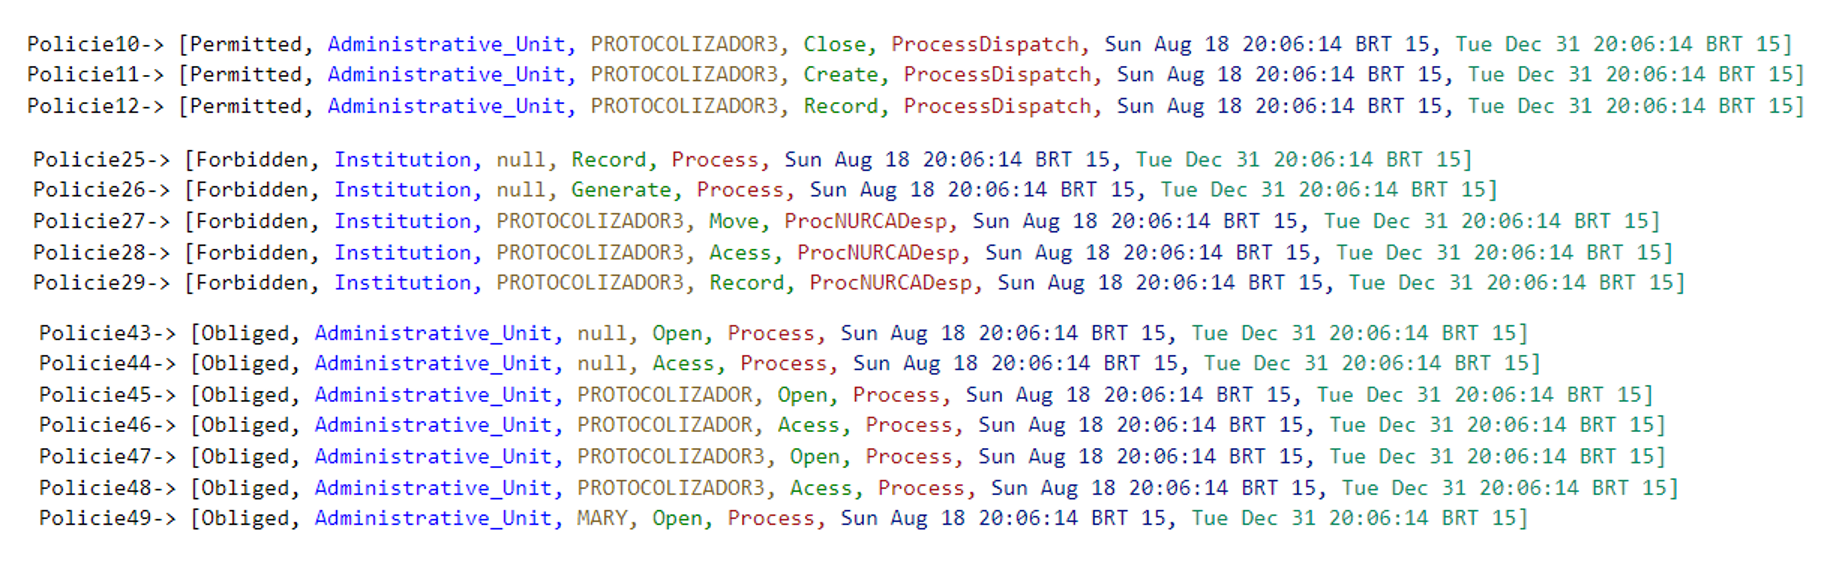
\includegraphics[width=1\textwidth]{imagens/modelo_politica.png}}
	
	{\scriptsize Fonte: compilação do autor}
	\label{fig:modelo_politica}
\end{figure}

Na próxima seção os conceitos de mineração de dados utilizado neste trabalho serão descritos.

\section{Mineração de Dados}\label{mineracao_dados}
Uma das características de nossa era é produção de dados em grande volume, velocidade e variedade de todas as formas, por dispositivos espalhados em toda parte. Entretanto, dados, mesmo em grande quantidade, são apenas dados. É preciso produzir informação e conhecimento para explorar as vantagens que essa massa pode trazer. O dado necessita ser, de alguma forma, analisado, tratado para que informações e conhecimento possam ser, deles, extraídos \cite{aprenda_mineracao_fernando_amaral16} \cite{ferrari2017}.

Conforme \citeonline{fayyad1996}:
\begin{citacao}
	 Os computadores permitiram que os humanos coletassem mais dados do que podemos digerir, é natural [,portanto,] recorrer a técnicas computacionais para nos ajudar a desenterrar padrões e estruturas significativas a partir dos numerosos volumes de dados. Por isso, [a mineração de dados] é uma tentativa de resolver um problema que a era da informação digital transformou em realidade para todos nós: sobrecarga de dados.
\end{citacao}

Para \citeonline{Boscarioli2017}, a \textit{mineração de dados} pode ser definida como um processo automatizado ou semiautomatizado de explorar grandes bases de dados de forma extensiva, com o objetivo de encontrar padrões relevantes que ocorrem nos dados e que sejam significativos para embasar a absorção de informação importante, contribuindo para a geração de conhecimento. 

Para \citeonline{fayyad1996}, o termo ``mineração de dados'' tem sido usado  por estatísticos, analistas de dados e comunidades de sistemas de informações ganhando popularidade no campo do banco de dados. Já o termo \textit{descoberta de conhecimento em bancos de dados [}(KDD, da sigla em Inglês)] foi cunhada para enfatizar que o conhecimento é o produto final de uma descoberta baseada em dados. Está sendo utilizado nos campos de IA e aprendizado de máquina.


\subsection{KDD - Knowledge Discovery in Databases}
Assim, a mineração de dados é parte integrante de um processo mais amplo, conhecido como descoberta de conhecimento em bases de dados (\textit{Knowledge Discovery in Databases}, ou \textit{KDD})\cite{fayyad1996}. 

Embora se use \textit{mineração de dados} como sinônimo de KDD, a terminologia é empregada para a etapa de \textit{descoberta}  do processo de KDD, que inclui a \textit{seleção} e \textit{integração} das bases de dados, a \textit{limpeza} da base, a \textit{seleção e transformação} dos dados, a \textit{mineração}(propriamente) e a \textit{avaliação} dos dados \cite{ferrari2017}\cite{Boscarioli2017}.

Assim, a mineração de dados  é definida em termos de esforços para a descoberta de padrões em bases de dados. A partir destes padrões descobertos, há condições de se gerar conhecimento útil para um processo de tomada de decisão (ou a geração de conhecimento para esta tomada).

Mais especificamente, KDD (\textit{Knowledge Discovery in Database}) é um processo de busca de conhecimento em bancos de dados e, de modo geral, consiste de uma sequência iterativa de passos (ou \textbf{etapas})\footnote{O processo de KDD, segundo \cite{fayyad1996} é composto por: \textit{Seleção de dados; Pré-processamento; Transformação; Mineração; Análise e assimilação de resultados}}: limpeza de dados; integração dos dados; seleção, transformação e mineração dos dados; avaliação dos padrões e apresentação e assimilação do conhecimento. Este processo é iterativo e, em alguma etapa, pode-se voltar para uma anterior \cite{Boscarioli2017}.

A \autoref{fig:processo-KDD} mostra o funcionamento iterativo do processo de KDD (\textit{Knowledge Discovery in Database}) -  Descoberta de Conhecimento em Bases de Dados.

\begin{figure}[h!]
	\centering
	\caption{Etapas do processo de descoberta do conhecimento em bases de dados - KDD}
	\fbox{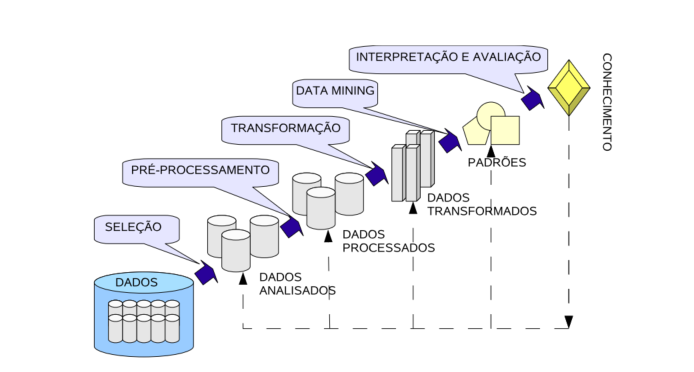
\includegraphics[width=1\textwidth]{imagens/processo-KDD.png}}
	
	{\scriptsize Fonte: \citeonline[p. 7]{vasconcelos_aplicacao_2018}}
	\label{fig:processo-KDD}
\end{figure}

Neste trabalho as tarefas de seleção e transformação dos dados farão parte da etapa chamada de pré-processamento de acordo com, \citeonline{Boscarioli2017} e serão descritas com maior riqueza de detalhes no \autoref{resultados}.

\subsection{Modelo de conhecimento}\label{modelo_conhecimento}
O termo \textbf{modelo de conhecimento} (ou hipótese) é utilizado na literatura (e neste trabalho) para fazer referência a um padrão ou conjunto de padrões descobertos (que é, enfim, o \textit{propósito} do processo de KDD). Estes padrões são conhecimentos representados segundo as normas sintáticas de alguma linguagem formal. Estes padrões podem ser classificados em dois tipos: \textit{preditivos} e \textit{descritivos} \cite{ferrari2017}.

O intuito dos preditivos é resolver um problema específico de prever os resultados ou valores de um ou mais atributos, em função dos valores de outros atributos. Os descritivos (ou informativos) tem o intuito de apresentar informações interessantes e importantes sobre os dados que um especialista de domínio possa não conhecer \cite{goldschmidt2005}. 

Modelos de conhecimento compostos exclusivamente por padrões preditivos são chamados de \textit{modelos preditivos}, enquanto que modelos descritivos são modelos de conhecimento compostos tão somente por padrões descritivos \cite{Boscarioli2017}.

Para \citeonline{minewiskan_modelos_nodate}, 
\begin{citacao}
	Um modelo de mineração é criado aplicando-se um algoritmo a dados, mas é mais que um algoritmo ou um contêiner de metadados: é um conjunto de dados, estatísticas e padrões que podem ser aplicados a novos dados para gerar previsões e fazer inferências sobre relações.
\end{citacao}

Neste contexto, este trabalho se concentra, portanto, em criar modelos de forma a detectar, mediante o uso de técnicas da mineração de dados (e aprendizagem de máquina) os conflitos entre as políticas de controle de acesso de um sistema. Diversos modelos serão desenvolvidos e confrontados usando-se vários algoritmos e técnicas analisados com métricas específicas.

\subsubsection{Arquitetura do modelo}\label{arquitetura_modelo}

Segundo \citeonline{minewiskan_modelos_nodate}, ``Um modelo de mineração obtém dados de uma estrutura de mineração e analisa esses dados usando um algoritmo de mineração de dados''. Entretanto, é importante diferenciar a estrutura e o modelo de mineração. Ainda de acordo com \citeonline{minewiskan_modelos_nodate}, a \textit{estrutura} armazena informações que definem a fonte de dados, já um \textit{modelo} de mineração armazena informações derivadas do processamento estatístico dos dados, como padrões encontrados em decorrência da investigação.

Assim, o modelo fica ``limpo'' até que os dados que foram guarnecidos pela estrutura de mineração sejam processados e avaliados. Depois de produzido o modelo contém \textit{metadados}, resultados e associações e pode, então, ser utilizado para a obtenção de conhecimento.

A arquitetura pode conter também, variáveis, \textit{hiperparâmetros}, definições do modelo, filtros utilizados e, claro, o algoritmo utilizado na tarefa de análise dos dados \cite{deep_learning_book_2019}.

\section{Aprendizagem de máquina} \label{aprendizagem_maquina}
Segundo \citeonline[p. 10]{goldschmidt2005}, 
\begin{citacao}
	um dos passos do processo de KDD, o de extração de padrões (ou Mineração de Dados) utiliza métodos de Aprendizado de Máquina (AM) [ou \textit{Machine Learning} - ML] para encontrar regularidades, padrões ou conceitos em conjuntos de dados.
\end{citacao}

A principal diferença, segundo os autores, \citeonline{goldschmidt2005} entre Aprendizagem de Máquina e KDD reside no fato de ``grande parte da literatura em AM se concentra apenas no mecanismo de descoberta de padrões e/ou conceitos, sem se preocupar com o grau de utilidade''. Já em KDD, ainda segundo \citeonline{goldschmidt2005}, ``os padrões extraídos são avaliados para aferir sua utilidade para o usuário em relação à tomada de decisão''. Ou seja, o aprendizado na Aprendizagem de Máquina é um atividade-fim enquanto o aprendizado no KDD é uma atividade-meio para a obtenção do conhecimento.

\subsection{Definição}
Aprendizado de máquina ou \textit{machine learning} é um braço da Inteligência Artificial que emprega técnicas e algoritmos na criação de modelos computacionais dos quais a característica principal é a capacidade de descobrir padrões em um grande volume de dados ou de melhorar o desempenho de uma determinada tarefa através da experiência (do \textit{reforço}) \cite{mohri_foundations_2018} \cite{alpaydin_introduction_2014} \cite{swamynathan_mastering_2019}

Então, de acordo com \citeonline[p. 278]{baeza-yates_recuperacao_2013}, ``os padrões aprendidos, que podem ser bem complexos, são então usados para fazer predições relativas a dados ainda não vistos e novos''.

Nas palavras de Arthur Lee Samuel \citeonline{wiederhold_arthur_1992}, considerado um dos pioneiros na área de inteligência artificial, aprendizado de máquina é ``o campo de estudo que dá aos computadores a capacidade de aprender sem serem explicitamente programado'' \cite[p. 89]{simon_too_2013}. 

Aprendizado de máquina tem sido aplicado na automatização de funções que para os humanos são executadas intuitivamente, mas que são difíceis de definir formalmente \cite{sarkar_2017}.

Assim, de forma geral, a aprendizagem de máquina tem por objetivo estudar e desenvolver métodos computacionais para obter sistemas capazes de adquirir conhecimento de forma automatizada \cite{lima_ia_2016}.

A capacidade de determinados algoritmos tem de aprender a partir de exemplos é chamado de \textbf{aprendizado indutivo}. Estes algoritmos aprendem relacionamentos eventualmente existentes entre os dados, mostrando o resultado nos modelos de conhecimento gerado \cite{goldschmidt2005} \cite{alpaydin_introduction_2014}.

Conforme \citeonline[p. 279]{baeza-yates_recuperacao_2013}, os algoritmos de aprendizado de máquina ``são fundamentalmente dependentes de uma fase de aprendizado, a qual é usada para produzir um modelo ou uma função que codifica padrões presentes nos dados de entrada''.

Então, dependendo de qual é a abordagem de aprendizado usada, os algoritmos de aprendizado de máquina podem ser, basicamente de 3 principais tipos, que são: a aprendizagem supervisionada, a aprendizagem não-supervisionada e a aprendizagem por reforço \footnote{Há ainda os tipos de aprendizado \textit{semissupervisionado} e a \textit{transdução} (ou inferência transdutiva) que não serão discutidos neste trabalho} \cite{Norvig2013} \cite{baeza-yates_recuperacao_2013}. 

Na \textbf{aprendizagem não-supervisionada} o modelo/hipótese busca padrões na entrada, embora não seja fornecido nenhum \textit{feedback} explícito. Portanto, na abordagem não-supervisionada não há, nos dados, uma classe, não há um rótulo prévio, ou seja, não existe a informação da saída desejada. O processo de aprendizado busca identificar regularidades entre os dados e não é necessária a divisão prévia dos dados em dados de treinamento, validação e teste.  A tarefa mais comum de aprendizagem não supervisionada é o agrupamento. mas, os algoritmos de aprendizagem não-supervisionada incluem ainda, modelos de redes neurais, análise de componentes independentes e o já citado \textit{clustering} (agrupamento) \cite{Norvig2013} \cite{Boscarioli2017} \cite{goldschmidt2005} \cite{aprenda_mineracao_fernando_amaral16}.

Na \textbf{aprendizagem supervisionada} o modelo/hipótese observa alguns exemplos de pares de entrada e saída, e aprende uma função (ou modelo) que faz o mapeamento entre a entrada e a saída. Portanto, ela compreende a abstração de um modelo a partir dos dados apresentados na forma de pares ordenados (\textit{entrada, saída, saída desejada}). Há, assim, uma \textit{classe}, ou um atributo especial com o qual se pode comparar e validar o resultado. Esta categoria de aprendizagem de máquina requer uma função de aprendizado dos dados de treinamento fornecidos como entrada. Esses dados, então, são usados para para aprender uma função de classificação que pode, assim, ser usada para realizar predições de classes para dados ainda não vistos ou novos \cite{Norvig2013} \cite{luger_inteligencia_2015} \cite{baeza-yates_recuperacao_2013}.

Na \textbf{aprendizagem por reforço}, aprende-se a partir de uma série de reforços --- recompensas ou punições. Não está disponível, geralmente, na aprendizagem por reforço, para o algoritmo de aprendizado de máquina, um conjunto de dados para treinamento. O aprendizado se dá, então, pela interação com o ambiente que se deseja atuar por um determinado período com o objetivo de melhorar o desempenho de uma determinada tarefa \cite{Norvig2013} \cite{aprenda_mineracao_fernando_amaral16} \cite{silva_restaurante_2019}.

\section{Algoritmos de classificação}
A classificação é considerada uma das tarefas principais do processo de aprendizagem de máquina, sendo, inclusive, a tarefa mais comum \cite{amaral_introducao_2018} \cite{fayyad1996}.

Segundo, \citeonline[p. 86]{amaral_introducao_2018}, ``Na classificação, os dados devem possuir uma \textit{classe} a qual queremos prever''. Conforme \citeonline{Rocha2012}, ``o termo \textit{classe} deve ser usado quando existe informação sobre quantas e quais são as partições presentes em um conjunto de dados, bem como qual exemplar pertence a qual partição''.

Comumente, denomina-se \textit{classificação} o processo pelo qual se determina uma função de mapeamento capaz de indicar a qual classe pertence algum exemplar de um domínio sob análise, baseando-se em um conjunto já classificado \cite{Boscarioli2017}.

Assim, de acordo com \citeonline{classification2013}, classificação é uma técnica de mineração de dados (aprendizado de máquina) usada para prever a associação ao grupo para instâncias de dados. É, segundo \citeonline{aprenda_mineracao_fernando_amaral16} e \citeonline{performance_classification2013}, como citado anteriormente, a tarefa mais utilizada em mineração de dados. Além de ser a mais complexa e a que possui a maior quantidade de algoritmos disponíveis, conforme descrito em \citeonline{classification2013}.

A classificação é uma das tarefas \textit{preditivas} de Mineração de Dados e aprendizado de máquina. Tarefas de predição consistem na análise de um \textit{dataset} (conjunto de dados), descritos por atributos e rótulos associados com o objetivo de descobrir um \textbf{modelo} capaz de mapear corretamente cada um dos dados a seus rótulos apropriadamente. Esse objetivo é alcançado por meio de técnicas, normmalmente, chamadas de supervisionadas. Este tipo de análise preditiva pode ser dividida em \textit{categórica}, também chamada de \textit{classificação} ou em \textit{numérica}, também chamada de regressão. Cf. \citeonline{Boscarioli2017}  e \citeonline{classification2013}, também exposto em \citeonline{ferrari2017} e \citeonline{goldschmidt2005}.

\underline{Formalmente}, a tarefa de classificação pode ser descrita como a busca por uma função de mapeamento para um conjunto $X$ de vetores de entrada (ou, exemplares --- os dados) $\vec{x_i} \in E^d$ para um conjunto finito de rótulos $C$ de cardinalidade $c$. A função $F$ é, então, definida como $F: E^d \times W \rightarrow C$, em que $d$ é a dimensão do espaço $E$, ou seja, a quantidade de coordenadas do vetor $\vec{x_i}$, e $W$ é um espaço de parâmetros ajustáveis por meio do algoritmo de indução supervisionada \cite{Boscarioli2017}.

Pode ser dividida em, ao menos, duas categorias: \textit{classificação binária} e \textit{classificação multiclasse}. Na binária, a cardinalidade $c$ é 2. Para o caso em que $c > 2$, o problema é considerado de múltiplas classes \cite{Boscarioli2017} \cite{classification2013}.

Os textos de \citeonline{classification2013}, \citeonline{performance_classification2013}, além dos de \citeonline{Wolpert:1996}, \citeonline{classification_survey2012} e \citeonline{using_data_mining2012}  trazem mais análises, técnicas, comparações e explicações mais aprofundadas de muitos algoritmos de classificação, entre eles, árvores de decisão, k-vizinhos mais próximos, Naive Bayes e Redes Bayesianas, Redes Neurais Artificiais, Máquinas de Vetores de Suporte (SVM) entre outros.   

\subsection{Teoria da aprendizagem e algoritmos de classificação }\label{sec:teoria_aprendizagem}
Sobre \textit{teoria da aprendizagem} e \textit{algoritmos de classificação} há uma discussão em \citeonline{Norvig2013} sobre qual seria, em relação às hipóteses de modelos de aprendizagem, aquela (ou aquelas) que melhor se ajuste aos dados futuros. Os autores citam a \textbf{\textit{suposição de estacionaridade}}, ou seja, que há uma distribuição de probabilidade sobre os dados que permanece estacionária ao longo do tempo. Supõe-se, portanto que cada exemplo de ponto de dados (antes de conhecê-lo) é uma variável aleatória $E_j$ cujo valor observado $e_j = (x_j, y_j)$ é amostrado da distribuição e é independente dos exemplos anteriores. 

Assim:
\begin{equation}
	P (E_j|E_{j-1},E_{j-2}, ... ) = P(E_j) \textrm{,} 
\end{equation}

e cada exemplo tem uma distribuição de probabilidade anterior idêntica:

\begin{equation}
P(E_j) = P(E_{j-1}) = P(E_{j-2}) = \dots 
\end{equation}

Estes exemplos são chamados de \textit{independentes e identicamente distribuídos} ou \textbf{i.i.d}. Esta suposição é, segundo os autores, \underline{necessária} para \textit{tentar a previsão sobre o futuro dos dados}. Há claro, ainda em \citeonline{Norvig2013}, um alerta sobre o fato de ser possível a aprendizagem ocorrer caso haja pequenas alterações (lentas) na distribuição.

Outro fato importante para a definição e avaliação da escolha da melhor hipótese (modelo) de um algoritmo de classificação é definir o ``melhor ajuste''. Em seu conhecido livro de Inteligência Artificial, os autores \citeonline{Norvig2013} definem a \textbf{taxa de erro} de uma hipótese como uma métrica importante para definir o ``melhor ajuste'' de um modelo/hipótese.

\subsection{Taxa de erro}\label{taxa_erro}
A taxa de erro é, assim, a proporção de erros que o algoritmo classificador comete --- a proporção de vezes que $h(x)\neq y$ para o exemplo $(x,y)$ --- sendo $h(x)$ a função que mapeia uma \textit{hipótese/modelo} $h$ com a \textit{previsão/valor} conhecido $y$. Nem sempre, como alerta, \citeonline{Norvig2013}, uma hipótese/modelo $h$ que tenha uma taxa de erro baixa no conjunto de treinamento generaliza bem e se comporta eficientemente para dados não conhecidos. A forma de testar o algoritmo é importante. Para isso há, na literatura, algumas técnicas que são utilizadas como estratégia de treinamento, validação e teste.

\subsection{Estratégias de validação}\label{estrategias_validacao}
Como citado por \citeonline{Norvig2013} e \citeonline{luger_inteligencia_2015} entre diversos autores e, cf. \citeonline[p. 125]{Boscarioli2017}, 
\begin{citacao}
	independentemente da medida de avaliação a ser usada para atestar a qualidade de um modelo, não é adequado avaliá-lo [apenas] por seu desempenho em relação aos exemplares apresentados no processo de treinamento (indução). É sempre necessário saber como o modelo se comporta quando aplicado a exemplares que ainda não conhece, ou seja, não usados no processo de sintonização de seus parâmetros.
\end{citacao}

Essa observação, claro, é porque modelos preditivos, dependendo de como são criados, podem levar ao \textit{\textbf{overfitting}} (sobreajuste). O fenômeno do sobreajuste ocorre, cf. \citeonline{Boscarioli2017} ``quando o modelo preditivo é gerado de forma a representar os exemplares usados para sua geração com uma fidelidade mais alta que o necessário''. 

Assim, modelos sobreajustados (ou superajustados) não são capazes de realizar predições adequadas para dados novos. Busca-se, na construção de modelos preditivos, uma maior \textit{generalização} e no caso do sobreajuste o fenômeno contrário ocorre. 

A maior causa de sobreajuste é quando os dados de treinamento não representam fielmente os dados novos (ou de produção) ou por serem diferentes (caso de dados antigos, por exemplo) ou por não serem significativos (poucos dados)\footnote{ é possível também o sobreajuste devido a \textit{ruídos} nos dados, pelo uso de um modelo de forma inapropriada ou de uma \textit{classe rara} \citeonline[p.35]{aprenda_mineracao_fernando_amaral16}}. A \autoref{fig:overfitting} mostra um modelo preditivo em que o lado direito representa um modelo sobreajustado e o lado esquerdo um modelo regularizado\footnote{As técnicas de \textbf{\textit{regularização}} são usadas para reduzir o overfitting. As técnicas mais utilizadas são o decaimento de pesos (weight decay) ou regularização L2 e o custo quadrático. \cite{deep_learning_book_2019}.} para o mesmo \textit{dataset}.

\begin{figure}[h!]
	\centering
	\caption{Modelo sobreajustado e regularizado para o mesmo \textit{dataset}.}
	\fbox{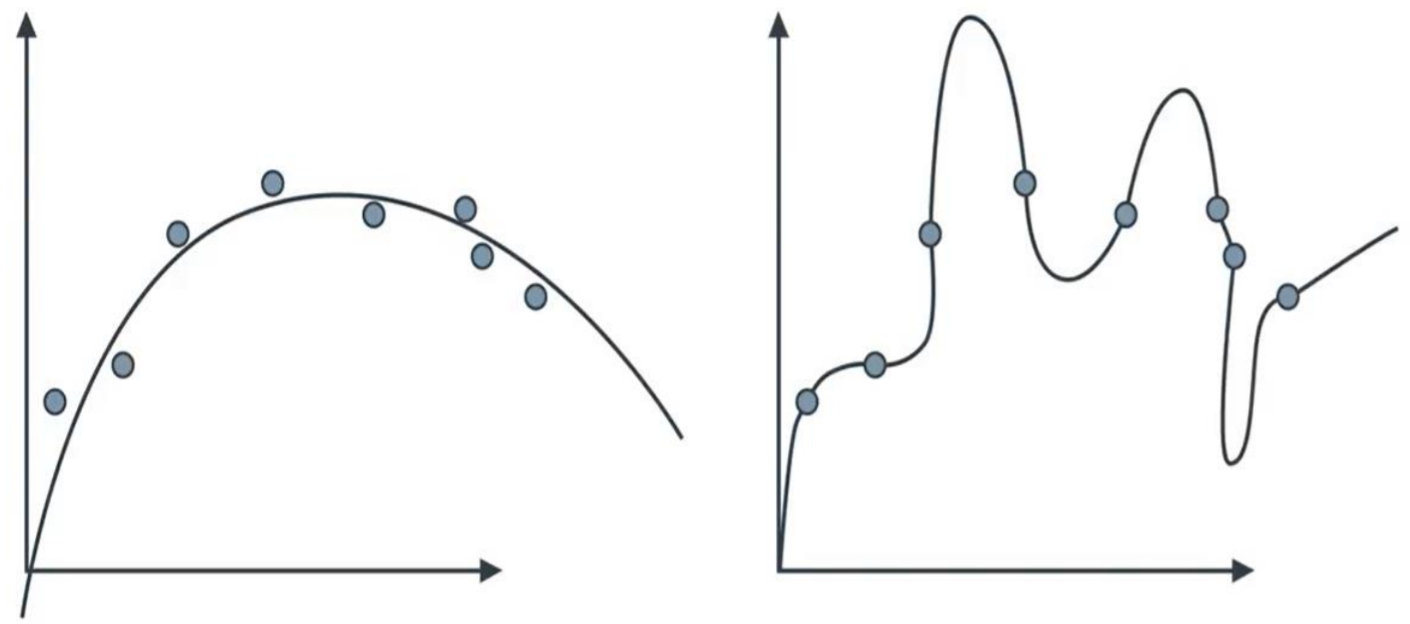
\includegraphics[width=.6\textwidth]{imagens/overfitting.png}}
	
	{\scriptsize Fonte: baseado no encontrado em \citeonline{over_and_underfitting_2019}}
	\label{fig:overfitting}
\end{figure}

Nas palavras de \citeonline[p. 95]{amaral_introducao_2018}, ``o processo de construção de um modelo de aprendizado de máquina busca, obviamente, maximizar a precisão e minimizar a taxa de erros''. Para tanto, a literatura cita diversas técnicas e estratégias para a avaliação de modelos preditivos. Autores diversos, como \citeonline{Boscarioli2017}, \citeonline{aprenda_mineracao_fernando_amaral16}, além de  \citeonline{data_science_do_zero2016} e \citeonline{ferrari2017} citam, geralmente, como estratégia de treinamento, validação e teste as seguintes técnicas:
\begin{itemize}
	\item Resubstituição;
	\item Holdout;
	\item Validação cruzada;
	\item Bootstrap;
\end{itemize}
Na \textbf{\underline{resubstituição}}, segundo \citeonline{Boscarioli2017}, as medidas de avaliação dos classificadores são aplicadas no próprio conjunto de dados usados para indução do modelo. Essa técnica, embora tenha alguns vantagens discutidas em \citeonline{ferrari2017} e \citeonline{Boscarioli2017}, pode levar ao, já citado, sobreajuste (\textit{overfitting}) e é discutido em \citeonline{data_science_do_zero2016}, também em \citeonline{aprenda_mineracao_fernando_amaral16} e \citeonline{Norvig2013}. Como já afirmado anteriormente, o sobreajuste é quando se produz um modelo de bom desempenho com os dados de treinamento, mas que não lida bem com novos dados.

Na técnica de \textbf{\underline{Holdout}}, pressupõem-se uma divisão, ou criação de dois subconjuntos de dados distintos, a partir do conjunto de dados disponível pra uso na indução do modelo/hipótese. Um desses subconjuntos será usado para treinamento (indução) do modelo de previsão e o segundo, para teste após o término do treinamento e, consequentemente, na aplicação das medidas de avaliação do modelo/hipótese \cite{Boscarioli2017}

A \autoref{fig:img_holdout} mostra o funcionamento da técnica de holdout de forma mais detalhada.
\begin{figure}[h!]
	\centering
	\caption{Funcionamento da técnica holdout.}
	\fbox{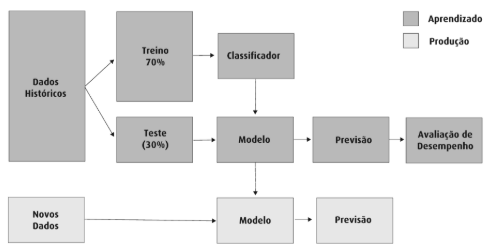
\includegraphics[width=.6\textwidth]{imagens/hold_out.png}}
	
	{\scriptsize Fonte:\cite{aprenda_mineracao_fernando_amaral16}}
	\label{fig:img_holdout}
\end{figure}

Na estratégia de \textbf{\underline{validação cruzada}}, todos os dados farão parte, em algum momento, do conjunto de dados usado no teste do modelo/hipótese. A ideia é que cada exemplo sirva duplamente --- como dados de treinamento e dados de teste. Primeiro divide-se o conjunto em $k$ subconjuntos iguais. Em seguida realiza-se $k$ rodadas de aprendizagem; em cada iteração $\frac{1}{k}$ dos dados é retido como conjunto de teste e os exemplos restantes são usados como treinamento. 

Valores populares de $k$ são 5 e 10 --- o suficiente para uma estimativa estatisticamente provável que seja precisa a um custo 5-10 vezes maior no tempo de computação. Há também o extremo do $k = n$, também conhecido como \textbf{validação cruzada com omissão de um}. O método de validação cruzada permite que o modelo/hipótese seja avaliado uma série de vezes, cada série sendo conhecida como partição (ou \textit{fold}). Ao final, a avaliação pode ser realizada aplicando medidas estatísticas como média, desvio-padrão e intervalo de confiança ao conjunto de $k$ avaliações obtidas ou somando-se os desempenhos obtidos pelos $k$ modelos gerados e dividindo essa soma pelo número de exemplares original \cite{Norvig2013}\cite{Boscarioli2017}\cite{ferrari2017} \cite{aprenda_mineracao_fernando_amaral16}.

A \autoref{fig:img_cross_validation} mostra um exemplo didático de como funciona a validação cruzada. Os dados que não fazem parte do conjunto de teste em cada rodada são utilizados no treinamento.

\begin{figure}[h!]
	\centering
	\caption{Funcionamento da técnica \textit{cross validation}}
	\fbox{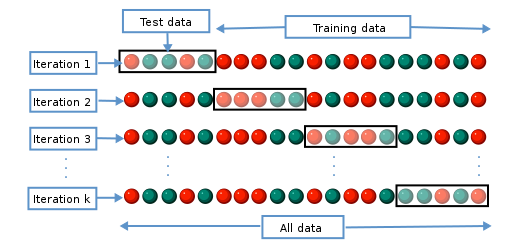
\includegraphics[width=.6\textwidth]{imagens/cross_validation.png}}
	
	{\scriptsize Fonte: \cite{fold_cross_validation:k-fold_nodate}}
	\label{fig:img_cross_validation}
\end{figure}

Já a técnica de \textit{\textbf{\underline{Bootstrap}}} funciona de forma  parecida à estratégia \textit{holdout}. Ela também usa dois conjuntos, um de treinamento e outro para teste, porém durante o processo de formação dos subconjuntos, exemplares que já foram sorteados podem novamente serem contemplados, com probabilidade igual. É uma estratégia que permite, portanto, a reposição.

Neste trabalho, todos os algoritmos de classificação usados foram testados usando as técnicas de resubstituição, \textit{holdout} (com taxas de 70-30, 75-25 e 60-40), além de \textit{cross-validation} com 3, 5 e 10 folds. 

Como explicado em \citeonline{WolpertMacready} e \citeonline{Wolpert:1996} não existe um algoritmo de aprendizado superior a todos os demais quando considerados todos os problemas de classificação possíveis (teorema \textbf{NFL}, ou \textit{No Free Lunch}), portanto, variações foram executadas nos experimentos em todas técnicas avaliadas, alterando-se os padrões para chegar a métricas e medidas de avaliação mais eficientes.

\subsubsection{Medidas de avaliação}\label{medidas_avaliacao}

Para \citeonline{castro_supervised_2011}, 
\begin{citacao}
	Tradicionalmente, a métrica usada na avaliação e seleção de modelos de classificação é a acurácia (ou taxa de erro) estimada em relação a um dado conjunto de teste. Essa metodologia é justificada pela formulação padrão do problema do aprendizado supervisionado que visa a minimização da probabilidade do erro global. 
\end{citacao}

Há, porém, conforme \citeonline{Boscarioli2017}, \citeonline{aprenda_mineracao_fernando_amaral16}, \citeonline{classification2013} e \citeonline{classification_survey2012} diversas medidas usadas na avaliação de classificadores. 

A que será usada neste trabalho (com o objetivo de minimizar a probabilidade do erro global) é a, já citada, acurácia ou taxa de classificações corretas. 

A métrica acurácia é dada, portanto, por:

\begin{equation}\label{acuracia}
	\textrm{Acurácia} = |y-f(\aleph)=0|\textrm{,}
\end{equation}

em que $|equação|$ representa a contagem de vezes em que $equação$ é verdadeiro, $f$ é o modelo preditivo, $\aleph$ é o subconjunto de dados sob o qual o modelo está sendo avaliado, $f(equação)$ é a classificação fornecida pelo modelo preditivo para cada um dos exemplares (dos dados), e $y$ é a classe esperada como resposta cf. \citeonline[p. 129]{Boscarioli2017}.

A acurácia de um classificador também pode ser descrita em termos do \textbf{erro de generalização} $\xi_g$, e uma função de perda binária e, portanto, ser interpretada como a probabilidade de ocorrer uma classificação correta. Dessa forma:

\begin{equation}
\textrm{Acurácia}_g=1 - \xi_g
\end{equation}

Ou seja, a acurácia é, basicamente o número de acertos (positivos) divido pelo número total de exemplos. Será a métrica mais usada para avaliar os classificadores neste trabalho.

Há, entretanto, em modelos preditivos que trabalham com dados numéricos (como as redes neurais e o SVM), pode-se utilizar uma função de perda contínua, capaz de medir o erro entre a resposta obtida pelo modelo preditivo e a resposta aguardada \cite{Boscarioli2017} \cite{deep_learning_book_2019}.

A função de perda também é conhecida, popularmente, como função de custo. Basicamente ela é a diferença entre os valores de rótulo de treinamento e a previsão feita pelo modelo. Os parâmetros do modelo devem, assim, serem estimados em relação à minimização da função de perda. Classificadores diferentes podem ser configurados com funções de perda diferentes.  \cite{nn_smithing_1999} \cite{minewiskan_modelos_nodate} \cite{silva_redes_2016} \cite{Boscarioli2017} \cite{goldschmidt2005} \cite{geron_maos_2020} \cite{deep_learning_book_2019}

Para \citeonline{nn_smithing_1999}
\begin{citacao}
	A função de custo reduz todos os aspectos bons e ruins de um sistema complexo a um único número, um valor escalar, o que permite ranquear e comparar as soluções candidatas.
\end{citacao}

Algumas funções de perda (\textit{loss functions}), comuns, neste contexto são, de acordo com \citeonline{Boscarioli2017}:

\begin{equation}\label{erro_absoluto}
	\textrm{\textit{Erro absoluto}}=\sum_{<\vec{x}_i, y_i> \in \aleph} |y_i - f(\vec{x}_i)|
\end{equation}

\begin{equation}\label{erro_quadratico}
\textrm{\textit{Erro quadrático}}=\sum_{<\vec{x}_i, y_i> \in \aleph} (y_i - f(\vec{x}_i))^2
\end{equation}

\begin{equation}\label{erro_absoluto_medio}
\textrm{\textit{Erro absoluto médio}}=\sum_{<\vec{x}_i, y_i> \in \aleph} |y_i - f(\vec{x}_i)|/m
\end{equation}

\begin{equation}\label{erro_quadratico_medio}
\textrm{\textit{Erro médio quadrático}}=\sum_{<\vec{x}_i, y_i> \in \aleph} (y_i - f(\vec{x}_i))^2/m
\end{equation}

Onde $m$ é a quantidade de instâncias existentes em $\aleph$. 

\citeonline{Boscarioli2017}, \citeonline{amaral_introducao_2018} além de \citeonline{deng_improved_2016} e \citeonline{ruuska_evaluation_2018} afirmam que é importante analisar o tipo de erro que o modelo está cometendo e, principalmente, no caso de classificadores binários, é possível observar que, mesmo com uma acurácia alta o classificador pode não estar respondendo de forma adequada. 

Para realizar esse tipo de análise, os autores citados no princípio deste parágrafo, citam que uma ferramenta adequada é a \textit{\textbf{matriz de confusão}}. 

Geralmente, uma matriz de confusão tem dimensões $C \times C$, em que $C$ é o número de classes presentes no problema de classificação que está sendo avaliado. As linhas dessa matriz são indexadas seguindo as ``classes esperadas'' $(y)$, e as colunas seguindo as ``classes preditas'' $(f(x) ou \hat{y})$. 

Cada célula é um contador que é incrementado a depender do resultado da comparação de $f(x)$ e $y$. As respostas corretas do modelo geram os valores que entram na diagonal principal da matriz \cite[p. 130]{Boscarioli2017}.

A \autoref{fig:matriz_confusao} demonstra o procedimento de preenchimento de uma matriz de confusão conforme a resolução de um problema hipotético de classificação.

\begin{figure}[h!]
	\centering
	\caption{Preenchimento de uma matriz de confusão}
	\fbox{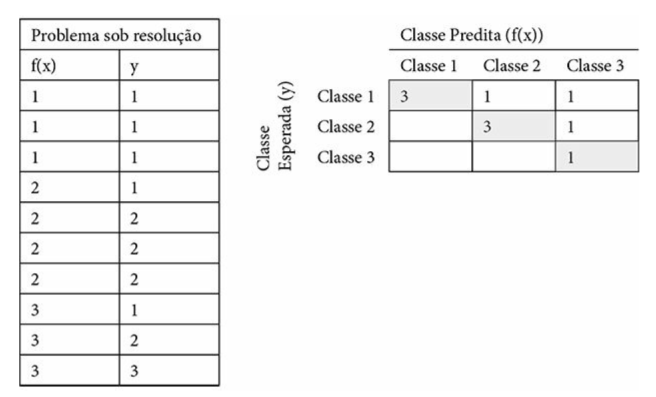
\includegraphics[width=.8\textwidth]{imagens/confusion_matrix.png}}
	
	{\scriptsize Fonte: \citeonline[p. 130]{Boscarioli2017}}
	\label{fig:matriz_confusao}
\end{figure}

Matrizes de confusão são, cf. \citeonline{ruuska_evaluation_2018} e \citeonline{Boscarioli2017}, particularmente úteis para avaliação de classificadores binários. Neste caso, os valores são atribuídos conforme ilustrado na figura (neste caso, as duas classes estão definidas como ``classe positiva'' e ``classe negativa''). 

\begin{figure}[h!]
	\centering
	\caption{Matriz de confusão para o caso de um classificador binário}
	\fbox{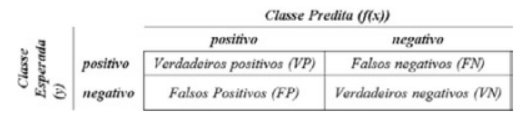
\includegraphics[width=0.8\textwidth]{imagens/matriz_confusao_binario.png}}
	
	{\scriptsize Fonte: \citeonline[p. 131]{Boscarioli2017}}
	\label{fig:binario_matriz_confusao}
\end{figure}

Cada célula, neste caso, possui o seguinte significado:

\begin{itemize}
	\item Verdadeiro Positivo (VP): classificação correta na classe positiva. A instância pertence a classe positiva e o modelo classificou na classe positiva.
	\item Falso Positivo (FP): classificação incorreta na classe negativa. A instância pertence à classe negativa, mas o classificador a classificou como pertencente à classe positiva.
	\item Verdadeiro Negativos (VN): classificação correta na classe negativa. A instância pertence a classe negativa e o modelo classificou na classe negativa.
	\item Falso Negativo (FN): classificação incorreta na classe negativa. classificação incorreta na classe negativa. A instância pertence à classe positiva, mas o classificador a classificou como pertencente à classe negativa. 
\end{itemize}

Os algoritmos que serão descritos nas próximas seções foram escolhidos neste trabalho porque foram descritos por \citeonline{wu2007} como alguns dos principais na área da Mineração de Dados e são reconhecidos por serem utilizados em diversos outros trabalhos.

\section{Naïve Bayes}\label{sec:naive-bayes}
Os algoritmo Naïve Bayes é um classificador probabilístico baseado na aplicação do Teorema de Bayes\footnote{Criado por Thomas Bayes (1701-1761), usa a probabilidade condicional que é a probabilidade de se observar algum evento (por exemplo $X = i$) dado algum outro evento (por exemplo, $Y=i$), escrito como $P(X_i|Y_i)$ \cite{bruce_estatistica_2019}}. É um dos mais utilizados em tarefas de classificação por apresentar bom desempenho em problemas de classificação tanto com dados categóricos quanto com dados numéricos. \cite{Boscarioli2017} \cite{amaral_introducao_2018} \cite{goldschmidt2005} \cite{bruce_estatistica_2019}.

Recebe o nome de ``ingênuo'' (naïve) porque ele considera como hipótese que os atributos previsores são \textit{estaticamente independentes} entre si, o que, em muitos casos práticos, não ocorre. Entretanto, a prática mostra que o classificador é efetivo mesmo em casos em que os atributos previsores não são estaticamente independentes. \cite{Boscarioli2017} \cite{goldschmidt2005} \cite{bruce_estatistica_2019}.

Portanto, o Naïve Bayes usa a probabilidade de observação dos valores previsores, dado um resultado, para estimar a probabilidade de observar o resultado $Y = i $, dado um conjunto de valores preditores. Usa a probabilidade posterior que é a probabilidade de um resultado após a informação preditora ter sido incorporada.

A classificação usando o algoritmo Naïve Bayes funciona da seguinte forma (usando todo o conjunto de dados para prever os resultados) \cite{bruce_estatistica_2019}:
\begin{enumerate}
	\item Para uma resposta bynária $ Y = i$ (i = 0 ou 1), é estimada as probabilidades condicionais individuais para cada preditor $  P(X_j | Y) = i $; estas são as probabilidades de o valor previsor estar no registro quando se observa $ Y = i $. Essa probabilidade é estimada pela proporção de valores $ X_j $ entre os registros $ Y = i $ no conjunto de treinamento;
	\item Essas probabilidades são multiplicadas uma pela outra, e então pela proporção de registros pertencentes a $ Y = i $;
	\item Os passos 1 e 2 são repetidos para todas as classes;
	\item É estimado uma probabilidade para o resultado $ i $ assumindo o valor calculado no passo 2 para cada classe $ i $ e dividindo-o pela soma de tais valores para todas as classes;
	\item É atribuído o registro à classe com a maior probabilidade para esse conjunto de valores preditores.
\end{enumerate}

O algoritmo pode, também, ser escrito como uma equação para a probabilidade de se observar um resultado $ Y = i $, dado um conjunto de valores previsores $ X_1, \cdots, X_p $:

\begin{equation}\label{eq:prob-naive-bayes}
  P(X_1, X_2, \cdots, X_p)
\end{equation} 

O valor da \autoref{eq:prob-naive-bayes} é um fator de escalonamento para a garantia de que a probabilidade esteja entre 0 e 1 e não dependa de:

\begin{eqnarray}
P(X_1, X_2, \dots, X_p)=P(Y&=&0)(P(X_1 | Y = 0)P(x_2 | Y = 0) \dots P(X_p| Y = 0)) + P(Y=1)\nonumber\\
(P(X_1 | Y = 1)P(X_2 | Y = 1) &\dots &P(X_p | Y = 1))\end{eqnarray}

Segundo \citeonline{bruce_estatistica_2019}, o Naïve Bayes ``é conhecido por produzir estimativas \textit{enviesadas}.No entanto, no que o objetivo seja \textit{ordenar} os registros conforme a probabilidade de $ Y = 1 $, as estimativas de probabilidade não enviesdas não são necessária'' e o classificador produz bons resultados.

\section{K-NN --- K-vizinhos mais próximos}\label{sec:knn}
O algoritmo KNN, ou \textit{\textbf{k-vizinhos mais próximos}} é um método de classificação supervisionada que serve para estimar a função de densidade $ F(x/C_j) $ dos atributos previsores $ x $ para cada classe $ C_j $. É um método estatístico não-paramétrico\footnote{o termo estatística não-paramétrica designa-se a estatísticas que não possuem dados ou população com estruturas ou parâmetros característicos ou é definido como uma função de uma amostra que não tem dependência de parâmetros \cite{bruce_estatistica_2019}}. \cite{Boscarioli2017} \cite{goldschmidt2005}

É usado para classificação e regressão. Ele estima o valor da função de densidade de probabilidade diretamente da probabilidade \textit{a posteriori} de que um elemento $x$ pertença a uma classe $C_j$ a partir da informação proporcionada pelo conjunto de treinamento. \cite{Boscarioli2017} \cite{bruce_estatistica_2019}.

No processo de aprendizagem, nenhuma suposição é feita sobre a distribuição das variáveis previsoras (por isso ele é \textit{não-paramétrico}). \cite{Boscarioli2017} \cite{goldschmidt2005} \cite{wu2007} \cite{bruce_estatistica_2019}. 

É um estilo de processamento conhecido como ``avaliação preguiçosa'' (\textit{lazy evaluation}) já que não existe um trabalho prévio de análise e construção de um modelo de classificação (pois o mesmo é baseado nas instâncias existentes --- o que pode, dispender muito tempo dependendo do tamanho do \textit{dataset} (conjunto de dados) disponível para o treinamento. \cite{Boscarioli2017}.

Segundo \cite{goldschmidt2005}, ``o K-NN considera que os registros do conjunto de dados correspondem a pontos no $R^n$, em que cada atributo corresponde a uma dimensão deste espaço''.

E prossegue: \citeonline[p. 117 e 118]{goldschmidt2005}
\begin{citacao}
	No método k-NN, o conjunto de dados é armazenado. Quando um novo registro deve ser classificado, este registro é comparado a todos os registros do conjunto de treinamento para identificar $k$ vizinhos mais próximos, \textit{i.e.}, mais semelhantes, de acordo com alguma métrica. A classe do novo registro é determinada por inspeção das classes desses vizinhos mais próximos, de acordo com a métrica selecionada. A resposta do método é a classe mais frequente entre os vizinhos mais próximos.
\end{citacao}	

É, desta forma, um aprendizado baseado em instâncias (\textit{instance-based learning}) já que a classificação de um exemplar cuja classe é desconhecida é realizada a partir da comparação desse exemplar com aqueles que possuem uma classe já conhecida. \cite[p. 80]{Boscarioli2017}. A padronização (mostrada em \autoref{eq:padronizacao}) pode melhorar consideravelmente a exatidão e precisão do algoritmo. \cite{bruce_estatistica_2019}.


Os exemplos de treinamento são vetores em um espaço de característica multidimensional, cada exemplo é descrito em termos de $p$ atributos considerando $q$  classes para classificação. Os valores de atributo para a  $i$-ésimo instância (onde $1 \leq i \leq n$) são representados pelo vetor $p$-dimensional: \cite{bruce_estatistica_2019} \cite{alpaydin_introduction_2014} \cite{classification2013}.

\begin{equation}
x_{i}=(x_{1i},x_{2i},...,x_{pi})\in X
\end{equation}

Embora o processo possa ser custoso, dependendo do tamanho do conjunto de dados de treinamento, a lógica que o implementa é simples: \cite{Boscarioli2017} \cite{bruce_estatistica_2019} \cite{goldschmidt2005}

Considerando um conjunto de dados de um problema de classificação e um novo registro a ser classificado. Considere também que foi definido um valor para a quantidade de vizinhos a ser examinada, ou seja, o valor do parãmetro $ k $. Sendo assim, o algoritmo k-NN segue os passos subsequentes:
\begin{enumerate}
	\item Cálculo da distância da nova instância (do novo registro) para cada uma das instâncias existentes no conjunto de dados;
	\item Identificação daquelas $k$ instâncias do conjunto de dados que apresentaram a menor distância em relação ao novo registro (ou seja, os mais similares);
	\item Verificação da classe mais frequente entre os $ k $ registros identificados no passo anterior;
	\item Atribuir à nova instância esta classe.
\end{enumerate}

Há, na literatura, várias formas de medir distâncias entre duas instâncias sendo a escolha de qual usar variando de acordo com o problema. As principais métricas de distância são: \cite{Boscarioli2017} \cite{alpaydin_introduction_2014} \cite{classification2013}
\begin{itemize}
	\item Euclidiana;
	\item Minkowsky;
	\item Chebishev;
	\item Manhattan.
\end{itemize}

A distância Euclidiana é dada por:
\begin{equation}\label{eq:euclidiana}
D_E(p,q) = \sqrt{(p_1 - q_1)^2 + \dots + (p_n - q_n)^2} = \sqrt{\sum_{i=1}^n (p_i - q_i)^2}
\end{equation}
É a mais utilizada por representar a distância física entre pontos em um espaço $d$-dimensional.

A de Minkowski é dada por:
\begin{equation}\label{eq:minkowiski}
D_M(p,q) =  \Big(\sum_{i=1}^n |p_i-q_i|^r \Big) ^\frac{1}{r}
\end{equation}
A distância de Minkowski é uma métrica para o espaço Euclidiano que serve de generalização para outras distâncias, como a própria Euclidiana e a Manhattan. 

A distância de Chebyshev é dada por:
\begin{equation}\label{eq:chebyshev}
D_C(p,q) = max_i(|p_i, q_i|)
\end{equation}

E a de Manhattan é dada por:
\begin{equation}\label{eq:manhattan}
D_M(p,q) = \sum_{i}^{n} \big| p_i - q_i \big| 
\end{equation}

Nestes casos, $ p = (p_1, \dots, p_n)$ e $ q = (q_1, \dots, q_n) $ representam dois pontos $n$-dimensionais e na \autoref{eq:minkowiski}, $r$ é uma constante.

\begin{figure}[h!]
	\centering
	\caption{Exemplo do algoritmo k-NN}
	\fbox{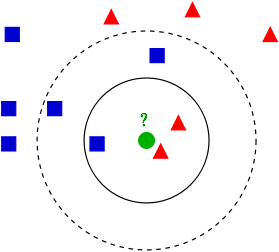
\includegraphics[width=0.5\textwidth]{imagens/KnnClassification-svg.png}}
	
	{\scriptsize Fonte: distribuído sob GPL no endereço: \href{https://bit.ly/3oKQLE1}{https://bit.ly/3oKQLE1} }
	\label{fig:k-nn}
\end{figure}

No exemplo da \autoref{fig:k-nn},  a instância a ser classificada é o círculo verde. Para $k = 3$, o círculo verde seria classificado com a classe do triângulo, pois há apenas um quadrado e 2 triângulos, dentro do círculo que os contém. Se k = 5 será classificado com a classe quadrada, pois há 2 triângulos e 3 quadrados, dentro do círculo externo. Neste exemplo, as distâncias mostradas na \autoref{eq:euclidiana}, na \autoref{eq:chebyshev}, na \autoref{eq:minkowiski} e na \autoref{eq:manhattan} seriam calculados entre o círculo verde e todas as outras figuras (instâncias). Este exemplo é 2D, logo, cada ponto teria seu valor em $x$ e em $y$. Para dimensões maiores a abordagem é a mesma, contudo, a visualização das amostras no espaço é um pouco mais complicada. \cite{Boscarioli2017} \cite{data_science_do_zero2016} \cite{goldschmidt2005}.

A escolha de $k$ depende dos dados. Geralmente, grandes valores de $k$ reduzem o efeito do ruído na classificação, mas criam limites entre classes semelhantes. Um bom $k$ pode ser selecionado através de otimização. O caso especial em que se prevê que a classe seja a classe mais próxima do exemplo de treinamento (quando  $k = 1$) é denominado Algoritmo do Vizinho Mais Próximo. 

Na próxima seção serão descritos alguns conceitos envolvendo as RNA's, Redes Neurais Artificiais.

\section{Redes Neurais Artificiais - RNA}
As redes neurais instituem um campo da ciência da computação, parte da área da inteligência artificial, que busca efetivar modelos matemáticos que se assemelhem às redes neurais biológicas. Elas apresentam capacidade de adaptar seus parâmetros como resultado da interação com o meio externo \cite{ferneda_redes_2006}\cite{Norvig2013}.

\subsection{Definição}

Para \citeonline[p. 41]{santos_um_2013} 
\begin{citacao}
	Uma rede neural artificial consiste de um sistema composto por neurônios dispostos em camadas, interligados através de pesos sinápticos construindo um sistema que simula o cérebro humano, inclusive seu comportamento. E uma técnica computacional que apresenta um modelo inspirado na estrutura neural de organismos inteligentes e que adquire conhecimento através da experiência.
\end{citacao}

De acordo com \citeonline[p. 47]{lima_ia_2016}, ``redes neurais podem ser caracterizadas como modelos computacionais com capacidades de adaptar, aprender, generalizar, agrupar ou organizar dados''.

Inicialmente, portanto, se desenvolveram como uma estratégia de simular os processos mentais humanos, como reconhecimento de imagens e sons, e após, como instrumento tecnológico e eficiente para muitas tarefas \cite{jin_development_2002}.	

Para \citeonline{obaidat_multilayer_1994}, as redes neurais artificiais podem ser usadas efetivamente para prover soluções para um amplo espectro de aplicações, incluindo mapeamento de padrões e classificação, análise e codificação de imagens, processamento de sinais, otimização, manipulação de grafos, reconhecimento de caracteres, reconhecimento automático de alvo,  	fusão de dados, processamento de conhecimento, controle de qualidade, mercado de ações, processamento de hipotecas, triagem de créditos para empréstimos entre muitos outros problemas. 

\subsection{Modelo de neurônio artificial}\label{perceptron}
Desde a década de 1940 com o trabalho de \citeonline{mcculloch_logical_1943} que se busca um modelo computacional que simule o cérebro humano e suas conexões. O interesse pela pesquisa nesta área cresceu e se desenvolveu durante os anos 50 e 60. É dessa época que \citeonline{rosenblatt_perceptron:_1958} sugeriu um método de aprendizagem para as redes neurais artificiais chamado \textit{perceptron}. 

Até o final da década de 1960 muitos trabalhos foram feitos usando o percepton como modelo, mas ao final desta década, \citeonline{minsky_perceptrons:_1969} apresentaram significativas limitações do perceptron. 

A pesquisa diminui consideravelmente nos anos seguintes (o chamado inverno da IA), porém durante  os  anos  80,  a excitação	ressurge mediante os avanços metodológicos importantes e, também, ao aumento dos recursos computacionais disponíveis. O  modelo  de  neurônio  artificial  da \autoref{fig:neuronio} é uma simplificação do apresentado por \citeonline[p. 36]{haykin_redes_2001}.

\begin{figure}[h!]
	\centering
	\caption{Modelo matemático de um neurônio}
	\fbox{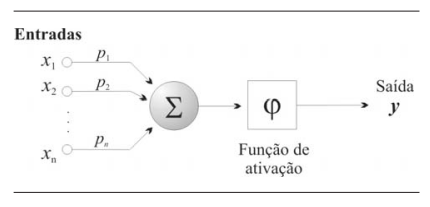
\includegraphics[width=.7\textwidth]{imagens/modelo_matematico_neuronio.png}}
	
	{\scriptsize 	Fonte: \citeonline[p. 36]{haykin_redes_2001}}	
	\label{fig:neuronio}
\end{figure}

O modelo da \autoref{fig:neuronio} é composto por três elementos:

\begin{itemize}
	\item  um conjunto de $ n $ conexões de entrada ($ x_1, x_2, \dots , x_n $), caracterizadas por pesos ($ p_1, p_2, \dots, p_n $);
	\item um somador ($ \sum $) para acumular os sinais de entrada;
	\item uma função de ativação ($\varphi$) que, no caso específico do neurônio apresentado por McCullock-Pitts em \citeonline{mcculloch_logical_1943} é uma função de limiar \cite{ferneda_redes_2006} \cite{lima_ia_2016}.
\end{itemize}

O comportamento das conexões entre os neurônios é simulado através de seus pesos  ($ p_1, p_2, ..., p_n $). Os valores podem ser positivos ou negativos (dependendo se a conexão é \textit{inibitiva} ou \textit{excitativa}. 

O efeito de um sinal proveniente de um neurônio é determinado pela multiplicação do valor do sinal recebido pelo peso da conexão correspondente ($x_i \times p_i$).

Então é efetuada a soma dos valores $x_i \times p_i$ de todas as conexões e o valor resultante é enviado para a função de ativação que define a saída ($y$) do neurônio. cf. \citeonline{Norvig2013} e \citeonline{mcculloch_logical_1943}, além de \citeonline{minsky_perceptrons:_1969}, \citeonline{ferneda_redes_2006} e \citeonline{haykin_redes_2001}

Matematicamente, a saída $y_k$ do neurônio mostrado na \autoref{fig:neuronio} é dada pela expressão abaixo:
\begin{equation}
	Y_k = \varphi(u_k) \qquad \textrm{onde} \qquad u_k = \sum_{i=1}^{n} P_{ki}X_i 
\end{equation}

A função de ativação proposta inicialmente por McCullock e Pitts em seu trabalho seminal, \citeonline{mcculloch_logical_1943} é uma função de limiar:

\begin{equation}\label{funcao_limiar}
y_k = \varphi (u_k) = \left \{ \begin{matrix}
									1, & \mbox{se }u_k > 0 \\ 
									0, & \mbox{se }u_k < 0 
								\end{matrix} 
							\right.
\end{equation}

Uma alteração importante neste modelo foi a introdução de um parâmetro polarizador (\textit{bias} ou \textit{offset}) $b_k$, conforme a \autoref{fig:bias_neuronio} cujo objetivo é deslocar o valor da informação referente à entrada líquida $u_k$, de forma a verter a função de ativação no eixo correspondente ao valor de $u_k$. Assim a saída $y_k = \varphi(u_k)$.

\begin{figure}[h!]
	\centering
	\caption{Adição de um \textit{offset} (\textit{bias}) no modelo do neurônio}
	\fbox{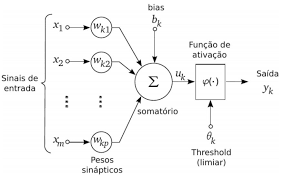
\includegraphics[width=.6\textwidth]{imagens/bias_neuronio.png}}	
	
	{\scriptsize 	Fonte: \citeonline[p. 58]{lima_ia_2016}}
	\label{fig:bias_neuronio}
\end{figure}

Dessa forma, o polarizador (bias) pode ser tratado como mais um peso da rede. Basta considerar um nova entrada do tipo $x_0 = 1$, com um peso associado $w_0 = b_k$, assim a representação fica sendo, considerando os pesos como $w$, de acordo com a \autoref{fig:bias_neuronio}:

\begin{equation}
	u_k = w_0 + w_1x_1 + w_2x_2; \qquad y_k = \varphi(u_k)
\end{equation}

Assim, esse neurônio pode ser empregado, segundo, \citeonline[p. 58]{lima_ia_2016}, para ``separar classes distintas de padrões de entradas para aplicações de classificações de padrões''. E prossegue: ``se a entrada líquida for maior que o limiar, o padrão dessa entrada pertence à classe 1, caso contrário, pertence à classe 0''. Analisando matematicamente o modelo \textit{perceptron}, se percebe que ele pode ser considerado um típico caso de discriminador linear. 

A fronteira de decisão para um \textit{perceptron} como o da \autoref{fig:bias_neuronio}, dada duas entradas e a função de ativação mostrada na \autoref{funcao_limiar} será, então, uma reta cuja equação é definida por: 

\begin{equation}\label{eq_reta}
	w_1x_1 + w_2x_2 - b = 0
\end{equation}

Portanto, cf. \citeonline{silva_redes_2016}, ``pode-se concluir que o Perceptron se comporta como um classificador de padrões cuja função é dividir classes que sejam linearmente separáveis''.

A \autoref{fig:linearmente_separavel} mostra uma reta posicionada na fronteira de separação entre as classes. Para este tipo de problema o perceptron é um classificador adequado.

\begin{figure}[h!]
	\centering
	\caption{Fronteira de separação (perceptron com duas entradas)}
	\fbox{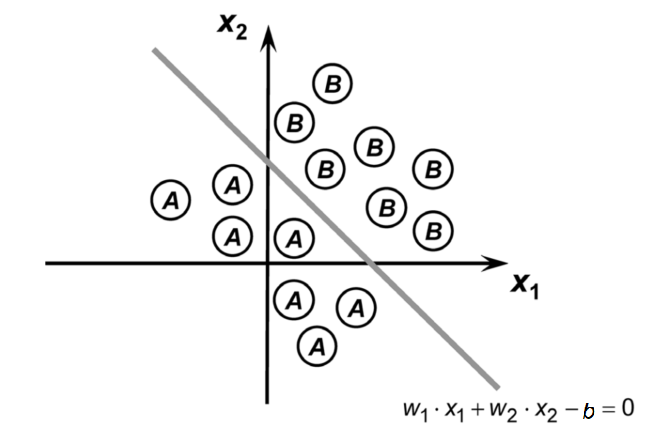
\includegraphics[width=.6\textwidth]{imagens/linearmente_separavel.png}}	

	{\scriptsize 	Fonte: \citeonline[p. 62]{silva_redes_2016}}
	\label{fig:linearmente_separavel}
\end{figure}

As redes neurais artificiais (\textbf{RNA}) se formam quando diversos neurônios se combinam. De forma resumida, ``uma rede neural artificial (RNA) pode ser vista como um grafo onde os nós são os neurônios e as ligações fazem a função das sinapses''. Isto está demonstrado na \autoref{fig:rna}.

\begin{figure}[h!]
	\centering
	\caption{Representação simplificada de uma RNA}	
	\fbox{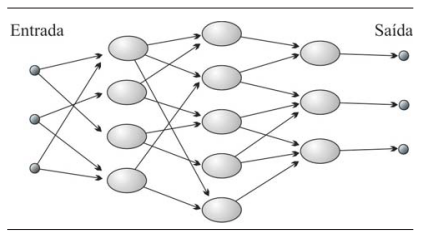
\includegraphics[width=.6\textwidth]{imagens/RNA.png}	}

	{\scriptsize 	Fonte: \citeonline[p.26]{ferneda_redes_2006}}
	\label{fig:rna}
\end{figure}

As  redes  neurais  artificiais  se  diferem  pelas  suas arquiteturas e pela forma como os pesos associados às conexões são ajustados durante o processo de aprendizado. A \textit{arquitetura} de uma rede neural restringe o tipo de problema no qual a rede poderá ser utilizada, e é definida pelo  número  de  camadas  (camada única  ou múltiplas camadas), pelo número de nós em cada camada, pelo tipo de conexão entre os nós (\textit{feedforward} ou \textit{feedback}) e por sua topologia \cite[p. 46-49]{haykin_redes_2001}.

O desenvolvimento de uma rede neural artificial consiste em determinar sua arquitetura, ou seja, os números de camadas e de neurônios em cada camada, bem como o ajuste dos pesos na fase conhecida como treinamento \cite{hagan_neural_1996} \cite{haykin_redes_2001}.

Uma das características mais importantes de uma rede neural artificial é a habilidade de aprender através de exemplos e fazer inferências sobre o que aprendeu, melhorando, assim, o seu desempenho. As RNA's utilizam um algoritmo de aprendizagem que serve, basicamente, para ajustar os pesos de suas conexões \cite{haykin_redes_2001} \cite{ferneda_redes_2006} \cite{lima_ia_2016} \cite{Norvig2013}. 

Aqui também há, cf. explicitado na seção \ref{aprendizagem_maquina}, duas formas básicas de aprendizado, o supervisionado e o não-supervisionado.

\subsection{Redes do tipo Perceptron de múltiplas camadas}
As arquiteturas do tipo perceptron de múltiplas camadas (MLP) são os modelos de redes neurais mais utilizados e conhecidos. Elas, basicamente, consistem de uma camada de entrada e uma ou mais camadas intermediárias (ou ocultas) além, claro da camada de saída (uma ou mais unidades sensoriais - neurônios) \cite{haykin_redes_2001}.

Os sinais de entrada são propagados camada a camada pela rede em uma direção, ou seja, da entrada para a saída (\textit{feedfoward}). Esta arquitetura retrata uma generalização do perceptron. Portanto, segundo \citeonline[p. 26]{silva_redes_2016}, 
\begin{citacao}
	As redes Perceptron de múltiplas camadas (PMC) são caracterizadas pela presença de pelo menos uma camada intermediária (escondida) de neurônios, situada entre a camada de entrada e a respectiva camada neural de saída.
\end{citacao}

Desta forma, elas possibilitam elevadas possibilidades de aplicações em muitas áreas do conhecimento, entre as principais: aproximação universal de funções, reconhecimento de padrões, identificação e controle de processos, previsões de séries temporais, otimização de sistemas entre muitos outros \cite{haykin_redes_2001}.

A \autoref{fig:pmc} ilustra uma rede do tipo perceptron de multicamadas. O treinamento deste tipo de rede é do tipo supervisionado e, geralmente, se utiliza um algoritmo muito popular chamado \textit{retropropagação} do erro (\textit{error backpropagation}). Este algoritmo é baseado numa regra de aprendizagem que “corrige” o erro durante o treinamento \cite{haykin_redes_2001}.

Substancialmente, o método de \textit{retropropagação} é constituído de duas etapas: uma fase de propagação do sinal no sentido tradicional (\textit{feedforward}) e uma de retropropagação do erro (\textit{backpropagation}) de todas as camadas e seus respectivos pesos. Na fase de ida, os vetores de dados e pesos são aplicados às unidades de entrada, e seu efeito se propaga pela rede, camada por camada \cite{hagan_neural_1996} \cite{haykin_redes_2001}.

Após isso, um conjunto de saídas é produzido como resposta da rede. Na retropropagação os pesos são ajustados de acordo com uma regra de correção de erro (normalmente uma função matemática como a \autoref{erro_absoluto}, a \autoref{erro_absoluto_medio}, a \autoref{erro_quadratico} ou \autoref{erro_quadratico_medio}, sendo esta última uma das mais utilizadas em muitas arquiteturas, na prática) \cite{haykin_redes_2001} \cite{hagan_neural_1996} \cite{yeung_neural_2004}.

A resposta da rede em um instante é subtraída da saída desejada (\textit{target}) para produzir um valor de erro. Este valor de erro é propagado da saída para a entrada, camada a camada, de onde vem o nome ``\textit{retropropagação} do erro''. Os pesos são, então, redefinidos de forma que a distância entre a resposta da rede e a resposta desejada seja reduzida (o erro seja minimizado). O processo é repetido diversas vezes até que uma tolerância global de erro seja assumida. Cada iteração é denominada época (\textit{epoch}) \cite{haykin_redes_2001} \cite{hagan_neural_1996} \cite{minsky_perceptrons:_1969}.

Uma arquitetura de um MLP (\textit{Multi-Layer Perceptron} - Perceptron Multicamadas), possui, portanto três propriedades distintas: a função de ativação, o número de camadas ocultas e forma das conexões (totalmente conectada ou não).

\begin{figure}[h!]
	\centering
	\caption{Rede Perceptron de multicamadas}
	\fbox{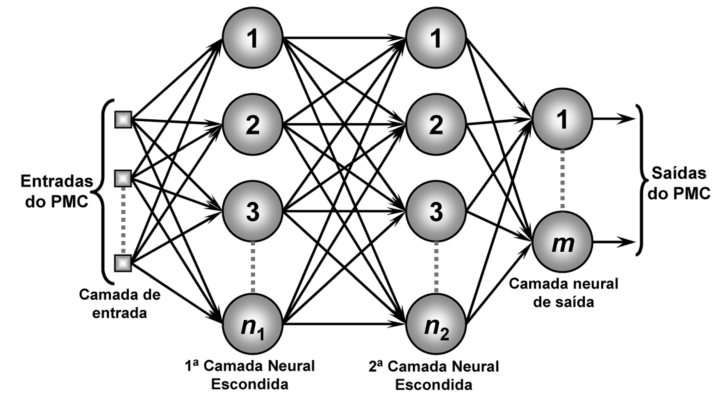
\includegraphics[width=.7\textwidth]{imagens/pmc.png}	}

	{\scriptsize 	Fonte: \citeonline[p. 92]{silva_redes_2016}}
	\label{fig:pmc}
\end{figure}

\subsection{Funções de ativação}\label{funcoes_ativacao}
Como visto na \autoref{perceptron}, o modelo perceptron, lida bem com problemas linearmente separáveis, mas tem problemas ao lidar com problemas  não-lineares \cite{haykin_redes_2001}. 

Para dar capacidade representativa às redes neurais artificiais, são essenciais as diferentes funções de ativação, pois só assim elas conseguirão lidar um componente de não-linearidade, como o são a maioria dos problemas práticos \cite{hagan_neural_1996}.

Ao se introduzir ativações não-lineares, a superfície de custo da rede neural deixa de ser convexa fazendo com que a otimização se torne mais difícil \cite{minsky_perceptrons:_1969} \cite{haykin_redes_2001}.

As principais funções de ativação, utilizadas na literatura ena prática, são, portanto:

\subsubsection{Função de ativação limiar}\label{ativacao:limiar}
Foi proposta na primeira definição de rede com neurônios artificiais \cite{rosenblatt_perceptron:_1958}. O modelo de neurônio usado por RosenBlatt foi o mesmo sugerido por \citeonline{mcculloch_logical_1943}. 

Neste modelo as saídas são binárias, ou seja, assumem, normalmente o valor 0 ou 1. A saída é 1 se o valor da entrada líquida for superior a um determinado valor chamado \textit{thereshold}. Na maioria das vezes, esse valor é zero.

Matematicamente:
\begin{equation}\label{eq:limiar}
	y_k = y = f_i(a_i(t)) = \left \{ 
	\begin{matrix} 1\textrm{,} & \mbox{\textrm{se }}a_i(t) >= 0 \\
	0\mbox{\textrm{,}} & \mbox{\textrm{se }}a_i(t) < 0 \end{matrix} 
	\right.
\end{equation}

A \autoref{fig:binary_step} mostra o `funcionamento' da função de ativação limiar. Eventualmente podem ser utilizados os valores -1 e 1. Uma rede de camada simples que utiliza este tipo de ativação é o perceptron simples.

\begin{figure}[h!]
	\centering
	\caption{Função de ativação Limiar}
	\fbox{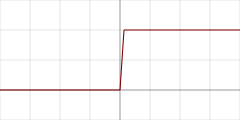
\includegraphics[width=.5\textwidth]{imagens/binary_step.png}	}

	{\scriptsize 	Fonte: Adaptado de \citeonline{haykin_redes_2001}}
	\label{fig:binary_step}
\end{figure}

\subsubsection{Função de ativação linear}\label{ativacao:linear}
A saída do neurônio, neste caso, é representada por uma função linear da forma descrita na \autoref{fig:ativacao_linear}. Redes que usam este tipo de função de ativação apresentam apenas uma camada de entrada e uma de saída. Possuem, portanto, uma série de representações quanto ao que são capazes de representar \cite{lima_ia_2016}.

\begin{figure}[h!]
	\centering
	\caption{Função de ativação Linear}
	\fbox{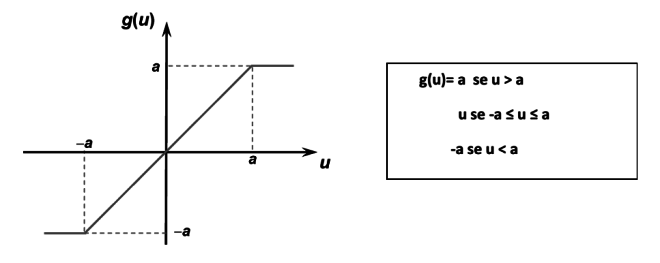
\includegraphics[width=.5\textwidth]{imagens/ativacao_linear.png}	}

	{\scriptsize Fonte: Adaptado de \citeonline{haykin_redes_2001}}
	\label{fig:ativacao_linear}
\end{figure}

\subsubsection{Funções de ativação semilineares}\label{ativacao_semilinear}
As funções de ativação mais usadas deste tipo são a função logística e a tangente hiperbólica. Elas são populares por conta de suas derivadas (que são necessárias nas etapas de treinamento, particularmente no \textit{Gradiente Descent} --- descida do gradiente) poderem ser expressas a partir das próprias funções.

Estas funções, tanto a logística (ou \textit{sigmoide}) e a tangente hiperbólica, respectivamente, podem ser expressas pelas equações \ref{eq:sigmoide_tanh} abaixo, onde $a$ representa a entrada líquida da unidade \cite{haykin_redes_2001} \cite{lima_ia_2016}.

\begin{equation}\label{eq:sigmoide_tanh}
	f(a) = \frac{1}{1+ e^{(-2 \beta a)}} \qquad g(a) = tanh(\beta a)
\end{equation}

E as respectivas derivadas das funções \ref{eq:sigmoide_tanh} acima são dadas por:

\begin{equation}\label{derivadas_sigmoide_tanh}
	f'(a) = 2 \beta f(1-f) \qquad g'(a) = \beta (1-g^2)
\end{equation}

A \autoref{fig:ativacao_sigmoide} mostra o comportamento da função sigmoide e a \autoref{fig:tanh} demonstra o da função tangente hiperbólica.

\begin{figure}[h!]
	\centering
	\caption{Função de ativação Logística (sigmoide)}
	\fbox{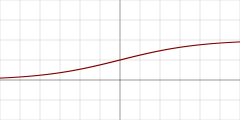
\includegraphics[width=.5\textwidth]{imagens/logistic.png}}
	
	{\scriptsize 	Fonte: Adaptado de \citeonline{haykin_redes_2001}}
	\label{fig:ativacao_sigmoide}
\end{figure}

\begin{figure}[h!]
	\centering
	\caption{Função de ativação Tangente Hiperbólica}
	\fbox{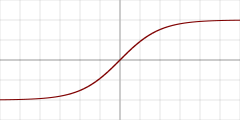
\includegraphics[width=.5\textwidth]{imagens/tanh.png}	}
	
	{\scriptsize 	Fonte: Adaptado de \citeonline{haykin_redes_2001}}
	\label{fig:tanh}
\end{figure}

\subsubsection{Função de ativação ReLu}
A função ReLU é a unidade linear retificada. É definida como, \citeonline{deep_learning_book_2019}:
\begin{equation}\label{relu}
	ReLU(x) = max(0,x)
\end{equation}
Sua derivada é dada por:
\begin{equation}\label{derivada_relu}
	ReLU'(x) = \left \{ \begin{matrix} 1, & \mbox{se }x > 0 \\ 
	0, & \mbox{\textrm{caso contrário}} \end{matrix} \right.
\end{equation}
Conforme, \citeonline{deep_learning_book_2019},
\begin{citacao}
	 ReLU é a função de ativação mais amplamente utilizada ao projetar redes neurais atualmente. Primeiramente, a função ReLU é não linear, o que significa que podemos facilmente copiar os erros para trás e ter várias camadas de neurônios ativados pela função ReLU.
\end{citacao}
Ainda, de acordo com \citeonline{deep_learning_book_2019}: 
\begin{citacao}
	A principal vantagem de usar a função ReLU sobre outras funções de ativação é que ela não ativa todos os neurônios ao mesmo tempo. [...] Se [...] a entrada for negativa, ela será convertida em zero e o neurônio não será ativado. Isso significa que, ao mesmo tempo, apenas alguns neurônios são ativados, tornando a rede esparsa e eficiente e fácil para a computação.
\end{citacao}

A \autoref{fig:relu} demonstra o comportamento da função de ativação ReLu em função da entrada

\begin{figure}[h!]
	\centering
	\caption{Função de ativação ReLu - unidade linear retificada}
	\fbox{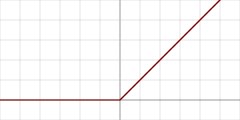
\includegraphics[width=.5\textwidth]{imagens/relu.png}	}
	
	{\scriptsize 	Fonte: Adaptado de \citeonline{haykin_redes_2001}}
	\label{fig:relu}
\end{figure}

Redes com a função ReLU são mais fáceis de otimizar porque a função é parecida com a função identidade. A única diferença é que a ReLU produz zero em metade de seu domínio \cite{hagan_neural_1996}.

\subsection{Otimização}\label{otimização}
Redes Neurais tem uma etapa iterativa em que os pesos são ajustados e se pode realizar otimizações para melhorar o erro e incrementar o modelo \cite{haykin_redes_2001}.

Normalmente, o fluxo de treinamento se resume nos seguintes passos iterativos:
\begin{enumerate}\label{fluxo_treinamento}
	\item Operar a entrada na rede
	\item Cálculo da função de perda (\textit{loss function}) ou outra função de cálculo de erro
	\item Cálculo do gradiente
	\item Atualização dos pesos
	\item Volta para o passo 1
\end{enumerate}

Este processo é repetido até que um hiperparâmetro de tolerância seja alcançado para o cálculo dos erros mediante a \textit{loss function} ou outra função de cálculo do erro.

O cálculo do gradiente descrito anteriormente diz respeito, cf. \citeonline{deep_learning_book_2019} a um dos mais usados algoritmos para otimizar a tarefa de aprendizagem dos pesos de uma rede neural.

De acordo com \citeonline{deep_learning_book_2019}: 
\begin{citacao}
	A Descida do Gradiente é uma ferramenta padrão para otimizar funções complexas iterativamente dentro de um programa de computador. Seu objetivo é: dada alguma função arbitrária, encontrar um mínimo. Para alguns pequenos subconjuntos de funções – aqueles que são convexos – há apenas um único \textit{minimum} que também acontece de ser global. Para as funções mais realistas, pode haver muitos mínimos, então a maioria dos mínimos são locais.[... É preciso] que a otimização encontre o “melhor” \textit{minimum} e não fique preso em mínimos sub-otimistas (um problema comum durante o treinamento do algoritmo).
\end{citacao}

O algoritmo consiste basicamente de subtrair o valor do gradiente $\nabla f$ dos pesos $w$ da rede, assim:
\begin{equation}\label{gradiente}
	w_i = w_i - \alpha \times \nabla f_i
\end{equation}
Sendo $\alpha$ o multiplicador que nos permite controlar o tamanho do passo de otimização.  $\nabla f$ é a derivada da função de ativação no ponto específico. $\alpha$ é um hiperparâmetro conhecido como taxa de aprendizado e repreenta a \textit{velocidade} em que a rede neural ``aprende'' os melhores pesos para o problema específico \cite{haykin_redes_2001}.

Uma iteração consiste em um passo de otimização como o descrito em \ref{fluxo_treinamento} e corresponde a uma ligação sináptica de \textit{forward} na rede e uma de \textit{backpropagation}. Isto constitui uma \textbf{\underline{época}}. Normalmente, muitas épocas são necessárias, visto que o aprendizado em uma rede neural é, geralmente, lento para que a otimização evite os mínimos locais.

Na próxima seção, conceitos sobre SVM (Support Vector Machines) serão descritos e explorados. Este será o segundo algoritmo utilizado neste trabalho para sustentar a hipótese, juntamente com as RNA's.

\section{SVM - Support Vector Machines}\label{SVM}
Segundo \citeonline{cortes_svm_1995}, o algoritmo SVM (\textit{Support Vector Machines}) é um dos mais efetivos para a tarefa de classificação.

Conforme \citeonline{goldschmidt2005},
\begin{citacao}
	No algoritmo SVM, o conjunto de dados de entrada é utilizado para construir uma \textit{função de decisão} $f(x)$, tal que:	
		\begin{equation}
			\begin{matrix}
				Se & f(x_i) \ge 0, &\textrm{então}&  y_i = 1   \\
				Se & f(x_i) < 0,   &\textrm{então}&  y_i = -1   
			\end{matrix}
		\end{equation}

	O algoritmo SVM constrói os denominados classificadores lineares, que separam o conjunto de dados por meio de um \textit{hiperplano} que é a generalização do conceito de \textit{plano} para dimensões maiores que três.	
\end{citacao}

Assim, SVM, cf. \citeonline[p. 45]{aprenda_mineracao_fernando_amaral16} ``são um algoritmo de classificação que maximizam as margens entre instâncias mais próximas, dessa forma, é criado um vetor otimizado que é então utilizado para classificar novas instâncias''.

Conforme se vê na \autoref{fig:svm}, os dois vetores \textit{não pontilhados} são as margens otimizadas. As instâncias por onde as margens otimizadas passam são os vetores de suporte. O vetor pontilhado é a referência para classificar novas instâncias. Assim, a nova instância, na \autoref{fig:svm} é classificada como triângulo.

\begin{figure}[h!]
	\centering
	\caption{Vetores de Suporte}
	\fbox{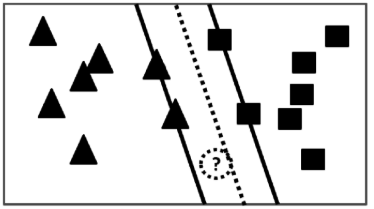
\includegraphics[width=.6\textwidth]{imagens/vetores_de_suporte.png}	}
	
	\label{fig:svm}
	{\scriptsize 	Fonte: \citeonline[p. 45]{aprenda_mineracao_fernando_amaral16}}
\end{figure}

Seguindo o estudo de \citeonline{mukkamala_intrusion_2002} há duas razões principais que levaram os autores do artigo citado de usarem SVMs para detecção de intrusão: o primeiro é a velocidade já que a performance é prioritariamente uma das características mais importantes para sistemas de detecção de intrusos. 

A segunda razão é a escalabilidade, pois, cf. os autores, SVMs são relativamente indiferentes ao número de \textit{data points} e a complexidade da classificação não depende da dimensionalidade do espaço de características. Dependendo da aplicação, ainda conforme os autores, uma vez que os dados estão classificados em duas classes, um algoritmo de otimização adequado pode ser usado, se necessário,  para identificação de mais características.

Embora os classificadores lineares SVM sejam eficientes e funcionem surpreendentemente bem em muitos casos, alguns conjuntos de dados não são linearmente separáveis. Adicionar mais características (dimensões), como as polinomiais é uma abordagem válida para lidar com os conjuntos de dados não lineares; em alguns casos, isso pode resultar em um conjunto de dados linearmente separável. \cite[p. 153]{geron_maos_2020}

Na \autoref{fig:svm-nao-linear} observa-se que na plotagem à esquerda um conjunto de dados simples com apenas uma característica $ x_1$. Esse conjunto não é linearmente separável (como a imagem mostra), mas se for adicionada uma segunda característica $ x_2 = (x_1)^2 $, o conjunto de dados resultante será linearmente separável.

\begin{figure}[h!]
	\centering
	\caption{Adição de características para tornar um conjunto linearmente separável}
	\fbox{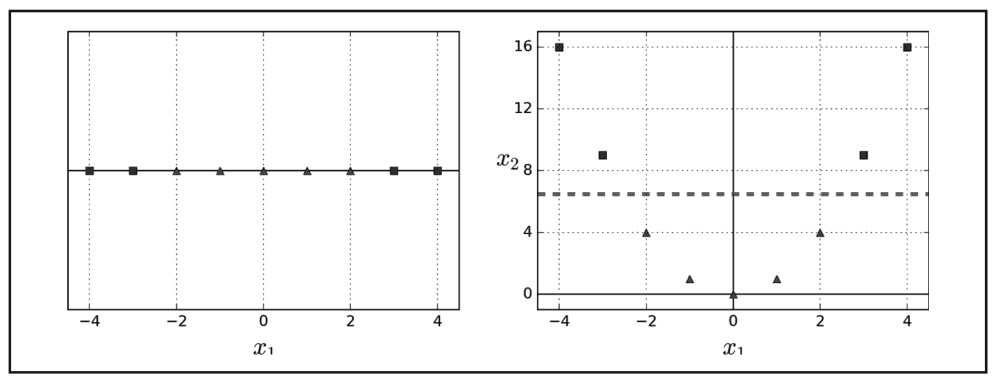
\includegraphics[width=.8\textwidth]{imagens/svm-adicionando-caracteristicas.png}	}
	
	\label{fig:svm-nao-linear}
	{\scriptsize 	Fonte: \citeonline[p. 153]{geron_maos_2020}}
\end{figure}

Isto pode ser visualizado na \autoref{fig:svm-polinomial} que também mostra a adição de características para tornar um problema linearmente separável.
\begin{figure}[h!]
	\centering
	\caption{Classificador Linear SVM com o uso de características polinomiais}
	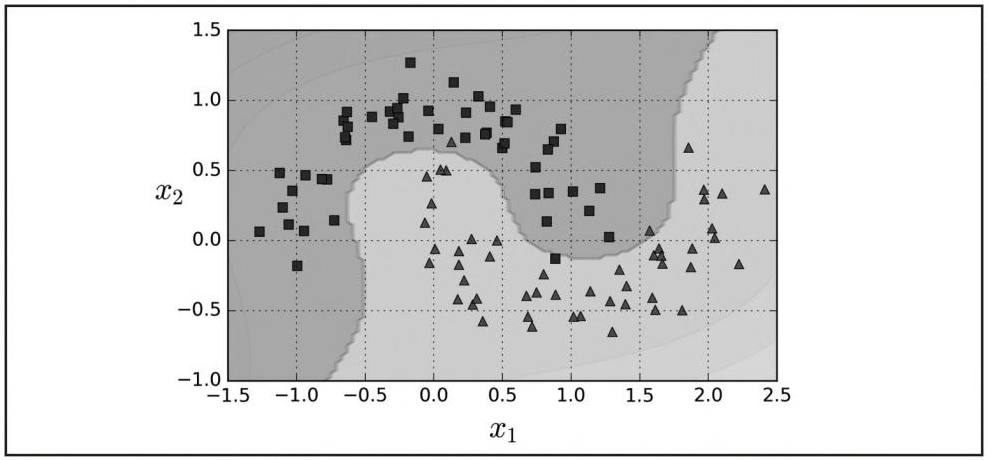
\includegraphics[width=.8\textwidth]{imagens/svm-polinomial.png}
		
	\label{fig:svm-polinomial}
	{\scriptsize 	Fonte: \citeonline[p. 154]{geron_maos_2020}}
\end{figure}

Neste trabalho, também foi usado, com eficácia que suportasse a hipótese (cf. se vê no \autoref{resultados}) o algoritmo SVM.

Ainda vou escrever aqui nesta seção sobre SVM acerca de: kernel, RBF Gaussiana, complexidade, função de decisão, Hinge Loss, otimização por meio de multiplicadores de Lagrange, modelo de estimação de função e otimização matemática.

\section{Trabalhos Relacionados}\label{trabalhos_relacionados}
Esta seção expõe alguns dos principais trabalhos encontrados na literatura que estão, de alguma forma, relacionados a esta dissertação. Foram estudadas e analisados trabalhos acerca das políticas de segurança da informação, abordando a detecção de conflitos em diversos contextos como identificação e resolução de conflitos aéreos, rodoviários e de \textit{normas} além de trabalhos sobre mineração de dados e técnicas de aprendizagem de máquina tanto em conjunturas distintas como regressão e classificação quanto para localização e solução de conflitos, no caso específico das políticas computacionais, principalmente sendo usadas em registros de patentes americanas fechadas --- o que, de certa forma, evidencia o quanto este tema está na vanguarda.

Todos os trabalhos descritos foram base para o estudo, amadurecimento bibliográfico e aprofundamento teórico sobre o problema e as soluções propostas neste trabalho, principalmente aqueles relacionados a intrusões, detecção de conflitos aéreos e as soluções baseadas em aprendizado de máquina, usando classificadores utilizados neste trabalho, como k-NN, Naïve Bayes, Random Forest, redes neurais e máquinas de vetores de suporte (SVM) pois serviram de inspiração e ofereceram estímulo para que as técnicas pudessem ser extrapoladas para o uso na detecção de conflitos em políticas, tema desta de dissertação. 

Como forma de organização, os trabalhos serão divididos em 4 seções:\begin{itemize}
	\item Verificação Detecção de conflitos;
	\item Mineração de Políticas;
	\item Resolução de outros tipos conflitos e 
	\item mineração de dados e aprendizagem de máquina em geral.
\end{itemize}

\subsection{Verificação e Detecção de conflitos}\label{sec:deteccao-conflitos}
\subsubsection{\citeonline{sarkis2017} }
Estes são os trabalhos-base no estudo da detecção de conflitos, da determinação do modelo das políticas utilizadas e analisadas além de serem a fonte de algumas das principais definições empregadas nesta dissertação. \citeonline{sarkis2017} propõe uma abordagem para detectar conflitos indiretos entre políticas. Assim, as contribuições deste trabalho incluem: a definição da política utilizada; o conjunto de relacionamentos que podem ocorrer entre os atributos que compõem uma política (organização, sujeitos, papéis, objetos, visões, ação e atividades); o conjunto de regras de propagação e de regras de conflitos (utilizados nos conflitos indiretos). Uma ferramenta foi desenvolvida, o  ``Conflict Detector'' que recebe como entrada um conjunto de políticas de controle de acesso, um conjunto de relacionamentos entre os atributos destas políticas e fornece como saída, no caso da existência de conflitos, a identificação do conflito e as políticas conflitantes.

\subsubsection{\citeonline{vijayalakshmi_priority-based_2020} }
Este artigo analisa e detecta as anomalias importantes nas políticas de controle de acesso baseadas em atributos---ABAC. Apresenta uma abordagem que usa o nível de prioridade para evitar o conflito nas políticas. Esta abordagem agrupa as regras das políticas ABAC com base no nível de prioridade e semelhança com a técnica de agrupamento, e detecta as anomalias em cada cluster em vez de todas as regras.

\subsubsection{\citeonline{zheng_research_2019} }
Aborda o controle de acesso baseado em atributos (ABAC) nos contextos da computação em nuvem e Internet das coisas. Cita que os conflitos entre as de políticas ocorrem com frequência devido à sua grande escala e expressão complexa. O trabalho propõe, então, um novo método para detectar conflitos entre regras ABAC com o auxílio da conversão de regras em um conjunto de sequências binárias. Em seguida, a detecção de conflito é alcançada através da operação bit a bit AND da sequência binária, o que melhora a eficiência da detecção.

\subsubsection{\citeonline{yahiaoui_deconflicting_2018} }
Também aborda o controle de acesso baseado em atributos (ABAC) afirmando que este pode trazer grandes benefícios no contexto de compartilhamento e proteção de dados confidenciais. Declara também que esses sistemas são complexos de analisar e geralmente sofrem de anomalias e conflitos entre as políticas de segurança. Neste artigo, os autores lidam com o problema de várias políticas fornecerem respostas conflitantes (permitir / negar) para uma mesma solicitação de acesso e é proposta uma estrutura que pode apoiar os administradores de segurança com ferramentas para analisar, detectar e resolver continuamente quaisquer possíveis conflitos nos sistemas ABAC.

\subsubsection{\citeonline{eduardo2017} } 
Este trabalho estuda a verificação de conflitos entre múltiplas normas em sistemas multiagentes (SMA). As normas, nesta tese, são semelhantes às políticas, inclusive em suas definições, mas restritas a um contexto de agentes autônomos. Para a resolução de conflitos, o autor usa uma estratégia de aplicação de filtros para suavizar o custo computacional e utiliza transformação deôntica para análise de diversas normas ao mesmo tempo. %Cf. discutido na \autoref{justificativa}, estas estratégias levam a um problema NP-Completo.

\subsubsection{\citeonline{sun_privacy_2011} }
Este artigo propõe uma estrutura para políticas e mecanismos de controle de acesso que preservam a privacidade e descreve algoritmos para problemas conflitantes de políticas de acesso. O mecanismo reforça a política de acesso aos dados que contêm informações de identificação pessoal. O principal componente da estrutura é o \textit{propósito} envolvido nos modelos de controle de acesso (PAC) que fornecem suporte para expressar políticas complexas relacionadas à privacidade, levando em consideração recursos como objetivos, condições e obrigações. Os autores comentam que podem surgir problemas de conflito de políticas quando novas políticas de acesso são geradas e podem entrar em conflito com as políticas existentes. A estrutura da política de controle de acesso, incluindo condições e obrigações, é estudada. Com base na política de acesso, os modelos de autorização e as operações de política são analisados. E, também os conflitos entre as políticas.

\subsubsection{\citeonline{hwang_acpt_2010}}
Como \citeonline{sarkis2017}, os autores também desenvolvem uma ferramenta para resolver o problema da detecção de conflitos, chamada  ACPT (Teste de Política de Controle de Acesso), que ajuda a modelar e implementar políticas corretamente durante a modelagem, implementação e verificação de políticas.

\subsubsection{\citeonline{shu_detecting_2009}}
Este artigo propõe um método otimizado para detectar os conflitos entre regras estatisticamente conflitantes em uma política ABAC. O método inclui duas técnicas de otimização: redução de regras e busca binária. As políticas ABAC são fartamente explicadas e exploradas neste trabalho.

\subsubsection{\citeonline{he_Qingfeng_2009} }
Os autores afirmam que a especificação de políticas de controle de acesso não é uma parte explícita do processo de desenvolvimento de software e geralmente é isolada das atividades de análise de requisitos,deixando,assim, os sistemas vulneráveis ​​a violações de segurança porque as políticas são especificadas sem garantir a conformidade com os requisitos do sistema. No artigo, então, é apresentado o método ReCAPS (Análise de Controle de Acesso com Base em Requisitos e Especificação de Política) para derivar e especificar políticas de controle de acesso e discutir esforços de validação. O método integra a especificação de política no processo de desenvolvimento de software e garante a consistência entre os artefatos de software além de fornecer orientação prescritiva sobre como especificar políticas de controle de acesso.

\subsubsection{\citeonline{ferraiolo_policy_2011}}
Neste artigo, os autores poopõem uma estrutura de controle de acesso, conhecida como Policy Machine (PM), que muda a maneira como a política é expressa e aplicada. trabalha com polítics de Controle de Acesso Discricionário e Controle de Acesso Baseado em Funções.

\subsubsection{\citeonline{mohan_detection_2012}}
Neste artigo os autores propõem e avaliam duas estratégias, uma para detectar inconsistências de políticas para evitar possíveis ataques de inferência e outra para detectar conflitos de políticas dentro do contexto de dados armazenados em bancos de dados biomédicos derivados de ontologias biomédicas.

\subsection{Mineração de políticas}\label{sec:mineracao-politicas}
\subsubsection{ \citeonline{bui_greedy_2019} }
O contexto do estudo é o controle de acesso baseado em relacionamento (ReBAC) que, segundo os autores, fornece um alto nível de expressividade e flexibilidade que promove a segurança e o compartilhamento de informações. O ReBAC é como uma extensão orientada a objetos do controle de acesso baseado em atributos (ABAC) em que os relacionamentos são expressos usando campos que se referem a outros objetos e as expressões de caminho são usadas para seguir cadeias de relacionamentos entre objetos. Este artigo apresenta dois algoritmos para mineração de políticas ReBAC: um algoritmo guloso guiado por heurísticas e um algoritmo evolutivo baseado em gramática. Os autores afirmam que os algoritmos de mineração de políticas ReBAC têm potencial para reduzir significativamente o custo de migração de sistemas de controle de acesso legados para ReBAC, automatizando parcialmente o desenvolvimento de uma política ReBAC a partir de uma política de controle de acesso existente.

\subsubsection{\citeonline{chakraborty_feasibility_2019}}
O artigo aborda a tecnologia de controle de acesso baseado em atributo (ABAC) focando no problema de converter políticas de sistemas de controle de acesso já implantados para ABAC. Diversas variações desse problema geral podem ser definidas, em particular, o problema de mineração de política ABAC. Neste artigo, os autores formalizam o problema de existência do ABAC RuleSet neste contexto e desenvolvem um algoritmo e uma análise de complexidade para sua solução. Introduzimos ainda a noção de Correção de inviabilidade do conjunto de regras ABAC junto com um algoritmo para a solução.

\subsubsection{\citeonline{kalaskar_fp-growth_2018} }
Neste artigo, os autores propõem uma técnica conhecida como algoritmo de FP-Growth para minerar regras de associação no contexto de uso desse algoritmo ter a capacidade de reduzir o custo de migração para ABAC. O artigo mostra o algoritmo na mineração de políticas ABAC. 

\subsubsection{\citeonline{xu_mining_2013} }
O controle de acesso baseado em funções (RBAC) é amplamente usado, mas tem limitações notáveis, o que leva a uma mudança para o controle de acesso baseado em atributos (ABAC). No entanto, o custo de desenvolver uma política ABAC pode ser um obstáculo significativo para a migração do RBAC para o ABAC. Este artigo apresenta a primeira definição formal do problema de mineração de políticas ABAC a partir de políticas RBAC e dados dos atributos, e o primeiro algoritmo projetado especificamente para extrair uma política ABAC de uma política RBAC e dados dos atributos.

\subsubsection{\citeonline{hachana_mining_2015} }
Neste artigo, os autores fazem uma abordagem de mineração de políticas por meio de um processamento adicional para uma mineração de políticas de controle de acesso à rede. Desenvolvem o problema de integração de políticas Net-RBAC resultantes da mineração de políticas em vários firewalls. Além disso, mostram como verificar as propriedades de segurança relacionadas à consistência da implantação nos firewalls. Usam, portanto, a mineração de dados em políticas de controle de acesso em um contexto de regras de um firewall (na realidade, de vários firewalls).

\subsubsection{\citeonline{martin_inferring_2006}}
Segundo os autores, para aliviar a carga de implementação e manutenção de aspectos de controle de acesso em um sistema, uma tendência crescente entre os desenvolvedores é escrever políticas de controle de acesso em uma linguagem de especificação, como XACML e integrar as políticas com aplicativos através do uso de um ponto de decisão de política ( PDP). Para garantir que as políticas especificadas reflitam as esperadas, pesquisas desenvolveram ferramentas de verificação de políticas; no entanto, seus aplicativos na prática ainda são limitados, sendo restringidos pelo conjunto limitado de recursos de linguagem de política suportados e a indisponibilidade de propriedades de política. Este artigo apresenta uma abordagem de mineração de dados para o problema de verificar se as políticas de controle de acesso expressas refletem os verdadeiros desejos do autor da política. Foi desenvolvida uma ferramenta para investigar essa abordagem gerando solicitações automaticamente, avaliando essas solicitações para obter respostas e aplicando o aprendizado de máquina aos pares de solicitação-resposta para inferir propriedades de política. Essas propriedades inferidas facilitam a inspeção do comportamento da política. Os resultados mostram que algoritmos de aprendizado de máquina podem fornecer informações valiosas sobre as propriedades básicas da política e ajudar a identificar solicitações específicas de exposição a bugs.

\subsection{Detecção e Resolução de outros tipos conflitos}\label{trab:rel-conflitos}
\subsubsection{\citeonline{lupu_conflicts_1999}}
Os autores deste trabalho discorrem sobre conflitos no gerenciamento de sistemas distribuídos com base em políticas de controle de acesso. O artigo analisa os conflitos de políticas, concentrando-se nos problemas de detecção e resolução dos mesmos. Discute-se, no artigo, os vários relacionamentos de precedência que podem ser estabelecidos entre as políticas e é apresentado uma ferramenta de análise de conflitos que faz parte de uma estrutura de gerenciamento baseada em funções, porém, sem usar mineração de dados ou aprendizagem de máquina.

%\subsubsection{\cite{koch_conflict_2002}}
%O artigo estudou,  usando como base grafos, a detecção e resolução de conflitos nas especificações das políticas de controle de acesso. Os autores usam propriedades formais de transformações de grafos para detectar sistematicamente inconsistências entre restrições, entre regras e entre uma regra e uma restrição em políticas de controle de acesso e estabelecer as bases para suas resoluções,  porém, também não usando mineração de dados ou aprendizagem de máquina.

\subsubsection{\citeonline{chen_flight_2011} e \citeonline{christodoulou_collision_2008}}
O artigo de \citeonline{chen_flight_2011} trabalha com a identificação e a resolução de conflitos de voo com base em \textit{redes neurais}. No artigo, o autor considera os problemas de detecção e resolução de conflitos no gerenciamento de tráfego aéreo (ATM - \textit{Air Traffic Management}) sob a perspectiva da geometria computacional e fornece algoritmos para resolver esses problemas além de propor um método que pode rotear várias aeronaves, sem conflitos, através do espaço aéreo, usando um esquema de roteamento priorizado no espaço-tempo através do uso de conjunto de soluções ótimas por meio de uma rede neural. Já o trabalho de \citeonline{christodoulou_collision_2008} aborda a detecção de conflitos sobre a ótica da prevenção de colisões no voo livre de aeronaves comerciais usando redes neurais com exemplos preparados por meio de programação não linear. 

%\subsubsection{\cite{neri_conflict_2012}}
%Os autores abordaram a detecção de conflitos em políticas de segurança usando as tecnologias da Web Semântica. É mostrado, no artigo, como as ferramentas fornecidas pelas tecnologias de gerenciamento de Web Semântica e Ontologia oferecem uma base adequada para a realização de técnicas capazes de suportar a análise de conflitos nas políticas de segurança. Com base no uso dessas técnicas, é proposto no artigo, uma solução para duas variantes diferentes de análise de conflitos: (a) incompatibilidade de políticas e (b) satisfação de separação de tarefas. 



\subsection{Mineração de dados e aprendizagem de máquina}\label{trab-rel:MD e AM}
\subsubsection{\citeonline{guerrero-higueras_detection_2018}}
\citeonline{guerrero-higueras_detection_2018} aborda um método para construir modelos de \textit{aprendizagem de máquina} com o objetivo de detectar ataques cibernéticos em RTLSs (\textit{Real Time Location Systems} - sistemas de localização em tempo real) em um ambiente de cibersegurança para sistemas robóticos usando técnicas de \textit{Machine Learning}.  O artigo mostra que os ciberataques nos sistemas de localização em tempo real para sistemas robóticos podem ser detectados por um sistema criado usando o aprendizado supervisionado. Além disso, mostra que alguns tipos de ciberataques em sistemas de localização em tempo real, especificamente negação de serviço e falsificação(\textit{DoS} e \textit{Spoofing}), podem ser detectados por um sistema construído usando técnicas de aprendizado de máquina. Oito classificadores e algoritmos preditores conhecidos foram avaliados neste artigo e a análise de validação cruzada mostrou que os classificadores MLP (\textit{Multi Layer Perceptron}) funcionam melhor que os outros obtendo maior acurácia e menor erro, sendo também o modelo com menor \textit{overfitting} e maior \textit{sensibilidade}\footnote{Sensibilidade é a proporção de verdadeiros positivos: a capacidade do sistema em predizer corretamente a condição para casos que realmente a têm - É também conhecida como \textit{\textbf{Recall}}.}. Este artigo inspirou a hipótese desta proposta de dissertação.

\subsubsection{\citeonline{bui_efficient_2019}}
\citeonline{bui_efficient_2019} versa acerca de mineração de dados em políticas de controle de acesso, especificamente do modelo ReBAC (\textit{Relationship-Based Access Control} - controle de acesso baseado em \textit{relacionamento}), mas não foca na detecção de conflitos entre as políticas, e sim, na propagação de seus relacionamentos na criação de novas políticas. No artigo, os algoritmos de mineração de política do ReBAC propostos puderam reduzir significativamente o custo da migração dos sistemas de controle de acesso legados para o ReBAC, automatizando parcialmente o desenvolvimento de uma nova política do ReBAC.

\subsubsection{\citeonline{obaidat_multilayer_1994} e \citeonline{mukkamala_intrusion_2002}}
\citeonline{obaidat_multilayer_1994} aborda um sistema de rede neural multicamadas para segurança de acesso a computadores com o objetivo de identificar usuários do mesmo. Os vetores de entrada foram compostos pelos intervalos de tempo entre pressionamentos de teclas sucessivos criados pelos usuários ao digitar uma sequência conhecida de caracteres. Usando aprendizado supervisionado, cada vetor de entrada foi classificado em uma das várias classes, identificando assim o usuário que digitou a sequência de caracteres. Neste artigo, uma precisão máxima de classificação de 97,5\% foi alcançada usando um classificador de padrões baseado em rede neural multicamadas \textit{feedforward} treinada usando \textit{backpropagation}, o algoritmo de retropropagação. Essa abordagem visa melhorar a segurança do acesso ao computador. Este artigo trouxe contribuições para esta proposta de dissertação na maneira de construir a arquitetura da rede neural e também no ajuste dos \textit{hiperparâmetros}. Na mesma linha, o artigo de \citeonline{mukkamala_intrusion_2002} estuda a detecção de invasões usando redes neurais e máquinas de vetores de suporte e a ideia central é descobrir padrões úteis ou características que descrevam o comportamento intrusivo de um usuário em um sistema e os autores usam este conjunto de características para construir classificadores que puderam reconhecer anomalias e intrusões conhecidas em tempo real. É usado um conjunto de dados de referência de uma competição de KDD (\textit{Knowledge Discovery in Databases} --- Descoberta de Conhecimento em Bases de Dados) projetada pela DARPA (Defense Advanced Research Projects Agency), e é demonstrado que classificadores eficientes e precisos podem ser construídos para detectar invasões. Ao final é comparado o desempenho de redes neurais e máquinas de vetores de suporte para a detecção de intrusões. Nesta proposta de dissertação, baseando-se neste artigo de \citeonline{mukkamala_intrusion_2002} também serão avaliados os desempenhos de redes neurais e máquinas de vetores de suporte, mas para detecção de conflitos em políticas.

\subsubsection{\citeonline{jin_development_2002} e \citeonline{debar_neural_1992}}
O trabalho de \citeonline{jin_development_2002} aborda o desenvolvimento e uso de uma rede neural probabilística construtiva (\textbf{CPNN} - \textit{Constructive Probabilistic Neural Network}) na detecção de incidentes em rodovias, incluindo a construção e adaptação dos modelos. Esta CPNN foi estruturada com base no modelo Gaussiano de mistura e treinada por um algoritmo de ajuste dinâmico de decaimento (para correção dos erros). Os incidentes em rodovias, como colisões de veículos, podem ser extrapolados para um modelo de conflito entre agentes de um sistema. O modelo foi treinado e avaliado sobre um banco de dados de incidentes simulados em Singapura e adaptado para a rodovia I-880 na Califórnia sendo então investigada em ambientes on-line e off-line. Este artigo citado compara o desempenho do modelo CPNN e um modelo de rede neural probabilística básica (BPNN - Basic Probabilistic Neural Network).Já o artigo de \citeonline{debar_neural_1992} estuda um componente de rede neural para um sistema de detecção de intrusão. O modelo \textit{aprende} os hábitos que um usuário tem enquanto trabalha com o computador e emite avisos quando o comportamento atual não é consistente com os padrões \textit{aprendidos} anteriormente. O modelo de de rede neural  é usado para modelar o comportamento do usuário como uma característica componente para o sistema de detecção de intrusão.
%\subsubsection{\cite{ahuja_54_nodate}}
%Importante citar a patente assinada pelos inventores \citeonline{ahuja_54_nodate}, ``Sistema e método para mineração de dados e gerenciamento de políticas de segurança'', tendo a  McAfee como cessionária, que propõe um método para mineração de dados automatizada e criação de políticas de segurança em redes e sistemas.

\subsection{Relacionamento dos trabalhos com a dissertação}
Na detecção de conflitos em políticas, usam-se, comumente, abordagens como as de \citeonline{sarkis2017} e \citeonline{mohan_detection_2012} --- estritamente analíticas e formais, baseadas em análise de ontologias entre os atributos que compõem uma política e os relacionamentos e regras de propagação destas políticas ou mesmo estratégias como as de \citeonline{wang_conflicts_2010} e \citeonline{ferraiolo_policy_2011} que usam uma arquitetura que pode ser empregada como uma máquina de proteção de propósito geral usando métodos matemáticos formais para atingir seus objetivos. Dentro do conjunto de modelos formais, envolvendo relacionamentos, na detecção de conflitos, há também o trabalho de \citeonline{sun_privacy_2011}, que usa o ``propósito envolvido nos modelos de controle de acesso'' para atingir seu fim. \textit{Estes, fatalmente, analisam as políticas em pares ou em grupos sem filtros de agrupamentos}.

Existem os métodos baseados em requisitos como os propostos por \citeonline{he_Qingfeng_2009} que integram a especificação de política no processo de desenvolvimento de software, garantindo, assim, a consistência entre os artefatos de software e fornecendo orientação prescritiva sobre como especificar ACPs (\textit{Access Control Policies)} --- políticas de controle de acesso, mas que\textit{ tem o inconveniente de ocorrer durante o desenvolvimento e a fase de análise do sistema e não em tempo de execução do mesmo}.

Há, na literatura especializada são encontrados procedimentos como os descritos em \citeonline{eduardo2017} que utilizam lógica deôntica\footnote{A lógica \textit{deôntica} é um tipo de lógica usada para analisar de modo formal as normas e as proposições que tratam dessas normas \cite{eduardo2017}} para encontrar os conflitos. Estas abordagens citadas definem tipos de conflitos que podem ocorrer entre políticas computacionais e os tentam detectá-los, cada uma usando uma perspectiva específica. 

Para detectar os conflitos entre políticas, nestes trabalhos citados anteriormente, estas foram analisadas, geralmente, em pares (e sem filtros para agrupamentos --- quando os há) e mesmo quando foram verificadas múltiplas normas ou políticas, como em \citeonline{eduardo2017}, \textit{toda a base precisou ser} \textit{``consultada''} ou \textit{``varrida''} novamente a cada conjunto de novas instâncias de políticas inseridas ou analisadas no sistema (para que o conflito seja ou não detectado).

Porém, de acordo com \citeonline{shoham_tennenholtz_1995} \textit{esta forma de analisar políticas em pares é um problema NP-completo}, ou seja, ainda não foi provado que esta classe de problemas pode ser resolvida \textit{em tempo polinomial}, sendo assim, \textit{são tratados como computacionalmente custosos} a cada vez que uma instância nova de política é analisada (em tempo de execução, sendo, normalmente, exponencial). 

\citeonline{hwang_acpt_2010}, assim como \citeonline{sarkis2017}, também desenvolve uma ferramenta, chamada ACPT (Access Control Test Policy), que ajuda a modelar e implementar políticas corretamente durante a modelagem, implementação e verificação de políticas, mas tem a desvantagem (ao menos em termos de custo computacional) de, também, verificar as políticas em pares (ou, ainda, até em grupos maiores) ou não contemplar essa análise em tempo de execução.

Há as técnicas e algoritmos de aprendizagem de máquina juntamente com as de mineração de dados foram utilizadas com resultados promissores na detecção de conflitos, principalmente em \citeonline{obaidat_multilayer_1994}, \citeonline{chen_flight_2011}, bem como em \citeonline{christodoulou_collision_2008} e \citeonline{jin_development_2002}. Estes estudos abordam problemas variados como detecção de colisões em voos, segurança de acesso computacional, incidentes em rodovias e intrusão de sistemas — todos de alguma forma relacionados à conflitos entre normas, regras, políticas ou direção e que são problemas que podem, tomadas as devidas precauções, serem extrapolados para o problema descrito e estudado neste trabalho.

Já os trabalhos de \citeonline{bui_greedy_2019}, \citeonline{hachana_mining_2015}, \citeonline{kalaskar_fp-growth_2018}, \citeonline{martin_inferring_2006}, \citeonline{chakraborty_feasibility_2019} e os de \citeonline{xu_mining_2013} e \citeonline{xu_mining_2014} que analisam, de formas diferentes, aspectos relacionados com a mineração de dados em políticas de controle de acesso. Entretanto, a maioria dos trabalhos citados tem a desvantagem de abordarem o conflito de políticas, em si, de forma mais periférica e secundária (até acidental), sendo que em nenhum destes trabalhos, o foco principal é a detecção de conflitos entre políticas propriamente ditas (sejam eles quais forem), concentrando-se primordialmente seja em migração/conversão de políticas de um modelo para outro; ou no problema de políticas refletirem fielmente o desejo do autor e até mesmo em outros contextos (muito específicos), como o gerenciamento de firewalls ou mesmo usando abordagens particulares demais, com o foco em regras de associação (que não se aplicam ou resolvem diretamente o problema investigado nesta dissertação).

Neste trabalho, propõem aplicar a mineração de dados com técnicas de aprendizagem de máquina, como possibilidade de solução na detecção de conflitos entre o crescente número de políticas computacionais de uma organização, tanto em tempo de design, quanto em tempo de execução (com prioridade para este último), buscando evitar o custo computacional elevado, se aproveitando, pois, da ``história'' temporal das políticas da organização, mediante o conhecimento adquirido, ``treinado'' e otimizado pelos algoritmos de aprendizagem de máquina. \textit{Estes, pois, são os diferenciais deste trabalho e no que ele pode contribuir dentro do escopo deste problema}.

\chapter{Experimentos/Resultados}\label{resultados}
Neste capítulo serão descritas as 3 abordagens diferentes que foram utilizadas e em cada uma delas, os principais algoritmos de classificação que foram utilizados. A primeira parte dos experimentos focaram em determinar quais os classificadores apresentaram melhor acurácia para a resolução do problema descrito na \autoref{problema}. A base para experimentos foi pequena, de apenas 68 políticas. Em seguida, dois outros datasets foram utilizados, um com 281 e outro com 430 políticas, o definitivo, em que a maioria dos experimentos foi realizada.

\section{Forma geral dos experimentos}\label{forma_geral_experimentos}
A forma geral de como a estrutura dos experimentos foram realizados para o problema proposto na \autoref{problema} é a seguinte:
\begin{enumerate}
	\item Definição do problema;
	\item Coleta de dados;
	\item Pré-processamento dos dados;
	\item Engenharia e seleção de atributos;
	\item Modelagem: definição, configuração e arquitetura da rede (ou modelagem dos hiperparâmetros do SVM);
	\item Treinamento (Aprendizagem da rede neural e do SVM);
	\item Testes e validação do modelo;
		\item Avaliação e ajuste do modelo;
	\item Apresentação dos resultados;
\end{enumerate}

Este modelo de método experimental foi adaptado daqueles propostos em \citeonline{lima_ia_2016}, \citeonline{silva_redes_2016} e \citeonline{haykin_redes_2001}. O item 1 já foi descrito na \autoref{problema}. As próximas seções trazem os passos 2 a 9.

\section{Base de dados, pré-processamento e recursos computacionais}\label{base_dados-pre-recursos}
\subsection{Datasets}\label{datasets}
Esta seção detalha os pormenores dos conjunto de dados (\textit{datasets}) utilizados nos experimentos do \autoref{resultados}.
Arquivos de dados com políticas de controle de acesso reais são difíceis de conseguir, até mesmo para fins acadêmicos, pois, como explicitado na \autoref{seguranca_informacao}, essas informações são valiosas e por questões estritas de segurança esses dados não são compartilhados.

Trabalhos relacionados, como os de \cite{sarkis2017} e \cite{eduardo2017}, da mesma maneira, usaram formas de geração automática de políticas ou normas. Esta dissertação usou a mesma abordagem. Todos os \textit{datasets} utilizados neste trabalho foram gerados com o mesmo programa, escrito em Python, chamado \texttt{\textbf{geracao\_politicas.py}}  e disponibilizado em \hyperlink{https://bit.ly/3qkJKKs}{https://bit.ly/3qkJKKs}.


A \autoref{fig:geracao-politicas-parte1} mostra o início do programa de geração automática de políticas.
\begin{figure}[h!]
	\centering
	\caption{Parte do programa para geração de políticas automaticamente}
	\fbox{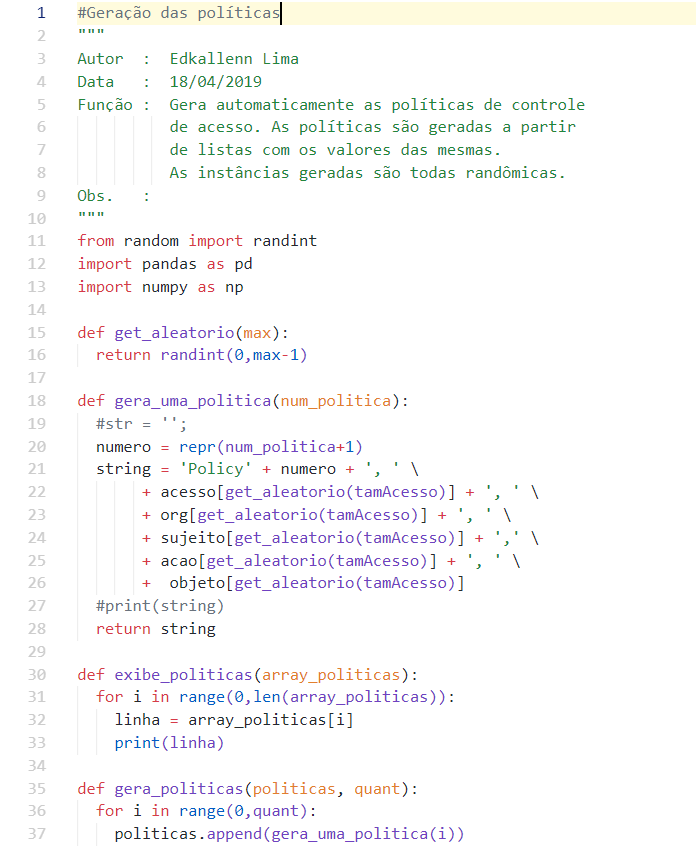
\includegraphics[width=.9\textwidth]{imagens/geracao-politicas-parte1.png}	}
	
	\label{fig:geracao-politicas-parte1}
	{\scriptsize Fonte: compilação do autor}
\end{figure}


Já as \autoref{fig:geracao-politicas-parte2} e \autoref{fig:geracao-politicas-part3} demonstra a segunda e a terceira partes do programa de geração de políticas.
\begin{figure}[h!]
	\centering
	\caption{Segunda parte do programa para geração de políticas automaticamente}
	\fbox{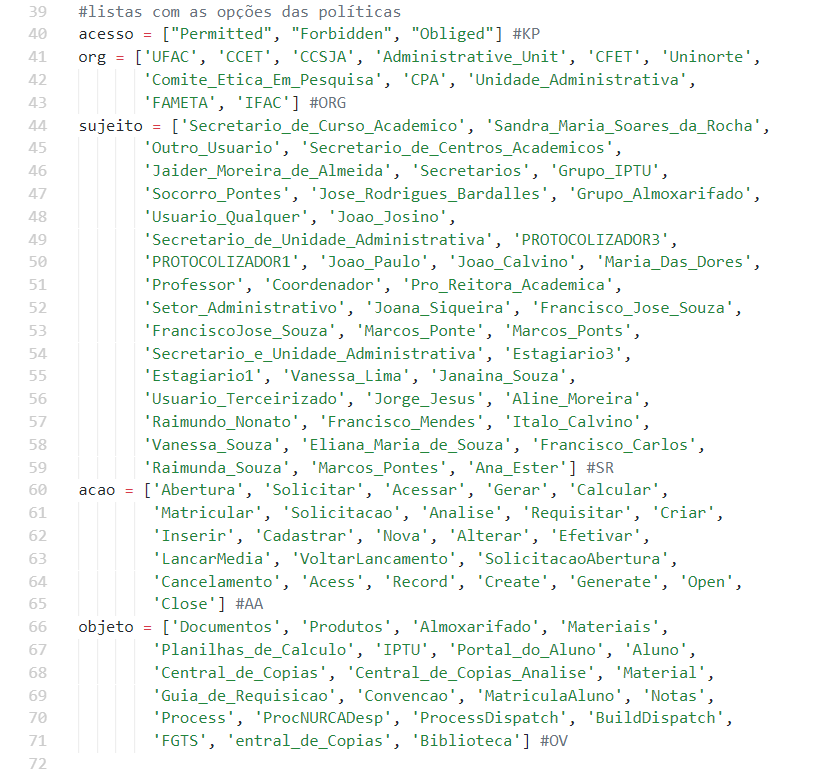
\includegraphics[width=.9\textwidth]{imagens/geracao-politicas-parte2.png}	}
	
	\label{fig:geracao-politicas-parte2}
	{\scriptsize Fonte: compilação do autor}
\end{figure}

\begin{figure}[h!]
	\centering
	\caption{Terceira Parte do programa para geração de políticas automaticamente}
	\fbox{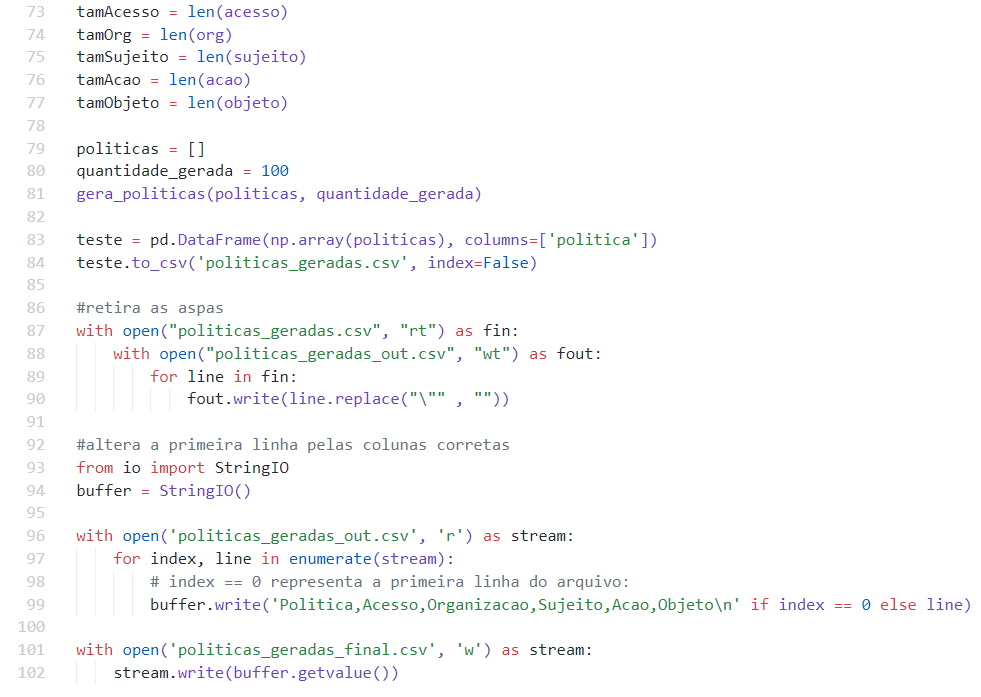
\includegraphics[width=.9\textwidth]{imagens/geracao-politicas-parte3.png}	}
	
	\label{fig:geracao-politicas-part3}
	{\scriptsize Fonte: compilação do autor}
\end{figure} 

Para os experimentos iniciais, um arquivo de políticas foi gerado randomicamente a partir do proposto em \citeonline{sarkis2017} e, de acordo com o exposto na \autoref{modelo_politica_utilizada}. O arquivo gerado possui, inicialmente, cerca de 68 políticas nomeadas (constituindo a \textit{fase de seleção}\footnote{cf. \autoref{mineracao_dados} deste trabalho.} da Mineração de Dados) e da fase coleta de dado do método proposto anteriormente. 

Este arquivo foi usado nos testes preliminares da hipótese descrita na \autoref{hipótese} deste trabalho. Para este problema da detecção de conflitos diretos serão usadas técnicas de aprendizagem supervisionada. Para tanto, ao arquivo com as políticas, no \textit{pré-processamento }foi acrescentada uma coluna rotulando os conflitos da seguinte forma: \textbf{1}: \textit{conflito direto} e \textbf{0}: \textit{sem conflito}. Esta estratégia é a mesma utilizada no trabalho de \citeonline{davy_application_2008} onde ele usa um modelo de matriz de controle de acesso usando operações lógicas \texttt{AND} e \texttt{OR} para identificação de conflitos.

A figura \ref{fig:aspecto_arquivo} demonstra o aspecto do arquivo das políticas geradas para os experimentos deste trabalho. Na imagem, pode-se notar a \textit{classe} (coluna) criada para guiar o aprendizado supervisionado dos algoritmos utilizados no estudo.

\begin{figure}[h!]
	\centering
	\caption{Aspecto do arquivo das políticas geradas para os experimentos}
	\fbox{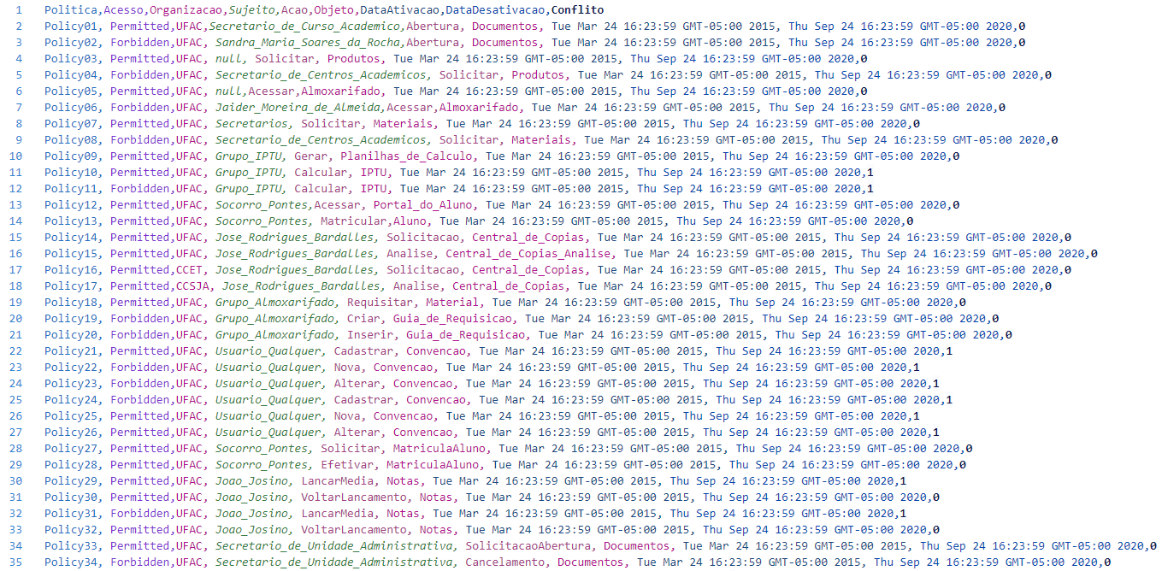
\includegraphics[width=1\textwidth]{imagens/aspecto_arquivo_politicas.png}	}
	
	\label{fig:aspecto_arquivo}
	{\scriptsize Fonte: compilação do autor}
\end{figure}

Ainda na fase de \textit{pré-processamento}, a coluna 9 (Conflito) foi transformada do tipo de dado \textit{Numérico para Nominal}. Para isso foi usado o softwate WEKA (descrito em \citeonline{eibe2016}) aplicado o filtro \textit{NumericToNominal} do software. Além disso, tanto o primeiro atributo quanto as datas de ativação e desativação da política foram removidos, pois, dentro do escopo estudado neste trabalho, eles não influenciariam nos resultados finais. O primeiro atributo é o ``nome'' da política, na forma ``PolicyXY'', onde XY é um número inteiro sequencial, iniciando em 1. O dataset, ao final, ficou com seis atributos, 5 previsores (Acesso, Organizacao, Sujeito, Acao e Objeto) e uma classe (o atributo `Conflito').

\subsection{Recursos computacionais}
Dois \textbf{ambientes computacionais} foram utilizados para as tarefas de mineração: um \textbf{notebook}  Intel Core i5 vPro-8350U (8ª Geração de 64 bits com 1.70GHz e 8 GB de RAM, com SSD de 256 GB rodando Windows 10 Pro.

O outro ambiente foi uma \textbf{Estação de Trabalho} Intel Core i7 vPro-6700 de 8ª geração de 64 bits com 3.40 Ghz e 20 GB de RAM, com HD de 1 TB rodando o Windows 10 Pro.

\subsection{Experimentos iniciais - arquivo com 68 políticas}\label{exp:iniciais}
O arquivo de 68 políticas criado com o programa descrito em \ref{fig:geracao-politicas-parte1} está disponível no endereço: \hyperlink{https://bit.ly/3io2PJf}{https://bit.ly/3io2PJf}.
%dataset-68 
A \autoref{fig:dataset-68 } mostra como ficou o arquivo com 68 políticas após a execução do pré-processamento.
\begin{figure}[h!]
	\centering
	\caption{Aspecto do arquivo com 68 políticas após o pré-processamento}
	\fbox{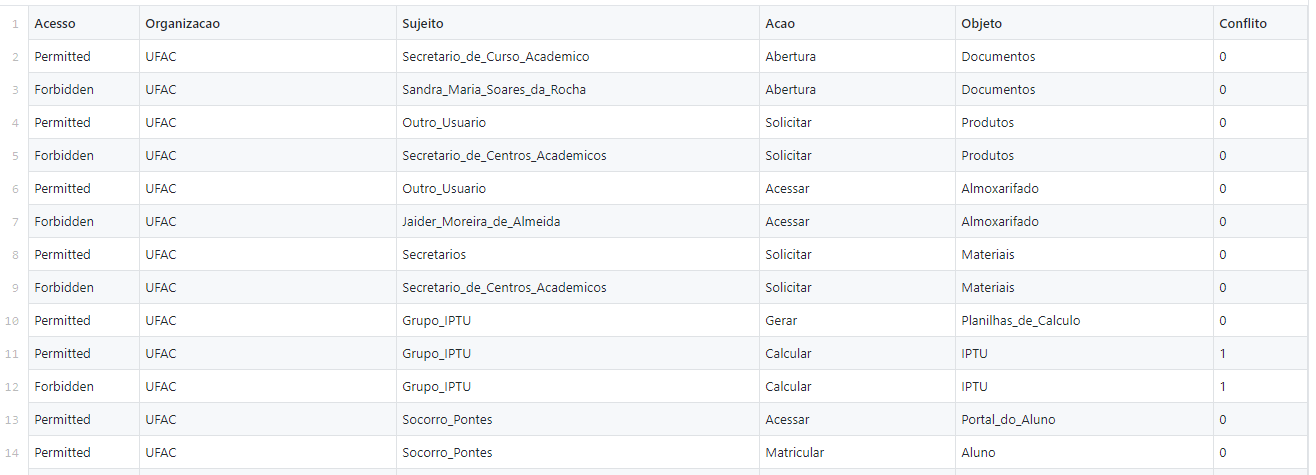
\includegraphics[width=1\textwidth]{imagens/dataset-68.png}	}
	
	\label{fig:dataset-68 }
	{\scriptsize Fonte: compilação do autor}
\end{figure}



\subsection{Resultados - Arquivo com 68 políticas}
Logo após, experimentos foram realizados de forma preliminar no \textit{dataset} envolvendo os diversos algoritmos com alguns parâmetros sendo alterados (a maioria com pequena ou nenhuma variação) para se chegar às técnicas finais que foram utilizadas nos posteriores experimentos e que serão explicitadas a seguir.

Utilizando-se a ferramenta WEKA descrita em \cite{eibe2016} para as últimas fases da Mineração de Dados, foram utilizados alguns algoritmos de classificação que segundo \citeonline{wu2007} são alguns dos mais utilizados na Mineração de Dados. Para avaliar o desempenho definiu-se o método \textit{cross-validatio}n com 10 folds. Em seguida suas acurácias foram comparadas.

A tabela \ref{tab:acuracias} mostra o resultado destes experimentos:
\begin{table}[h!]
	\centering
	\caption{Acurácia dos classificadores}
	\label{tab:acuracias}
	\vspace{0.3cm}
	\begin{tabular}{p{6cm}c}
		\hline\\
		Classificador/Algoritmo& Acurácia  \\[10pt] 
		\hline
		Multi Layer Perceptron & 0.9705    \\
		SVM kernel linear~     & 0.9705    \\
		Random Forest~		   & 0.9542	   \\
		J48                    & 0.9411    \\
		K* (K-star)            & 0.9411    \\
		Trees LMT              & 0.9117    \\
		IBk (KNN, com k =1)~   & 0.8970    \\
		JRip                   & 0.8970    \\		
		Nayve Bayes            & 0.8674    \\
		Random Tree            & 0.7794    \\
		\hline
	\end{tabular}
	\\[6pt]	\centering {\footnotesize Fonte: Elaborada pelo autor mediante experimentos}	
\end{table}

As figuras \ref{fig:saida_svm} e \ref{fig:saida_multilayerperceptron} mostram os resultados das classificações do arquivo de políticas usando, respectivamente, os classificadores/algoritmos: \textit{SVM} e o \textit{MultiLayer Perceptron} (que foram os principais citados nos trabalhos relacionados, cf. descrito na \autoref{trabalhos_relacionados}). Cf. mostrado na \autoref{tab:acuracias}, os classificadores SVM e MultiLayerPerceptron ficaram empatados em relação à acurácia. Provavelmente, a base pequena possa ter, de alguma forma, influenciado no resultado.
\begin{figure}[h!]
	\centering
	\caption{Saída do software WEKA. Classificador: SVM}
	\fbox{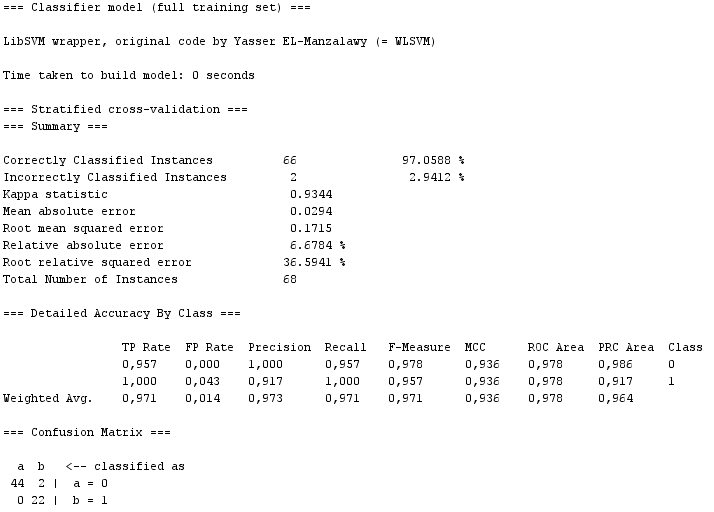
\includegraphics[width=.7\textwidth]{imagens/svm-resultados.png}	}

	\label{fig:saida_svm}
	{\scriptsize Fonte: compilação do autor}
\end{figure}
\begin{figure}[h!]
	\centering
	\caption{Saída do software WEKA. Classificador: \textit{MultiLayer Perceptron}}
	\fbox{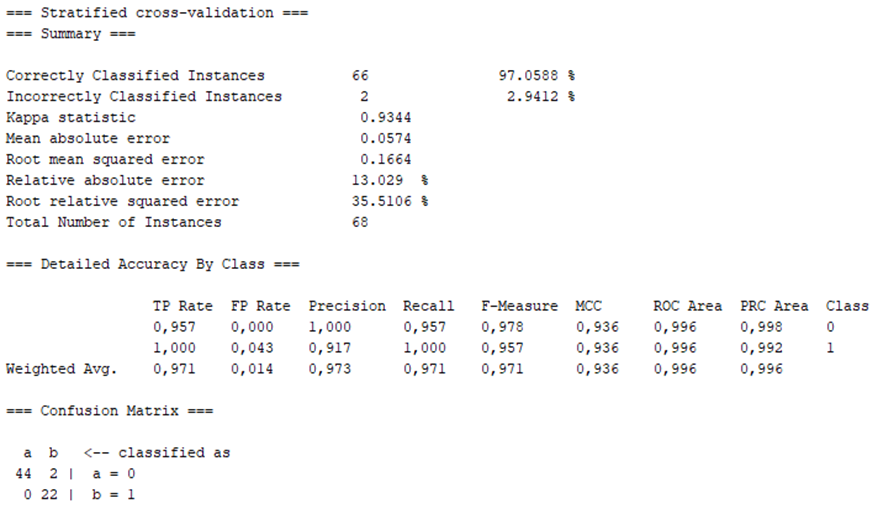
\includegraphics[width=.7\textwidth]{imagens/multilayerperceptron-resultados.png}}
 
	\label{fig:saida_multilayerperceptron}
	{\scriptsize Fonte: compilação do autor}
\end{figure}

Assim, com uma acurácia de 97,05\% na classificação dos conflitos diretos, tanto o algoritmo Multilayer Perceptron (que implementa uma rede neural sigmoide multicamadas) quanto o SVM tiveram a maior acurácia, com 95,7\% de \textit{TP rate}(taxa de \textit{True Positives} ou verdadeiros positivos) para a classe 0 (não há conflito) e, somente, 4,3\% de \textit{FP rate}(taxa de Falsos Positivos) para a classe 1 (quando há conflito direto). Nos experimentos realizados (assim como se esperava inicialmente na hipótese deste trabalho --- baseado em evidências da literatura), estes modelos algorítmicos foram os mais eficientes para a detecção de conflitos diretos.

A interface visual do WEKA é interessante para observar o comportamento inicial dos algoritmos, mas para as arquiteturas de redes neurais e seus diversos parâmetros, configurações e quantidade de camadas ocultas, entre outras configurações levaram a outros experimentos com outras abordagens. Para isso e com o objetivo de evitar o \textit{overfitting}, como explicado na \autoref{medidas_avaliacao} novos procedimentos e ferramentas foram adotados, incluindo, alterando a estratégia de validação.

\section{Outros experimentos - arquivos com 281 e 430 políticas}\label{exp:139-281}
Foi gerado, então, dois novos arquivos de políticas, também randomicamente, e, ainda, a partir do proposto em \citeonline{sarkis2017} e, cf. o exposto na \autoref{modelo_politica_utilizada} usando o software demonstrado em \ref{fig:geracao-politicas-parte1}. Os arquivos gerados agora, possui, 281 e 430 políticas nomeadas. O arquivo de 281 políticas está disponível em \hyperlink{https://bit.ly/2MW1GwA}{https://bit.ly/2MW1GwA}.

\begin{figure}[h!]
	\centering
	\caption{Parte do arquivo com 281 políticas após o pré-processamento}
	\fbox{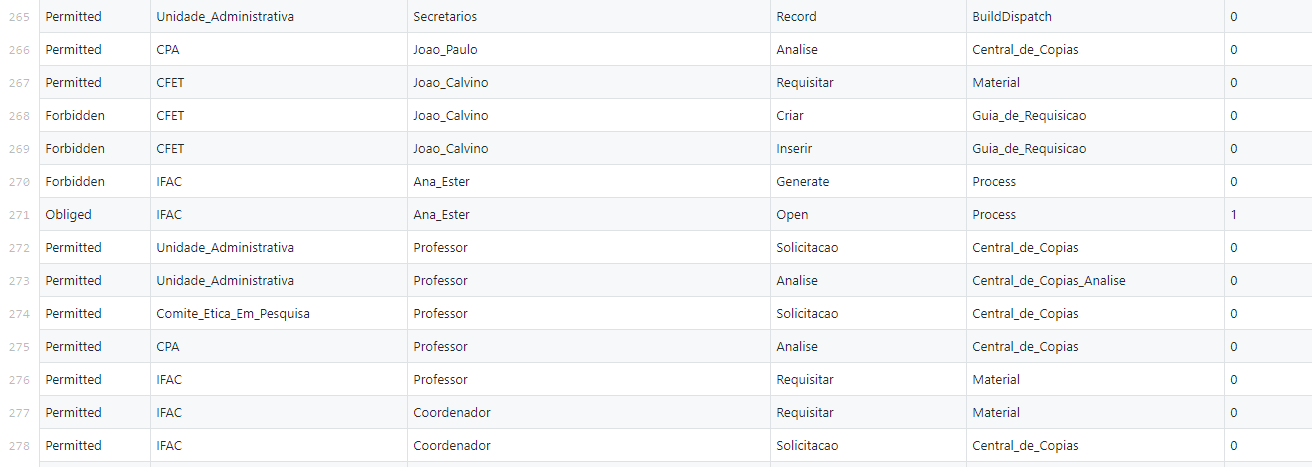
\includegraphics[width=.8\textwidth]{imagens/dataset-281.png}}
	
	\label{fig:dataset-281}
	{\scriptsize Fonte: compilação do autor}
\end{figure}

Os mesmos filtros anteriores foram aplicados:\begin{itemize} \label{filtros}
	\item a coluna 9 (Conflito) foi transformada do tipo de dado \textit{Numérico para Nominal}. Este atributo é a classe;
	\item O primeiro atributo, o ``nome'' da política, na forma ``PolicyXY'', onde XY é um número inteiro sequencial, iniciando em 1 foi removido;
	\item Tanto as datas de ativação quanto de desativação da política foram removidas;
	\item O dataset, ao final, ficou com seis atributos, 5 previsores (Acesso, Organizacao, Sujeito, Acao e Objeto) e uma classe (o atributo `Conflito').
\end{itemize}

Os resultados para os algoritmos (ainda usando a ferramenta Weka) foram os seguintes:

Para o MultiLayer Perceptron, a \autoref{tab:MLP_acuracia} mostra como as acurácias ficaram com os arquivos com quantidades diferentes de políticas.

\begin{table}[h!]
	\centering
	\caption{Acurácia do MLP}
	\label{tab:MLP_acuracia}
	\vspace{0.3cm}
	\begin{tabular}{p{6cm}c}
		\hline\\
		Qtd. de Políticas	& Acurácia  \\[10pt] 
		\hline
		68 					& 97.05    	\\
		281			     	& 98.73     \\
		430					& 99.28		\\
		\hline
	\end{tabular}
	\\[6pt]	\centering {\footnotesize Fonte: Elaborada pelo autor mediante experimentos}	
\end{table}

Para o classificador SVM, a \autoref{tab:SVM_acuracia} mostra como as acurácias ficaram com os arquivos com quantidades diferentes de políticas.

\begin{table}[h!]
	\centering
	\caption{Acurácia do SVM}
	\label{tab:SVM_acuracia}
	\vspace{0.3cm}
	\begin{tabular}{p{6cm}c}
		\hline\\
		Qtd. de Políticas	& Acurácia  \\[10pt] 
		\hline
		68 					& 97.05    	\\
		281		     	& 96.40     \\
		430					& 99.28		\\
		\hline
	\end{tabular}
	\\[6pt]	\centering {\footnotesize Fonte: Elaborada pelo autor mediante experimentos}	
\end{table}

Mesmo com uma leve queda na acurácia do SVM no arquivo de 281 políticas, percebe-se que, quanto maior o número de políticas, é crescente a acurácia do classificador e, portanto, melhor é a classificação.

\subsection{Experimentos com Pandas, NumPy e sklearn - arquivo de 430 políticas}\label{exp:pandas-numpy-sklearn}
Outros experimentos foram realizados utilizando as bibliotecas Pandas, descrita em \citeonline{pandas-mckinney2010}, NumPy, pormenorizada em \citeonline{numpy-oliphant2006guide} e sklearn, detalhado em \citeonline{scikit-learn} além do Notebook Jupyter, caracterizado em \citeonline{jupyter-Kluyver:2016aa}. 

O notebook criado demonstra o treinamento de uma rede neural Rede Neural Multicamadas usando o classificador \texttt{\textbf{MLPClassifier}} da biblioteca \texttt{\textbf{sklearn}}.

No arquivo, é demonstrado os experimentos na construção de uma arquitetura de uma rede neural com a estratégia de testes \textit{holdout} sendo a divisão da base (split) em atributos previsores e classe com cerca de 75\% da base sendo usada para treinamento da rede e 25\% para teste.

Há também um pré-processamento importante focado em um tratamento dos dados categóricos do \textit{dataset} e sua conversão para dados numéricos e divisão da base original em dois conjuntos de dados (previsores e classe).

Todos os atributos categóricos do dataset de políticas (o maior, com 430 instâncias) foram transformados para numéricos sendo um dicionário de dados construído para isso utilizando uma técnica chamada codificação, semelhante à da classe LabelEncoder da biblioteca \texttt{sklearn}. Basicamente, o processo codifica rótulos de destino com valores entre $0$ e $n$-classes $- 1$. Isto é importante, pois alguns algoritmos só trabalham com valores numéricos (como o MultiLayerPerceptron, o SVM entre outros).

Os passos foram os seguintes:

Primeiramente a base foi importada da seguinte forma, como demonstrado na \autoref{fig:base-head} mostrando o aspecto inicial do dataset.

\begin{figure}[h!]
	\centering
	\caption{Aspecto do dataset importado}
	\fbox{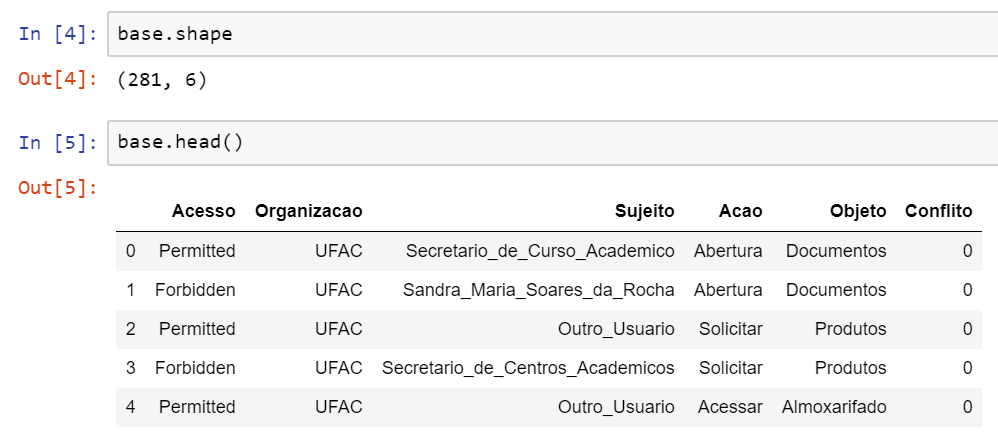
\includegraphics[width=.6\textwidth]{imagens/notebook-base1.png}}
	
	\label{fig:base-head}
	{\scriptsize Fonte: compilação do autor}
\end{figure}

A partir daí, foram selecionados da base todas as linhas dos atributos do \textit{dataset} que estavam com os tipos \textit{object}. Foram procurados valores nulos e não foram encontrados. 

Foi utilizada uma técnica que transforma um atributo categórico com $k$ valores em uma representação numérica com valores inteiros para cada $k$ valor chamada \textit{label encoder}, ou seja, ela codifica os rótulos de destino com valores entre $1$ e $n$-classes$-1$. Há vantagens e desvantagens nessa abordagem. Elas estão discutidas em detalhes em \citeonline{sarkar_2017}.

A \autoref{fig:dic-coluna1} demonstra como este procedimento foi realizado para o atributo que representa o acesso (Permitido, Proibido e Obrigatório).

\begin{figure}[h]
	\centering
	\caption{Engenharia de atributos - dados categóricos textuais}
	\fbox{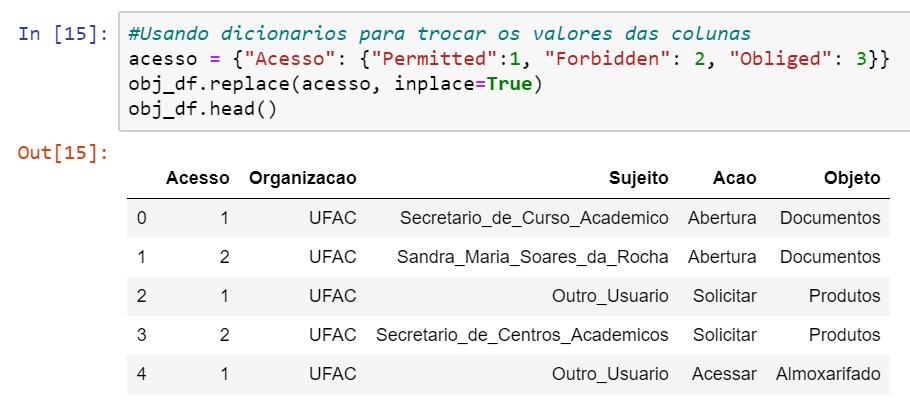
\includegraphics[width=.6\textwidth]{imagens/notebook-base2.png}}
	
	\label{fig:dic-coluna1}
	{\scriptsize Fonte: compilação do autor}
\end{figure}

Uma função para realizar o encode automático foi criada. Ela está disponível em \hyperlink{https://bit.ly/3qoILsX}{https://bit.ly/3qoILsX}.

Em seguida a base foi dividida em atributos previsores e a classe. Os previsores são as colunas que representam a política em si e a classe é a representação binária do conflito.

\begin{figure}[H]
	\centering
	\caption{Aspecto dos atributos previsores}
	\fbox{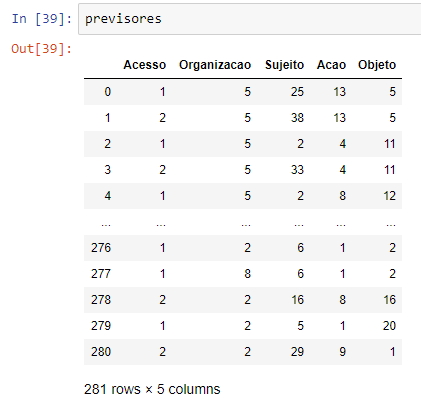
\includegraphics[width=.6\textwidth]{imagens/previsores.png}}
	
	\label{fig:previsores}
	{\scriptsize Fonte: compilação do autor}
\end{figure}

O aspecto dos atributos previsores ficou como o mostrado na \autoref{fig:previsores}. Já a classe ficou com o aspecto da \autoref{fig:classe}.

Em seguida os atributos foram transformados usando padronização para manter as variáveis na mesma ordem de grandeza. Na padronização, a média se iguala a 0 e o desvio-padrão se mantém em 1. A fórmula da padronização é a seguinte:

\begin{equation}\label{eq:padronizacao}
z = \frac{x - \mu}{\sigma}
\end{equation}

onde $\mu$ é a média aritmética e $\sigma$ é o desvio-padrão dos dados. Como todos os dados estão agora em formato numérico, é um passo importante. 

O código para a padronização foi o \autoref{padronizacao}, abaixo:
\begin{lstlisting}[caption={Código da Padronização},label=padronizacao][frame=single][language=Python]
	from sklearn.preprocessing import StandardScaler
	scaler = StandardScaler()
	previsores_transformados = scaler.fit_transform(previsores)
\end{lstlisting}

Assim os dados foram padronizados e ficaram na mesma escala. Todos os algoritmos que foram padronizados utilizaram este mesmo algoritmo. Foi gerado, então um novo conjunto de dados de treinamento com 75\% do \textit{dataset} (sendo escolhidos randomicamente). Deixando, assim, 25\% da base para validação.

\begin{figure}[H]
	\centering
	\caption{Aspecto do atributo classe}
	\fbox{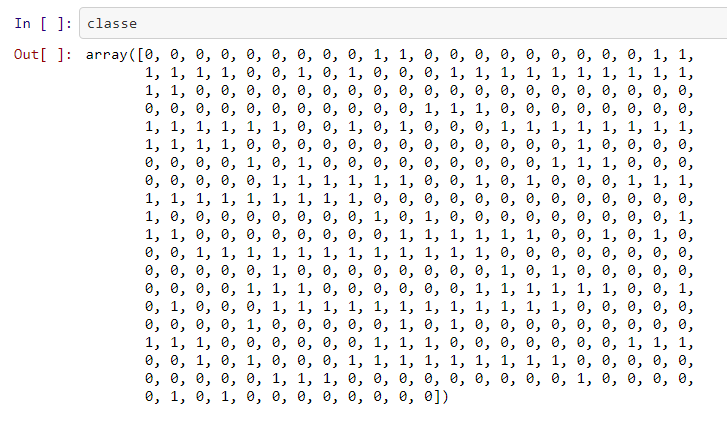
\includegraphics[width=.8\textwidth]{imagens/classe2.png}}
	
	\label{fig:classe}
	{\scriptsize Fonte: compilação do autor}
\end{figure}

Logo em seguida, um modelo de Multi-Layer Perceptron foi criado usando o classificador \texttt{\textbf{MLPClassifier}} da biblioteca \texttt{\textbf{sklearn}} com os seguintes hiperparâmetros, mostrados no \autoref{hiperMLP}: 
%[caption={Hiperparâmetros do modelo MLPClassifier}, label=hiperMLP][frame=single]
\begin{lstlisting}[caption={Hiperparâmetros do MLPClassifier},label=hiperMLP][frame=single][language=Python]
	verbose = True,
	max_iter=10000,
	tol = 0.000010,
	solver = 'adam',
	hidden_layer_sizes=(32),
	shuffle=False,
	activation='relu' ,
	batch_size=40
\end{lstlisting}

%\begin{itemize}
	%\item \texttt{$max\textunderscore iter=10000$,}
	%\item \texttt{$tol = 0.0000010$,}
	%\item \texttt{$solver = 'adam'$,}
	%\item \texttt{$hidden\textunderscore layer\textunderscore sizes=(100)$ ,}
	%\item \texttt{$shuffle=False$,}
	%\item \texttt{$activation='relu'$}
%\end{itemize}

Onde, respectivamente estão configuradas, o número máximo de épocas de treinamento (10000), a tolerância (0.000010), a função de otimização de peso (`adam' refere-se a um otimizador estocástico baseado em gradiente descendente), a quantidade de neurônios na única camada oculta, se as amostras devem ser embaralhadas em cada iteração (marcado como falso) e a função de ativação da camada oculta (função de ativação ReLU).

A \autoref{fig:mlp_classifier} mostra o código no notebook e as iterações finais onde o classificador indica que a função de perda no treinamento não melhorou mais do que a tolerância, $tol = 0.000010$ por 10 épocas consecutivas e, portanto, ele encerrou as iterações.

\begin{figure}[h]
	\centering
	\caption{Código do \textbf{MLPClassifier} com as primeiras iterações}
	\fbox{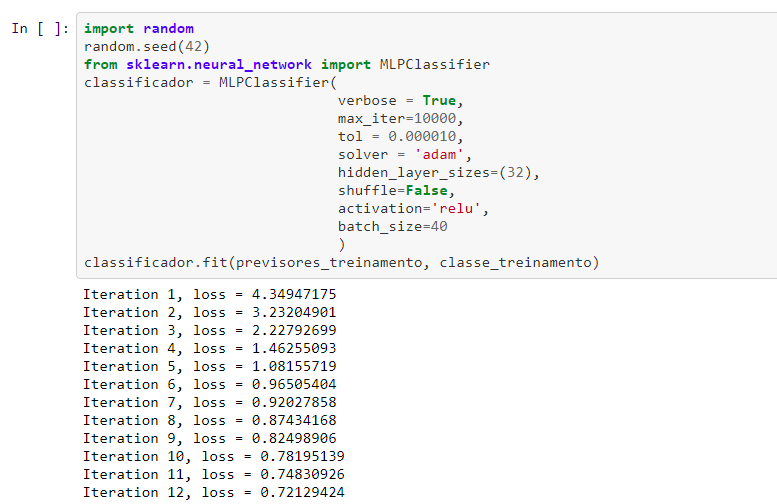
\includegraphics[width=.8\textwidth]{imagens/mlp_classifier2.png}}
	
	\label{fig:mlp_classifier}
	{\scriptsize Fonte: compilação do autor}
\end{figure}

A \autoref{fig:validacao_notebook} mostra algumas métricas de validação após o modelo criado realizar as predições na base de teste (25\% do dataset ou 71 políticas). Nela, pode-se perceber a acurácia do classificador em 95.77\%, classificando, conforme a matriz de confusão mostrada na mesma figura, somente 3 previsões incorretas. Estes resultados apresentam uma sensibilidade (\textit{recall}) de 97.7\%. Levando-se em conta que o modelo se aprimora conforme a quantidade de instâncias aumenta, de acordo com o pressuposto no\textit{ teorema da aproximação universal} \citeonline{hagan_neural_1996}, pode se considerar este como um modelo satisfatório.

\begin{figure}[h]
	\centering
	\caption{Validações para o modelo \textbf{MLPClassifier}}
	\fbox{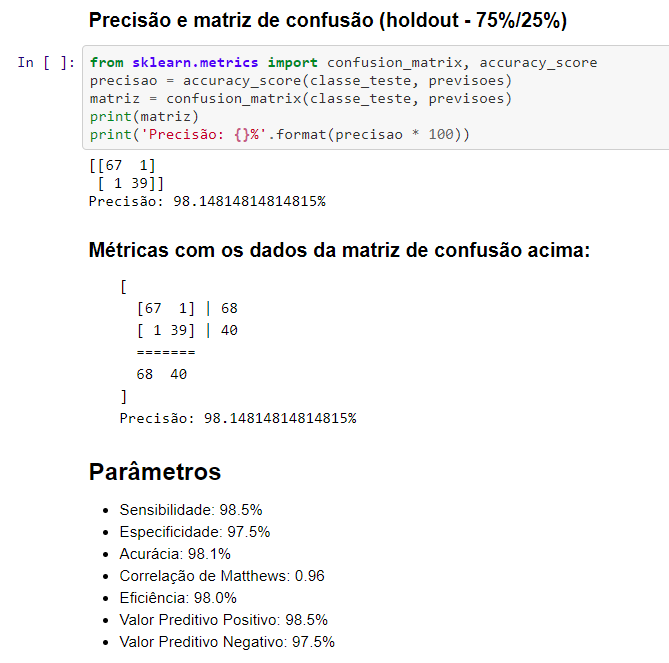
\includegraphics[width=.7\textwidth]{imagens/validacao_notebook2.png}}
	
	\label{fig:validacao_notebook}
	{\scriptsize Fonte: compilação do autor}
\end{figure}

%mlp-convergencia-perda

Já a figura \autoref{fig:mlp-convergencia-perda} mostra a convergência da função de perda.

\begin{figure}[h]
	\centering
	\caption{Convergência da Loss Function - \textbf{MLPClassifier}}
	\fbox{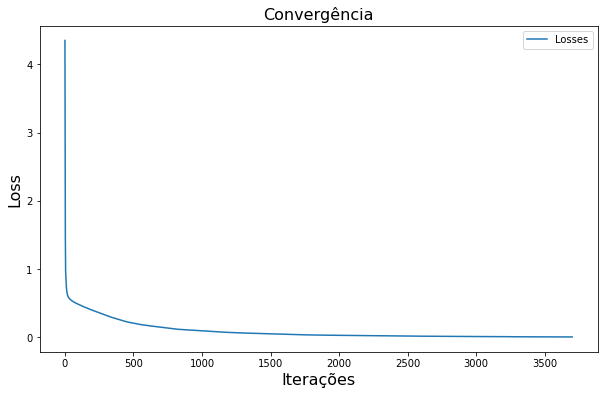
\includegraphics[width=.6\textwidth]{imagens/mlp-convergencia-perda.png}}
	
	\label{fig:mlp-convergencia-perda}
	{\scriptsize Fonte: compilação do autor}
\end{figure}

A \autoref{fig:dimensionalidade} mostra a dimensionalidade dos dados após transformados pelo processo de padronização e dá uma visão geral de 3 atributos, \textit{\textbf{sujeito, ação e objeto}} e o impacto na difusão dos conflitos no espaço após os atributos categóricos terem sido, todos, transformados para uma representação numérica.

\begin{figure}[h]
	\centering
	\caption{Dimensionalidade dos dados: atributos sujeito, ação e objeto}
	\fbox{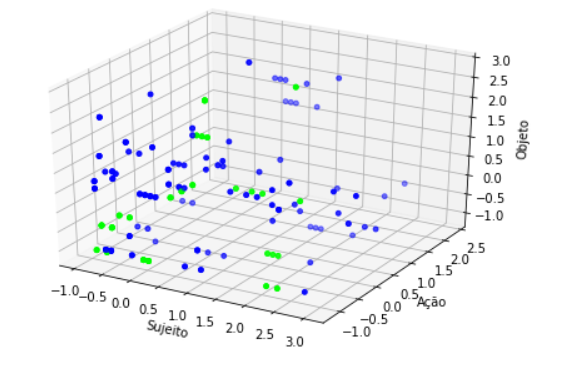
\includegraphics[width=.6\textwidth]{imagens/dimensionalidade.png}}
	
	\label{fig:dimensionalidade}
	{\scriptsize Fonte: compilação do autor}
\end{figure}


Foi criado um script que, com parâmetros padrão dos classificadores, roda um experimento sobre a base. O script esá disponível em \hyperlink{https://bit.ly/3bFJaTM}{https://bit.ly/3bFJaTM}. O resultado pode ser visualizado na \autoref{fig:comparacao-visual}.

%comparacao-visual
\begin{figure}[h]
	\centering
	\caption{Comparação visual entre alguns classificadores}
	\fbox{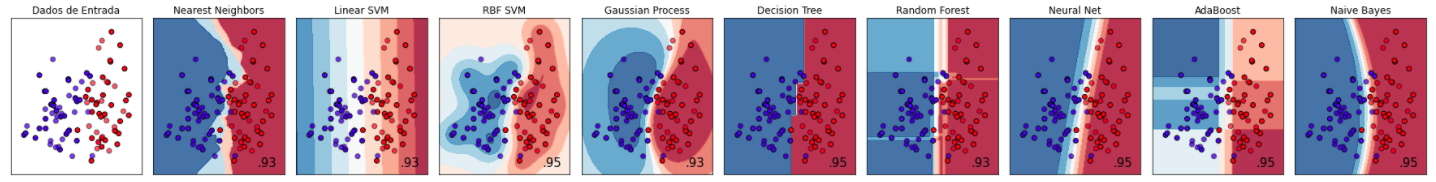
\includegraphics[width=1\textwidth]{imagens/comparacao-visual.png}}
	
	\label{fig:comparacao-visual}
	{\scriptsize Fonte: compilação do autor}
\end{figure}

O notebook com todos os experimentos restantes (Naïve Bayes, Keras, K-NN, SVM, Random Forest e Árvores de Decisão) pode ser visualizado em \hyperlink{https://bit.ly/3nJHYky}{https://bit.ly/3nJHYky}. Na \autoref{tab:acuracias2} com as acurácias destes classificadores conforme ficou demonstrada nos experimentos.

\begin{table}[h]
	\centering
	\caption{Acurácia dos classificadores - dataset 430 políticas}
	\label{tab:acuracias2}
	\vspace{0.3cm}
	\begin{tabular}{p{6cm}c}
		\hline\\
		Classificador/Algoritmo& Acurácia  \\[10pt] 
		\hline
		Random Forest~		   & 0.9900    \\
		Árvore de Decisão      & 0.9900    \\
		MLPCLassifier~		   & 0.9814   \\
		SVM RBF                & 0.9814    \\
		Keras (MLP)            & 0.9629    \\
		k-NN (com k=5          & 0.8796    \\
		SVM kernel linear~	   & 0.8055    \\
		Naïve Bayes~		   & 0.7314    \\		
		\hline
	\end{tabular}
	\\[6pt]	\centering {\footnotesize Fonte: Elaborada pelo autor mediante experimentos}	
\end{table}

\subsection{Experimentos com TensorFlow e Pytorch}\label{exp:tensorflow-pytorch}
De acordo com \citeonline[p. 233]{geron_maos_2020}, o \textit{TensorFlow} é uma biblioteca de software para cálculo numérico de código aberto especialmente adequada e ajustada para o Aprendizado de Máquina em larga escala. Foi desenvolvido pela \textit{Google Brain Team} para uso intensivo de redes neurais profundas. O código fonte foi liberado em 2015 e está à disposição no link: \hyperlink{https://github.com/tensorflow/tensorflow}{https://github.com/tensorflow/tensorflow}.

É possível usar computação paralela em várias CPU's ou GPU's além de suportar computação distribuída para que seja possível o treinamento e o uso de redes neurais em grandes conjuntos de treinamento dividindo os cálculos por centenas de servidores em um período de tempo razoável \cite{geron_maos_2020}. 

Entre suas características importantes destacam-se: rodar em diversos sistemas operacionais (e inclusive na nuvem); diversas APIs públicas para criação, treinamento e avaliação de arquiteturas de diferentes tipos de redes neurais; diversas outras API's de alto nível foram construídas com base no TensorFlow como o \textit{Keras} e o \textit{Pretty Tensor}; implementações em C++ altamente eficientes para operações de Aprendizado de Máquina; nós de otimização avançados para procura por parâmetros que minimizem uma função de custo; usa extensões CUDA, uma  API destinada a computação paralela, GPGPU, e computação heterogênea, criada pela Nvidia que dá acesso ao conjunto de instruções virtuais da GPU e a elementos de computação paralela \cite{geron_maos_2020}.

Os cálculos no \textit{TensorFlow} são expressos como grafos de fluxo de dados , seu nome deriva das operações que as redes neurais realizam em arranjos de dados multidimensionais, chamados de ``tensores''(generalização matemática de escalares, vetores e matrizes) \cite{kadimisetty_tensorflow_2018}.

Foi realizado, assim, no escopo deste trabalho experimentos com a base de dados de com 281 políticas já citada anteriormente. O notebook completo está disponível online no endereço: \underline{\texttt{https://bit.ly/33BmCzt}}. Foi todo construído no ambiente Google Collab que é um serviço de nuvem gratuito hospedado pelo Google para incentivar a pesquisa de Aprendizado de Máquina e Inteligência Artificial, similar ao Jupyter Notebook, é uma lista de células que podem conter textos explicativos ou códigos executáveis e suas saídas \cite{collab_2020}.

Neste modelo os hiperparâmetros principais, cf. \citeonline{thenmozhi_multi-lingual_2018} foram ajustados como: tamanho do batch em 20 (analisa, computa e reajusta os pesos de 20 instâncias de cada vez, por época), o número de GPU's trabalhando em conjunto para 4, a taxa de aprendizado em 0.00001, o decaimento dos pesos em 0.000005 e o número de épocas padrão em 30 (apenas para testes inciais).

\begin{figure}[h!]
	\centering
	\caption{Separação dos dados de teste e treino}
	\fbox{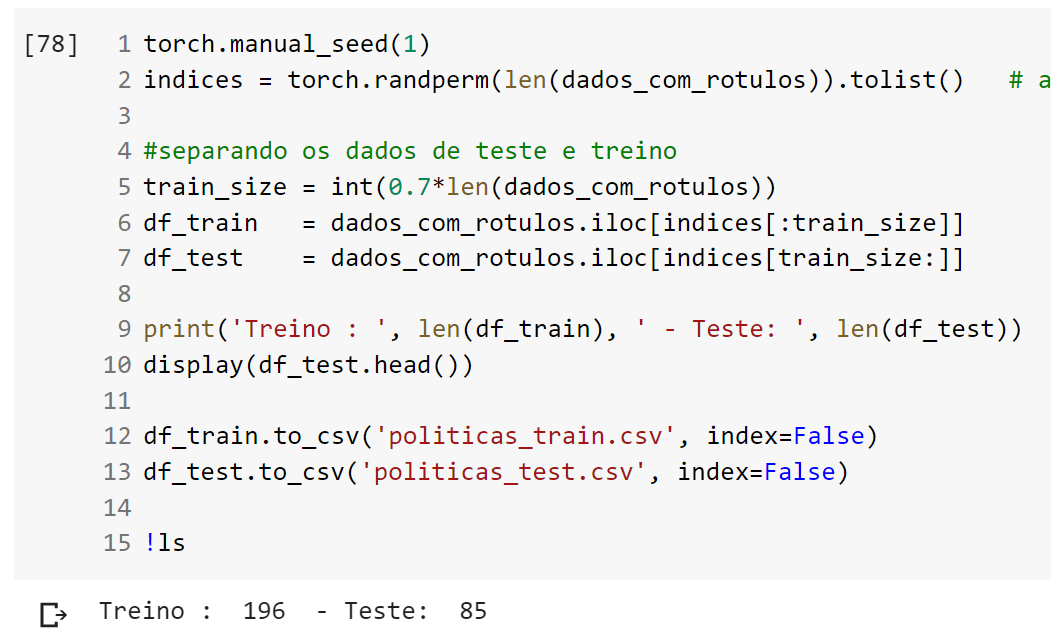
\includegraphics[width=.6\textwidth]{imagens/separacao-teste-treino.png}}
	
	\label{fig:separacao-teste-treino}
	{\scriptsize Fonte: compilação do autor}
\end{figure}

Para o processo de validação, usou-se o \textit{holdout} com a separação em 75\% das instâncias para o treinamento da rede neural e 25\% para teste, predição e validação. Na figura \ref{fig:separacao-teste-treino} pode-se visualizar como o processo foi realizado,inclusive com a quantidade de instâncias em cada conjunto de dados (na linha 2 é feita a randomização do \textit{dataset} original para evitar o overfitting e balancear a probabilidade da distribuição).

O pacote \texttt{torch.util.data} do PyTorch possui a classe abstrata \texttt{Dataset}. Ela permite que seja implementado o próprio dataset reescrevendo os métodos: 

\begin{itemize}	
	\item \verb|__init__(self)|: Define a lista de amostras do dataset
	\item \verb|__getitem__(self, idx)|: Carrega uma amostra, aplica as devidas transformações e retorna uma tupla (dado, rótulo)
	\item \verb|__len__(self)|: Retorna a quantidade de amostras do dataset
\end{itemize}

Dessa forma, a \autoref{fig:classe-politicas} mostra a elaboração de uma classe chamada \texttt{Politicas} que implementa uma classe-filha que herda da superclasse, \textit{Dataset} descrita acima.

\begin{figure}[h!]
	\centering
	\caption{Implementação da classe Politicas}
	\fbox{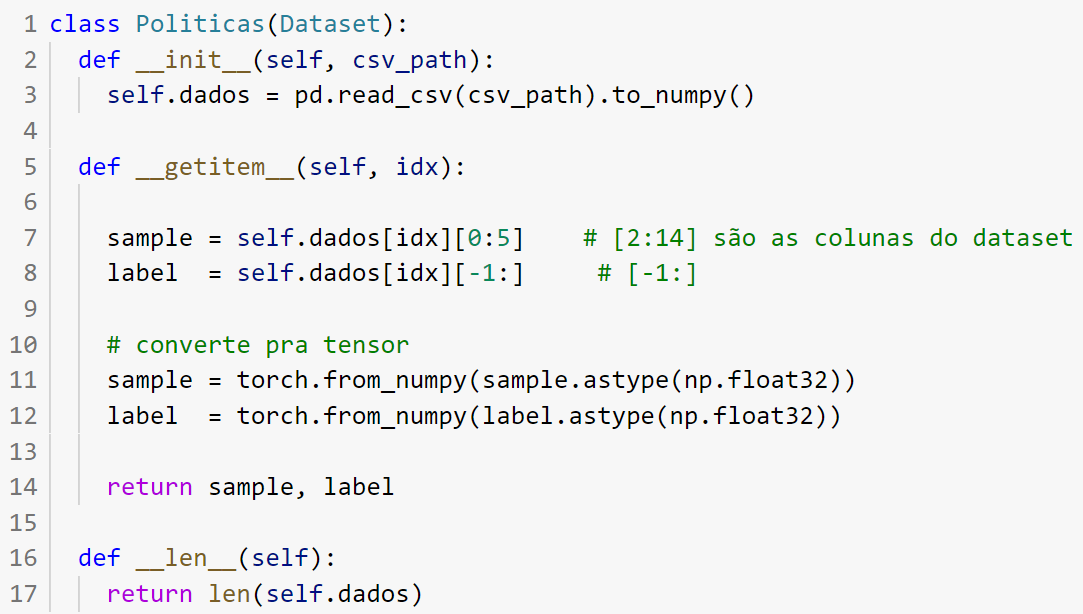
\includegraphics[width=.6\textwidth]{imagens/classe-politicas.png}}
	
	\label{fig:classe-politicas}
	{\scriptsize Fonte: compilação do autor}
\end{figure}

Em seguida, dois objetos DataLoader são criados, um para a base de treinamento e um para a base de teste. Em seguida, a Rede Neural Multicamadas é instanciada mediante a criação de uma classe chamada MLP que herda da classe \texttt{nn.Module} que representa um módulo genérico de uma rede neural. 

A arquitetura da rede é configurada dentro da classe que a cria sendo: uma\textit{ camada linear} de entrada, duas \textit{camadas lineares ocultas com 32 neurônios} em cada camada usando a função de ativação ReLU e \textit{uma camada linear de saída com dois neurônios}, representando os dois rótulos do atributo que é a classe, neste caso específico, o atributo binário \textbf{conflito} que será predito. 

É criada, no mesmo código da classe MLP, uma função que faz o avanço (fed-forward) das computações na rede e, ao final, é instanciada uma variável chamada \texttt{\textbf{net}} com as variáveis descritas: 
\begin{itemize}
	\item 5 atributos/neurônios na camada linear de entrada;
	\item 2 camadas ocultas com 32 neurônios cada; e
	\item 2 camadas de saída representando as variáveis preditas
\end{itemize}

Na mesma linha que cria o objeto \texttt{net} é feito o \textit{cast} da rede na GPU para que ela possa, ao ser treinada, fazer uso dos poderes computacionais em paralelo da API, CUDA. A \autoref{fig:mlp-pytorch} mostra o código descrito aqui.

Em seguida é definida uma \textit{loss function}(função de perda ou de custo). É criado um critério que mede o erro médio quadrático (norma matricial ao quadrado) entre cada elemento na entrada $x$ e o destino $y$, cf. \autoref{erro_quadratico_medio} da página \autopageref{erro_quadratico_medio}. 

O otimizador utilizado é o Adam, um algoritmo para otimização estocástica descrito em \citeonline{adam_2017} passando para o algoritmo os valores da taxa de aprendizado e do decaimento de pesos mostrado anteriormente nesta seção.

\begin{figure}[H]
	\centering
	\caption{Implementação da classe que modela a arquitetura da rede}
	\fbox{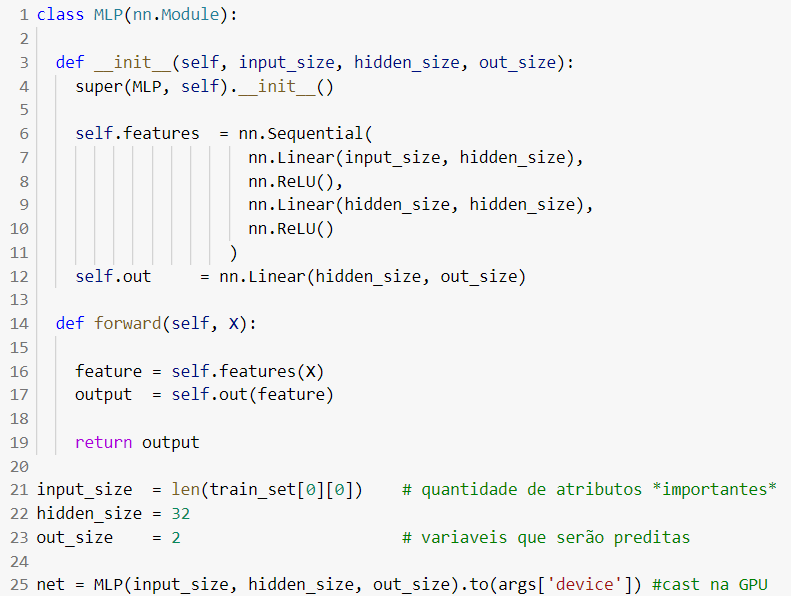
\includegraphics[width=.6\textwidth]{imagens/mlp-pytorch.png}}
	
	\label{fig:mlp-pytorch}
	{\scriptsize Fonte: compilação do autor}
\end{figure}

O fluxo de treinamento desta arquitetura de rede neural multicamadas proposta neste experimento segue o algoritmo iterativo:

\begin{itemize}
	\item Iterar nas épocas
	\item Iterar nos batches (a quantidade de instâncias simultâneas)
	\item Cast dos dados no dispositivo de hardware (GPU)
	\item Forward na rede e cálculo da \textit{loss function}
	\item Cálculo do gradiente e atualização dos pesos
\end{itemize}

Esse conjunto de passos é responsável pelo processo iterativo de otimização de uma rede. A validação, entretanto, é apenas a aplicação da rede em dados nunca antes vistos para estimar a qualidade do modelo no mundo real.

Três funções, portanto, são criadas, uma para modelar o treinamento da rede neural, uma para o teste e validação e outra que agrega as duas primeiras em uma só para executar o algoritmo descrito anteriormente. Então, para finalizar o experimento com o TensorFlow, o PyTorch, CUDA e o Google Collaboratory, \textit{foi realizado um treinamento com 500 épocas da rede neural} explanada nesta seção e os resultados tanto do treino quando do teste e validação foram armazenados.

As figuras \ref{fig:train}, \ref{fig:test} e \ref{fig:forward} mostram as três funções citadas anteriormente.

\begin{figure}[H]
	\centering
	\caption{Implementação da função de treino da rede}
	\fbox{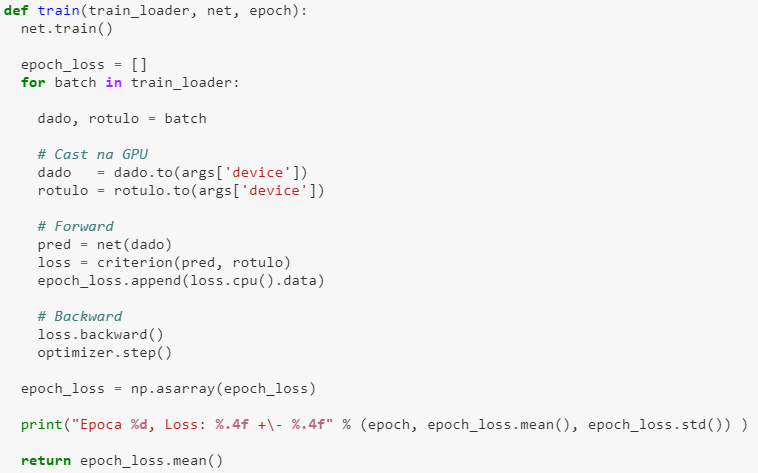
\includegraphics[width=.6\textwidth]{imagens/train.png}}
	
	\label{fig:train}
	{\scriptsize Fonte: compilação do autor}
\end{figure}

\begin{figure}[H]
	\centering
	\caption{Implementação da função de teste da rede}
	\fbox{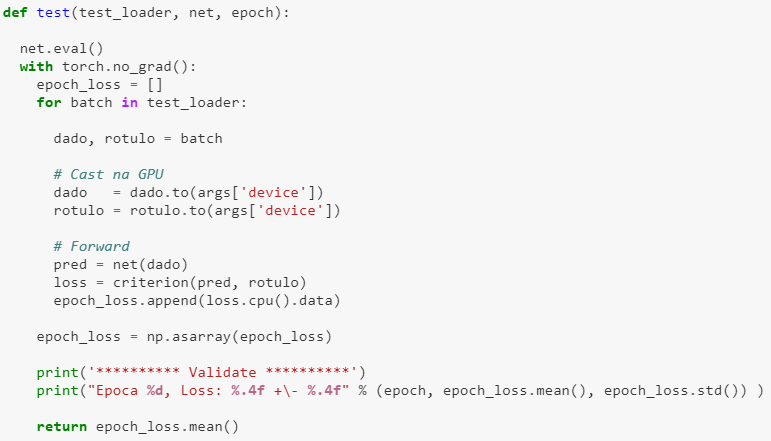
\includegraphics[width=.6\textwidth]{imagens/test.png}}
	
	\label{fig:test}
	{\scriptsize Fonte: compilação do autor}
\end{figure}

\begin{figure}[H]
	\centering
	\caption{Implementação da função que mescla o treino e o teste em uma só}
	\fbox{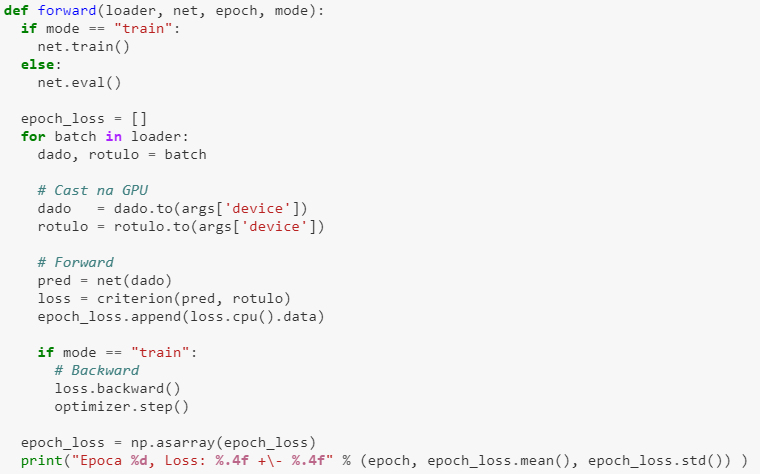
\includegraphics[width=.8\textwidth]{imagens/forward.png}}
	
	\label{fig:forward}
	{\scriptsize Fonte: compilação do autor}
\end{figure}

Como esclarecimento e interpretação visual foi construída, pois, a \autoref{fig:convergencia} com os dados de armazenados de treino e teste (média da \textit{loss function} ou função de custo de cada iteração dentro da época) que mostra um comparativo das épocas de teste e treino da rede neural e a convergência de ambas, retratando a acurácia e a validade do modelo deste experimento.

\begin{figure}
	\centering
	\caption{Convergência das épocas entre o treino e o teste da MLP}
	\fbox{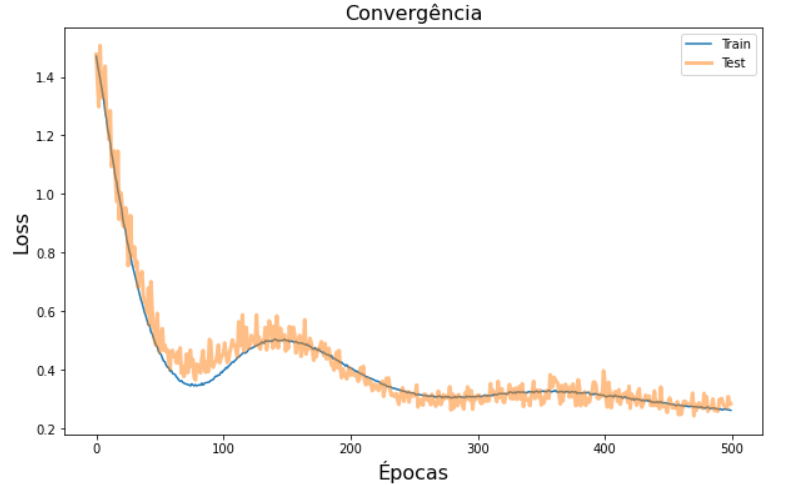
\includegraphics[width=.8\textwidth]{imagens/convergencia.png}}
	
	\label{fig:convergencia}
	{\scriptsize Fonte: compilação do autor}
\end{figure}

A arquitetura da rede neural construída e mostrada na \autoref{fig:mlp-pytorch} pode ser visualizada na \autoref{fig:arquitetura-rede-pytorch} abaixo:

%arquitetura-RNN-vertical
\begin{figure}[H]
	\centering
	\caption{Arquitetura da rede neural}
	\fbox{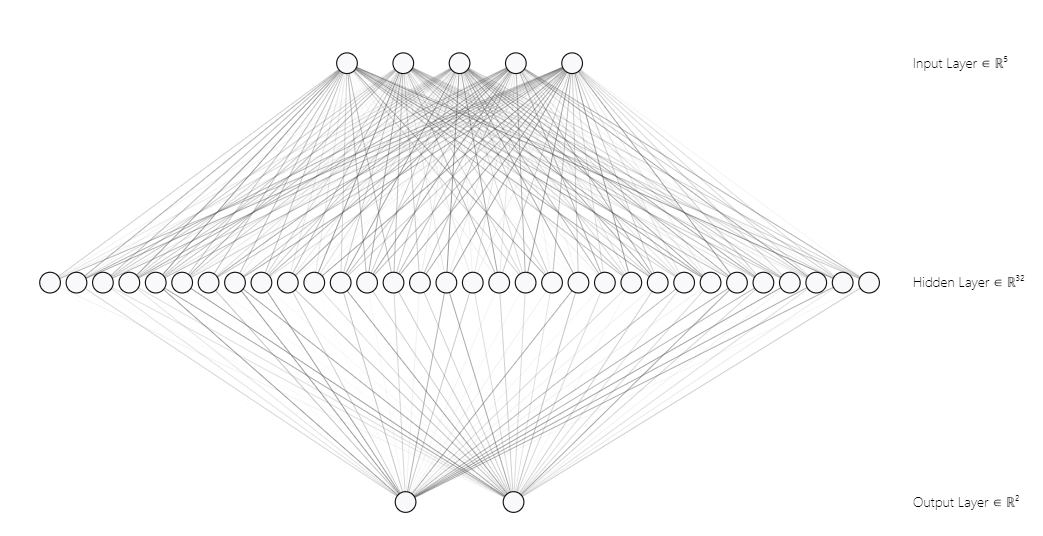
\includegraphics[width=1\textwidth]{imagens/arquitetura-RNN-vertical.png}}
	
	\label{fig:arquitetura-rede-pytorch}
	{\scriptsize Fonte: compilação do autor}
\end{figure}

\section{Teste da detecção de conflitos em tempo de execução}\label{teste}
Para fins de avaliação, foi realizado um teste com um dos modelos dos experimentos (o Random Forest que obteve a maior acurácia) para demonstrar a detecção de conflito em tempo de execução.

Foi gerado um conjunto pequeno de 3 instâncias com o programa \texttt{\textbf{geracao\_politicas.py}} resultando no seguinte \autoref{lst-politicas}:

\begin{lstlisting}[caption={Instâncias geradas aleatoriamente},label=lst-politicas][frame=single][language=Python]
politicas_teste = 
[
  `Obliged',`UFAC',`Secretario_de_Curso_Academico',`Acessar',`Produtos',
  `Permitted',`UFAC',`Secretario_de_Curso_Academico',`Acessar',`Documentos',
  `Obliged',`CCSJA',`Outro_Usuario','Abertura',`Almoxarifado'
]
\end{lstlisting}

Então a lista foi convertida para um DataFrame, tipo de dados do Pandas, no seguinte \autoref{lst-conversao}:
\begin{lstlisting}[caption={Conversão para DataFrame},label=lst-conversao][frame=single][language=Python]
policies_test = pd.DataFrame(np.array(politicas_teste).reshape(3,5), columns = list("ABCDE"))
policies_test.columns = ['Acesso', 'Organizacao', 'Sujeito', 'Acao', 'Objeto']
\end{lstlisting}

O dataframe \texttt{\textbf{policies\_test}} passou pelo processo de encodificação com a função \texttt{\textbf{ManualEncoder.py}} que resultou no dataFrame mostrado na \autoref{fig:policies_test}.

\begin{figure}[H]
	\centering
	\caption{Data Frame com instâncias de teste aleatórias}
	\fbox{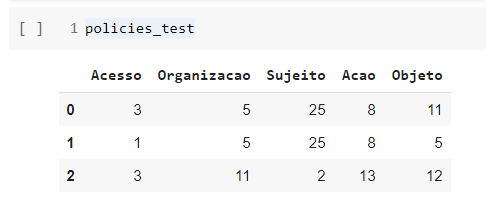
\includegraphics[width=1\textwidth]{imagens/policies_test.png}}
	
	\label{fig:policies_test}
	{\scriptsize Fonte: compilação do autor}
\end{figure}

Foram realizadas as queries (consultas) no dataset mostradas na\autoref{fig:buscas-conflitos}

\begin{figure}[H]
	\centering
	\caption{Data Frame com instâncias de teste aleatórias}
	\fbox{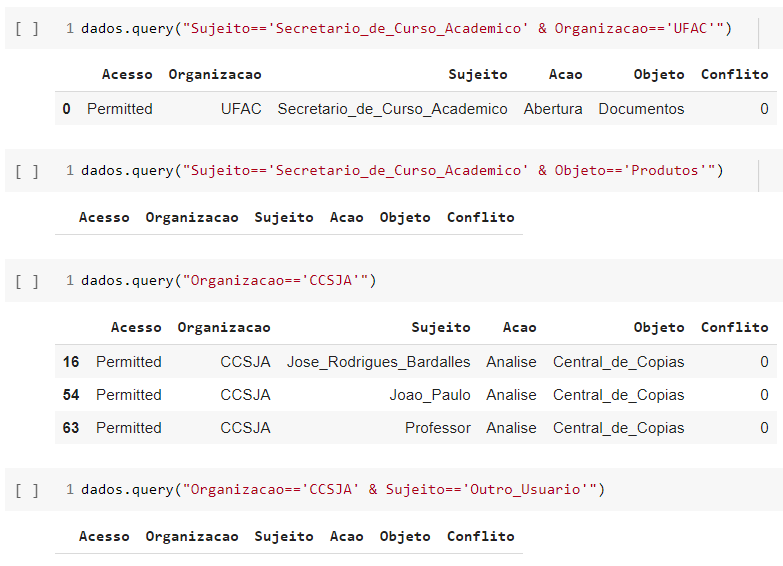
\includegraphics[width=.9\textwidth]{imagens/buscas-conflitos.png}}
	
	\label{fig:buscas-conflitos}
	{\scriptsize Fonte: compilação do autor}
\end{figure} 

Com o \autoref{lst-classifica-certo} criou-se uma lista com as classificações corretas para as instâncias geradas (todas com rótulo `0' significando que não houve conflitos).

\begin{lstlisting}[caption={Listas classificações corretas},label=lst-classifica-certo][frame=single][language=Python]
classificao_teste_correta = [0,0,0] #Sem conflito para nenhuma instancia
\end{lstlisting}

Já com a \autoref{fig:predicao-teste} verificou-se, em tempo de execução e de forma praticamente imediata, baseado no modelo de aprendizagem de máquina criado, que não houve conflito gerando uma nova lista com as predições. A primeira célula do código da imagem mostra os hiperparâmetros do classificador.

%predicao-teste
\begin{figure}[H]
	\centering
	\caption{Resultado da predição em tempo de execução}
	\fbox{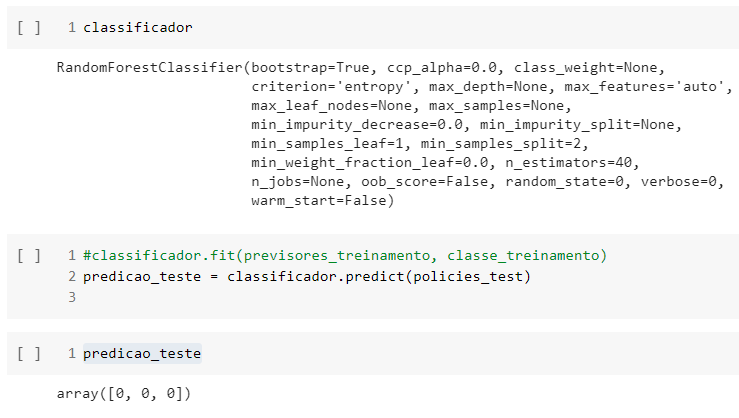
\includegraphics[width=.9\textwidth]{imagens/predicao-teste.png}}
	
	\label{fig:predicao-teste}
	{\scriptsize Fonte: compilação do autor}
\end{figure}

Para finalizar foi criada uma função \texttt{\textbf{compara\_predicoes}} para fazer a comparação das previsões. A \autoref{fig:comparacao-previsao} demonstra isso e a \autoref{fig:resultado-compara} mostra a saída do código.

%comparacao-previsao
\begin{figure}[H]
	\centering
	\caption{Resultado da predição em tempo de execução}
	\fbox{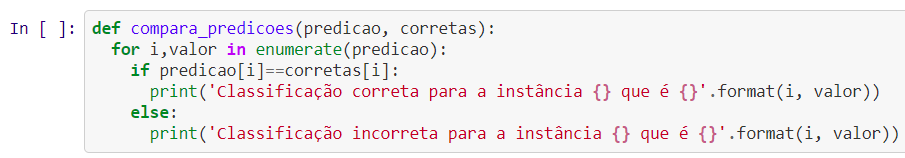
\includegraphics[width=.9\textwidth]{imagens/comparacao-previsao.png}}
	
	\label{fig:comparacao-previsao}
	{\scriptsize Fonte: compilação do autor}
\end{figure}


\begin{figure}[H]
	\centering
	\caption{Resultado da predição em tempo de execução}
	\fbox{\includegraphics[width=.9\textwidth]{imagens/resultado-compara.png}}
	
	\label{fig:resultado-compara}
	{\scriptsize Fonte: compilação do autor}
\end{figure}





\subsection{Análise dos resultados}\label{analise_resultados}
Os experimentos realizados na \autoref{resultados} corroboram a hipótese de que a detecção de conflitos pode ser transformada em um problema da tarefa de classificação da mineração de dados e do aprendizado de máquina. As vantagens sobre as outras abordagens relatadas na literatura são:
\begin{itemize}
	\item A detecção do conflito pode ser realizada em tempo de execução, pois os modelos já estão treinados;	
	\item As políticas são verificadas ``em lote'' e não em pares já que a análise em pares é um problema computacionalmente custoso da classe NP-Completo como demonstrado por \citeonline{shoham_tennenholtz_1995}; 
	\item Ambas as técnicas analisadas neste trabalho mostraram-se eficazes com acurácias acima da proposta inicialmente (95\%) cf. o mostrado na \autoref{exp:139-281}, \autoref{exp:139-281}, \autoref{exp:pandas-numpy-sklearn} e \autoref{exp:tensorflow-pytorch};
	\item os modelos de machine learning desenvolvidos nos experimentos podem ser aplicados em outros contextos, pois são suficientemente genéricos para tal;
	\item Ao analisar uma nova política, não é necessário ``varrer'' ou consultar todas as instâncias do \textit{dataset} novamente já que os modelos já estão treinados;
	\item os modelos de machine learning tem a tendência a melhorarem a eficácia à medida que a quantidade de instâncias cresce
\end{itemize}

Todas os modelos e algoritmos demonstrados nos experimentos tiveram acurácia acima de 95\% o que mostra que a detecção de conflitos em políticas (ou normas) pode ser colocada como uma classe de problemas a serem resolvidos de forma eficiente por técnicas de aprendizagem de máquina.
\clearpage
\chapter{Cronograma e propostas para o texto final}\label{propostas}
Para a pesquisa que resultará na dissertação de mestrado os seguintes pontos serão levantados, estudados e melhor definidos em termos dos objetivos do trabalho:
\begin{enumerate}
\item Finalização da pesquisa teórica sobre funções de custo, SVM, descida do gradiente, suporte matemático aprofundado para o SVM;
\item Revisão Bibliográfica dos classificadores: SVM, Random Forest, Árvore de Decisão e RBF;
\item Finalizar a função de detecção de conflitos indiretos;
\item Comparação final com outros classificadores (preferencialmente, geométricos, como o KNN e o SVM, avaliando suas acurácias e eficiência para os conflitos indiretos.
\item Explorar a detecção dos conflitos indiretos usando Machine Learning e Aprendizagem de Máquina;
\end{enumerate}
Para isso, propõem-se o seguinte cronograma descrito na \autoref{tab:cronograma}
% Please add the following required packages to your document preamble:
% \usepackage{graphicx}
\begin{table}[h!]
	\centering
	\caption{Cronograma de Finalização do Mestrado}
	\label{tab:cronograma}
	\resizebox{\textwidth}{!}{%
		\begin{tabular}{lccl}
			\hline
			\multicolumn{1}{l|}{Atividades Realizadas} & \multicolumn{1}{l|}{jan} & \multicolumn{1}{l|}{fev} & \multicolumn{1}{l|}{mar} \\ \hline
			\begin{tabular}[c]{@{}l@{}}Finalização da pesquisa teórica sobre funções de custo,\\ SVM, descida do gradiente, suporte matemático \\ aprofundado para o SVM\end{tabular} & X &  &  \\
			\begin{tabular}[c]{@{}l@{}}Revisão Bibliográfica dos classificadores: \\ SVM, Random Forest, Árvore de Decisão e RBF\end{tabular} & X & \multicolumn{1}{l}{} &  \\
			Finalizar a função de detecção de conflitos indiretos & X & X &  \\
			\begin{tabular}[c]{@{}l@{}}Comparação final com outros classificadores \\ (preferencialmente, geométricos, como o KNN e o SVM, \\ avaliando suas acurácias e eficiência para os conflitos indiretos)\end{tabular} & X & \multicolumn{1}{l}{} &  \\
			\begin{tabular}[c]{@{}l@{}}Explorar a detecção dos conflitos indiretos usando \\ Machine Learning e Aprendizagem de Máquina\end{tabular} & X & X &  \\
			Escrita, revisão e entrega da versão preliminar & \multicolumn{1}{l}{} & X &  \\
			Conclusão do artigo para envio para periódico & \multicolumn{1}{l}{} & X & \multicolumn{1}{c}{X} \\
			Entrega do Texto final e defesa & \multicolumn{1}{l}{} & \multicolumn{1}{l}{} & \multicolumn{1}{c}{X} \\ \hline
		\end{tabular}%
	}
\\[6pt]	\centering {\footnotesize Fonte: Elaborada pelo autor}
\end{table}

\chapter{Conclusões}\label{conclusoes}
\begin{itemize}
	\item Esta pesquisa mostrou a possibilidade de \textit{converter a detecção de conflitos a um problema de classificação} especificamente, para os conflitos \textbf{\textit{diretos}};
	\item O classificador mais acurado, nos experimentos, foi, como se imaginava pela hipótese, o \textit{MultiLayer Perceptron} que é um classificador que usa \textit{backpropagation} para aprender usando perceptron de várias camadas para classificar instâncias desconhecidas \cite{eibe2016};
	\item Será realizada uma comparação entre o MLP e o SVM (e outros classificadores geométricos). Suas acurácias serão devidamente comparadas juntamente com a eficiência das soluções propostas.
	\item Todas os modelos e algoritmos demonstrados nos experimentos tiveram acurácia acima de 95\% o que mostra, portanto, que a detecção de conflitos em políticas pode ser colocada como uma classe de problemas a serem resolvidos de forma eficiente por técnicas de aprendizagem de máquina.
\end{itemize}